\documentclass[letter,12pt]{article}
\usepackage[letterpaper,right=1in,left=1in,top=1in,bottom=1in]{geometry}
\usepackage{setspace}

\usepackage[utf8]{inputenc}   % allows input of special characters from keyboard (input encoding)
\usepackage[T1]{fontenc}      % what fonts to use when printing characters       (output encoding)
\usepackage{amsmath}          % facilitates writing math formulas and improves the typographical quality of their output
\usepackage[hyphens]{url}     % adds line breaks to long urls
\usepackage[pdftex]{graphicx} % enhanced support for graphics
\usepackage{tikz}             % Easier syntax to draw pgf files (invokes pgf automatically)
\usetikzlibrary{arrows}

\usepackage{mathptmx}           % set font type to Times
\usepackage[scaled=.90]{helvet} % set font type to Times (Helvetica for some special characters)
\usepackage{courier}            % set font type to Times (Courier for other special characters)

\usepackage[longnamesfirst, sort]{natbib}\bibpunct[]{(}{)}{,}{a}{}{;} % handles biblio and references 

\usepackage{rotating}         % sideway tables and figures that take a full page
\usepackage{caption}          % allows multipage figures and tables with same caption (\ContinuedFloat)

\usepackage{dcolumn}          % needed for apsrtable and stargazer tables from R to compile
\usepackage{arydshln}         % dashed lines in tables (hdashline, cdashline{3-4}, 
                              %see http://tex.stackexchange.com/questions/20140/can-a-table-include-a-horizontal-dashed-line)
                              % must be loaded AFTER dcolumn, 
                              %see http://tex.stackexchange.com/questions/12672/which-tabular-packages-do-which-tasks-and-which-packages-conflict


\newcommand{\mc}{\multicolumn}

%% TO ADD NOTES IN TEXT, PUT % BEFORE THE ONE YOU WANT DISABLED
%\usepackage[disable]{todonotes}                            % no show
\usepackage[colorinlistoftodos, textsize=small]{todonotes} % show notes
\newcommand{\emm}[1]{\todo[color=red!15, inline]{\textbf{Eric:} #1}}
\newcommand{\vp}[1]{\todo[color=green!15, inline]{\textbf{Vale:} #1}}
\newcommand{\ges}[1]{\todo[color=blue!15, inline]{\textbf{Ges:} #1}}

\usepackage{xr} % allows cross-ref to other file
\externaldocument{urge14appendix}

% agradecimientos
% Sebastián Soto Velasco, ex-director jurídico de del ministerio secretaría general de la presidencia
% Roberto Bustos, Secretario de la Comisión de Hacienda del Senado
% Alvaro Villarroel, staff Comisión de Hacienda del Senado
% Tercer staff de Comisión de Hacienda del Senado
% Dip. Patricio Vallespín
% Dip. 1er vice-presidente de la Cámara de Diputados

% [28-8-2017] improvements for logit
% a. drop member bills or analyze separately
% b  control whether or not bill was reported: this is gatekeeping
% b.1  analyze this as a separate DV
% b.2  use a conditional model: not reported are not same type
%    |    | U   | ~U  |
%    |----+-----+-----|
%    | G  | g_u | g_s |
%    | ~G | u   | s   |
%    |----+-----+-----|
 

\begin{document}

  

\title{Presidents on the Fast Track: Fighting Floor Amendments with Restrictive Rules\thanks{The authors are grateful to Roberto Bustos, Alvaro Villarroel, and the staff of the Chilean Senate's Hacienda Committee, and especially to Sebastián Soto Velasco for help understanding urgency authority; to Diputado Patricio Vallespín for making the calls that scheduled interviews with key congressional personnel; to Mónica Arretche, Ernesto Calvo, José Antonio Cheibub, Federico Estévez, Adrián Lucardi, Michelle Taylor-Robinson, and participants at the 2017 annual meeting of the American Political Science Association in San Francisco, at the Evolution of Parliamentarism Workshop in Rome, and at the IV encuentro del Grupo de Estudios Legislativos de ALACIP in Mexico City for comments and critiques. Eric Magar acknowledges financial support from the Asociación Mexicana de Cultura A.C.\ and CONACYT's Sistema Nacional de Investigadores. Valeria Palanza acknowledges support from Proyecto Fondecyt No.\ 1140974. Gisela Sin acknowledges the support of the Office of the Vice Chancellor for Research and the Center for Latin American Studies, University of Illinois at Urbana-Champaign. The authors are responsible for mistakes and shortcomings in the study.}}
\author{Eric Magar \\ ITAM \and
        Valeria Palanza \\ Univ.\ Católica de Chile \and  
        Gisela Sin \\ University of Illinois
}
\date{\today}
\maketitle

%\begin{center} \textbf{$\rightarrow$~~Preliminary draft~~$\leftarrow$} \\ (please inquire for new version, \small{\url{emagar@itam.mx}})  \end{center}

\begin{abstract}
\noindent Among presidents' lesser known legislative powers is urgency authority. Seven Latin American presidents wield it: the constitutional power to impose on lawmakers a short deadline to discuss and vote selected bills. This power is similar to the fast-track authority that Congress grants periodically to the U.S.\ president. We claim that the key consequence of urgency authority is procedural: urgency prevents amendments during floor consideration. By using fast track authority, presidents can protect bills and committee agreements; in essence becoming a single-member Rules Committee with ability to impose closed rules on the floor. A formal model generates hypotheses that we test with original data from Chile between 1998 and 2014. Results confirm that preference overlap between the president and committee chairs drives the use of fast track authority systematically. Patterns in Chile are reminiscent of restrictive rule usage in the U.S.
\end{abstract}

% comentarios de Calvo
%Comentarios a Magar: Presidential obstruction of the agenda in Chile’s Congress
%Buenísimo el paper. Siempre me pareció muy interesante el tema de las urgencias y no existen análisis sistemáticos de estos procesos. Tengo muchas ganas de ver el libro completo una vez que esté terminado. 
%En términos generales me gusta mucho la perspectiva y el modelo es interesante. El juego está descripto con poco detalle (supongo que eso viene en otros capítulos) así que la presentación de la Figura 2 y su discusión en las páginas 10 y 11 siguen siendo un poco crípticos. La intuición se entiende, pero el hecho de que en distintos sistemas k y o toman distintos valores y producen distintos equilibrios necesita más fundamentación (de nuevo, asumo que eso viene de capítulos anteriores del libro). 
%El capítulo preguntando porque los legisladores toman en consideración las ``urgencias'' cuando a diferencia de Brasil o Uruguay no existe un mecanismo de sanción si ellos ``shirk''. No tenemos respuesta a lo largo del capítulo y mi impresión es que se necesita un poco mas de data cualitativa (algunas entrevistas o discusiones de diarios de sesiones) que digan porque los legisladores atienden al pedido del presidente. Esto quizá afecte como pensas el modelo de la Figura 2 y te convendría resolverlo antes de cerrar el capítulo.
%Mi preocupación principal está en la forma en que usas la data y como estimas el modelo. Las ``urgencias'' son un mecanismo para presionar al Congreso para que actúe y, por tanto, tienen que ser modelados con una función de tiempo. Lo más natural para mí sería utilizar un ``mixture'' model que mide al mismo tiempo la ``tasa'' de aprobación y el ``tiempo'' de aprobación (te anexo un artículo en el cual hacemos esto para el caso de Uruguay con Chasquetti). Entiendo que las ``urgencias'' son una forma de presionar al Congreso para resolver favorablemente, pero la discusión sobre el ``scheduling'' del plenario también refiere al problema del costo de oportunidad de tratar los proyectos del Presidente en lugar de los proyectos de los legisladores. Sin embargo, todos los Congresos tienen mecanismos para permitir que los ``pet projects'' sean aprobados cuando hay tiempos limitados en el plenario. En Brasil las comisiones pueden dar aprobación final a una gran cantidad de projectos (``terminativa'') para evitar consumir el tiempo del plenario. En Argentina el artículo 133 del reglamento permite votar en paquete proyectos que tienen dictamen de comisión y no tienen objeciones ni enmiendas. Por lo tanto, existen cambios en las reglas que les permiten a los legisladores ``circunvent'' las restricciones de tiempo del plenario. Para mi es necesario modelar el éxito relativo y el tiempo de aprobación para ver que es lo que están haciendo las urgencias.
%Esto también quiere decir que el modelo de estimación debería ser al nivel de proyecto de ley y no un OLS con sumas de instancias. Sino me equivoco tenes toda esa data, el N es mas grande y además te permite combinar data a nivel de proyecto, de legislador y de Congreso. Así que a mi juicio conviene cambiar la estrategia de estimación. 
%Por lo demás, me parece un excelente artículo y me muero de ganas de ver el libro.
%Abrazo. E.  

% Adriana Alfaro
% En Chile se llama urgencia, en Mx iniciativa preferente. Cómo se llama en Colombia etc? La lectura semántica quizás sesgó la interpretación de Morgenstern y cia.

% R: No parece ser el caso, sólo en México no lleva el mote de 'urgente'.
%    Colombia = manifestación de urgencia
%    México   = iniciativa preferente
%    Brasil   = urgencia para apreciación
%    Uruguay  = declaratoria de urgente consideración

% Adrián:
%
%% Hola Eric,
%
%% Muy bueno el paper. Me parece que la colaboración presidente-comités es muy interesante, y además de ver qué proyectos son declarados urgentes, el modelo probablemente tiene otras implicaciones que pueden desarrollar después.
%
%% Como te dije, acá te mando un par de comentarios adicionales:
%
%% 1. No estoy seguro si el comienzo de la sección 2 (pp. 4-6) es el mejor lugar para discutir la data y los tipos de proyectos de urgencia. Tal vez sería mejor comenzar con el ejemplo y el modelo (más algunos ejemplos de la vida real) y recién al ir al caso de Chile discutir los datos y los distintos tipos de urgencia.
% R: done.
%
%% 2. Una cosa que no me quedó 100% clara, y se podría aclarar: ¿lo de los distintos tipos de proyectos de urgencia está en la Constitución, o en los estatutos del Congreso?
%  R: lo decimos en el texto y elaboramos en una nota a pie.
%
%% 3. En la presentación mencionaste distintos tipos de quórum para distintos tipos de proyectos. En la medida en que sea fácil determinar qué tipo de quórum amerita cada proyecto, se podría partir la muestra para ver si los resultados son similares cuando se requiere quórum simple o una mayoría especial, etc.
%
%% 4. Casi todas las variables son dummies entre 0 y 1. La variable Year remaining varía entre 0 y 100, ¿por qué no dividirla por 100 para que quede en la misma escala que el resto?
%
%% Por último, algunas posibles extensiones que tal vez sea mejor discutir en otros trabajos, pero podrían mencionar en la conclusión:
%
%% 5. No me quedó clara la diferencia entre poder de urgencia y poderes de decreto, especialmente cuando hay aprobación automática (e.g., Uruguay). Pero si el presidente puede legislar por decreto, ¿el pleno no tiene que elegir entre el decreto tal como está, o introducirle algo? O sea, ¿el decreto no funciona también como una closed rule? No lo digo por el caso chileno, pero sí para pensar cómo comparar con otros países.
%R (gisela); el decreto es mas fuerte que todo lo que conocemos.  Hasta el fast-track authority the Howell y Moe tiene que ser aprobado por el Congreso, pero en Argentina por ejmeplo, los decretos no estan reglamentados y no necesitan ser aprobados por el congreso. (VP: ojo esto ya no es más así, ahora los decretos requieren aprobación del congreso, ya se creó la comisón mixta) Otra cosa: la gran diferencia seria si los decretos se analizan en comision o no.  En Chile, la comision puede introducir todos los cambios que quiere (y creo que es asi en Brazil, no?) . No se si es asi en Argentina. Este closed rule en Chile defiende el bill de amendments no negociadas con el presidente de la comision (que pueden venir de facciones del partido/coalicion gobernante, o de la oposicion).
%
%% 6. ¿El modelo genera algún otro tipo de predicciones? Ustedes están mirando declaración de urgencia, ¿pero es posible predecir qué proyectos deberían morir en el comité, cuáles deberían ser aprobados por el pleno, cuáles recibir enmiendas, etc? Si no es posible predecirlo (o no tienen los datos para evaluar las predicciones), deberían explicar por qué en el paper. Se me hace que muchos reviewers les van a salir con eso.
%Valeria: sí, el modelo permite predicciones de este tipo, de hecho hacemos predicciónes de cuándo no se impondrá urgencia, y los escenarios que se abren en ese caso... No evaluamos eso porque es para otro paper, pero habría que mencionarlo.
%
% falta un resumen del paper, predicciones, estrategia empirica etc en intro; mencionar que es más instrumento de colaboración que acelerador. Qué hace el paper?
% No Moe&Howell, sólo que es análogo al fast-track de tratados internacionales


% Otros comentarios de la charla en el itam
% 1. Jeff: In US, committee reports original bill and amendments separately, each voted. 	NOT TRUE: REPORTS A BILL DEPENDING ON HOW WAS THE FINAL OUTCOME WITH THE VOTES ON THE AMENDMENTS. IN THE RPORT OF COURSE IT MAKES A SUMMARY OF THE DENATE, THE AMENDMENTS, THE VOTING, WHO OTED FOR WHAT, ETC.  VERY SIMILAR TO CHILE. In Mexico, committee reports its own version. Is it the same in Chile? EMM: Yes, methinks. FEE: Look at original executive proposals and what the committee reports, to see how much change there was. GS: HAHA THAT'S A LOT, LOT OF WORK 
%
% 2. FEE/Adrián: analize exv bills urgent since the beginning vs those declared urgent later. Should hint at how restrictive rules become necessary as exv makes concessions in original bill... 
% GS: WHAT DO YOU THINK ABOUT THIS? NOT SURE HOW IT WOULD MATTER, BUT NOT IN THAT WAY. THE RESTRICTION DOE SNOT COUNT FOR COMMITTEES. BUT THE DIFFERENCE SHOULD BE INTERESTING: WHY SOME HAVE URGENCY SINCE THE BEGGINNING? I IMAGINE IT HAS TO DO WITH A SIGNAL FROM THE EXECUTIVE: THE BILL IS IMPORTANT, AND I AM WILLING TO SHIELDED FORM AMENDMENTS IN THE FLOOR IF YOUDO NOT MODIFY IT MUCH. OR MAYBE SOMETHING LIKE: THIS IS IMPORTANT TO ME, I'M WILLING TO NEGOTIATE
%
% 3. Vidal: discuss why the institution is so much used and has survived so long. Also: why aren't all exv bills urgent? (R: if comm introduced changes, P may want floor to ``correct'' them. 
%
% 4. FEE: Senate, where opp sometimes controlled, seem more attractive test. 
%
% 5. Micozzi: controlar sesiones extraodinarias, en particular en dic-marzo.
%
% 6. Adrián: recode para que en caso de multiple referral, coalChair=1 sólo si todos son de coalición.
%
% 7. Multiple referrals: simultáneos o secuenciales? Cómo opera el gatekeeping?
% GS: ACCORDING TO SOTO, SE PUEDEN MANDAR PROYECTOS A UNA O MAS COMISIONES, QUE PUEDEN ACTUAR SEPARADAS O UNIDAS. , O TAMBIEN PUEDE ENCONMENDARSE A UNA COMISION ESPECIAL.  (TODO ESTO ES DEICISION DEL PRESIDENTE DE LA CAMARA)  SI SON SEPARADAS,  PUEDE HABER UNA COMISION PRIMARIA, QUE SI APRUEBA EL PROYECTO ENTONCES SE TRATA EN EL PLENARIO. SI LA COMISION SECUNDARIA NO APRUEBA ELPROYECTO, IGUAL PUEDE IR AL PLENO.  PERO TAMBIEN SE PUEDE ENVIAR UN PROYECTO A COMISIONES UNIDAS: ESTO ES, LAS COMISIONES TIENEN QUE REUNIRSE JUNTAS Y TRATAR EL PROYECTO DE LEY . CON ESTO ULTIMO BASICAMENTE SE MATA EL PROYECTO.
% 
% 8. Simpser: policy area descriptives, need to show that result is not this rather than committee chair. Check speed controllingthis, too.
%
% 9. FEE: cotejar la propuesta original vs el reporte primero, para evaluar la discreción del committee chair. También, contar historia de uno o dos bills como ejemplo de perro que ladra/no. 
%
% 10. FEE. Controlar margen de victoria en el pleno.

%% DE VALERIA

%% (b) pedirle a un RA que haga una investigación rápida (creo recordar que el reglamento no es muy explícito) para entender la práctica de introducción de indicaciones, en general,

%% No conseguí RA porque es época de exámenes, pero esto es lo que pude ver yo. Hay 55 referencias a indicaciones en el reglamento, así que esto intenta resumir lo más importante:
%% - El reglamento de 2015 (el único sobre el cual hay claridad al momento) establece que el Presidente de la cámara puede declarar inadmisible las indicaciones (art 55.2).
%% - Aparte, los proyectos que formen parte de la tabla de Despacho Inmediato no podrán ser objeto de indicaciones y serán sometidos a una sola votación.
%% - En los proyectos incluidos en la tabla de Fácil Despacho las indicaciones presentadas serán tratadas una vez aprobado el proyecto en general, pero no se aceptarán indicaciones en materias de la Comisión de Hacienda, esas indicaciones serán enviadas a la Comisión de Hacienda. Las indicaciones se pueden presentar hasta el momento antes de que se vote el último artículo que se trate en particular.
%% - Si no hay indicaciones, la aprobación en general incluye la aprobación en particular del proyecto.
%% - Durante la discusión general el Presidente de la República y los diputados pueden introducir indicaciones.
%% - Bastará que un comité solicite plazo para formular indicaciones para que sea otorgado, no pudiendo el plazo ser inferior a un día.
%% - Se someterán a discusión en particular las indicaciones que, rechazadas en el segundo informe, sean renovadas por el Pdte de la República o por dos jefes de comités.
%% - Se llama también "indicaciones" a las mociones para reabrir el debate y otras mociones.
%% - No se admiten indicaciones que alteren gastos por parte de diputados. Sólo se admitirán si emanan del Pdte de la Rep.
%% - Sí si disminuyen gastos.
%% - Cuando se trate de proyectos con suma urgencia o discusión inmediata sólo serán aceptadas indicaciones rechazadas por las comisiones informantes si son respaldadas por la firma de 30 diputados que incluyan al menos a 3 jefes de comités, siempre que se trate de las que fueron presentadas en la discusión en general o dentroo del plazo fijado por la cámara.
%% - El pdte de la cámara es quien puede declarar inadmisibles indicaciones.

%% y si alguien además del presidente puede imponer closed rule---ie, prescindir de la segunda lectura---en particular. 

%% Todos los proyectos incluidos en la tabla de Fácil Despacho no tienen segundo informe de comisión. Son proyectos de poca importancia. Todos los órdenes del día tienen tabla de fácil despacho. Pero la mesa que decide qué entra en esta tabla tendría esa prerrogativa, y podría "estirar" su uso. 

%% Creo mencionar un una nota a pie un recurso de la biblioteca del congreso que resume bien la práctica parlamentaria. 

%% No consulté esto, mi única fuente fue el Reglamento 2015. 

%% 2. Sigue también pendiente encontrar una versión del reglamento de la cámara anterior a 2010 para verificar si la closed rule antes aplicaba sólo a la suma urgencia.

%% Adjunto memo sobre reglamento 2015 que tiene, al principio, todas las enmiendas al reglamento. Después, un resumen de todo lo que se dice en el Reglamento acerca de las urgencias. Las reformas, para hacer lo mismo hacia atrás, son muchas, habría que ver cuáles nos interesan. Eric, si tienes en mente una en particular, dime cuál. Le encargaré a un RA hacer el seguimiento de los artículos que yo identifiqué en el Regla 2015 hacia atrás, pero es un trabajo tremendo así que si lo podemos acotar, mejor.

%% 3. Algunas ideas para un nuevo título que aluda a Relic:

%% -Presidential fast-track authority: More a Previous Question than a privileged motion
%% -Not faster/Not an accelerator but a shield against plenary amendments
%% -Not a car pool lane but a cloture of highway exits
%% -Presidents with fast-track authority who cannot accelerate
%% -Not an accelerator, a take-it-or-leave-it rule

\newpage

\doublespacing

\section{Introduction}

\noindent It is well established that presidents have a variety of prerogatives to achieve their legislative goals. Most common and best known is the veto, a president's final say on new legislation. Scholarly attention has recently turned towards executive decree powers, a centerpiece in many Latin American constitutions. Considered initially a tool to encroach upon the legislature's powers, we know now that constitutions vary in the extent to which they involve assemblies in the approval of decrees. Our interest is in the urgency authority, a much less known tool that enables presidents to actively participate in the lawmaking process. Urgency authority gives executives power to set the legislative agenda by imposing a requirement to hold a vote within a short period of time. With this, presidents earn the ability to interfere with Congress' voting schedule and floor control. This, in itself, is worth analysis.

Urgency authority seems to contradict classic notions of separation of powers. The Framers of the United States Constitution warned against expediting lawmaking and arresting deliberation---``In the legislature promptitude of decision is oftener an evil than a benefit'' \citep{hamilton70.1788}. They saw the ability to put a final negative as a sufficient presidential check on legislation. Despite warnings and concerns, seven presidential systems of the Americas give their executives urgency authority of some form: Brazil, Chile, Colombia, Ecuador, Mexico, Paraguay, and Uruguay \citep{morgenstern.nacif.2002,garcia.montero.presidentes.2009}.
%``The magistrate in whom the whole executive power resides cannot of himself make a law, though he can put a negative on every law'' argues \citet{madison.47} in Federalist 47. 

We examine constitutions across the Americas and describe institutional similarities and differences in urgency authority. Most striking is that in some cases urgency power is not binding, as is the case in Chile. That is, no formal consequences follow legislators' non-compliance with deadlines: failure to act speedily neither stops the whole legislative process nor automatically turns the bill into law, as occurs elsewhere. On average, three of every five bills that Chilean presidents sponsor become urgent at some stage of the legislative process. If there are no consequences for non-compliance, why would presidents routinely rely on a power that is inconsequential?
%Chile is of special interest because it is the sole case where urgency authority has received more or less systematic attention.

This puzzle led us to inspect legislative standing rules for clues. We did not find the missing penalty there either, but discovered an interesting twist in this institution: urgent legislation is considered under a closed rule. Closed rules are one form of restrictive procedure: when a bill reaches the floor under such a rule, legislators cannot offer any amendments \citep{oleszek.2001}. They simply vote the bill up or down. This is exactly what happens in the U.S. with legislation that reaches Congress under the fast-track authority the president has to negotiate international trade.
%Chilean sub-constitutional institutions therefore equate urgency power to the fast-track authority granted periodically to the United States President by Congress to negotiate international trade.

We claim that urgency authority of the fast-track type increases significantly the executive's influence on lawmaking because it gives presidents the ability to decide whether to impose restrictive procedures or leave bills open for amendments on the floor---and not, as intuition might suggest, by speeding up the consideration of bills. We model urgency authority formally in order to show this. Our argument joins a growing literature on restrictive rules in legislatures worldwide.\footnote{E.g., \citet{dion.huber.1996,doring.restrictiveRules.2003,huber.1996b,krehbielRestrictiveRules1997,heller.2001,weingast.1992,schickler.richRules1997,cox.mccubbins.1997,amorim.cox.mccubbins.2003,calvo.2014argBook,sin.2014,denhartog.2004phd}.} Closed rules in general, and fast-track authority in particular, protect the agreements reached in committee from being undone later on the floor. What makes urgency authority worth investigating is that the president joins legislative leaders in deciding whether a bill proceeds to the floor with a closed rule or is open for floor amendments.

However, what is the true added-value of urgency authority when presidents can also issue decrees to adopt policy with no intervention from the legislature? Ten Latin American constitutions endow their presidents with this unilateral power, three of which (Brazil, Colombia, and Ecuador) include urgency authority too. If the goals of urgency authority---i.e., to speed up the legislative process and to warrant laws close to the president's preferences---can also be achieved through decrees, why would presidents resort to urgency authority? We argue that presidents that may issue decrees often rely on the statutory path instead, and for reasons that are not precisely associated to lack of haste---e.g., to render policy more robust to challenges in courts or bring confidence to financial markets \citep[cf.][]{palanza.2019}. In those cases, urgency authority becomes a valuable tool giving presidents increased leverage over the statutory path.  

We test our model with original data taken from Chilean bill histories. A systematic analysis of all bills in the 1998--2014 period provides evidence supporting the key implications of our theoretical model. First, that the closer the preferences between the president and the chair of the reporting committee, the higher the probability the president will use his fast-track authority to shield a bill from floor amendments. Second, that when the committee chair with jurisdiction over a bill belongs to the opposition, the probability the bill will be debated on the floor under an open rule increases. By making amendments possible, the open rule lets the floor bring the bill back to the floor (or party) median, as way to discipline unruly commmitee chairs.

The paper proceeds as follows. Section 2 describes urgency authority in Latin American constitutions while engaging with the literature. In section 3 we delve into fast-track authority in the United States, emphasizing how it can be used not only to speed up the legislative process, but also to protect bills from floor amendments. We show how the sequence of committee reports and floor readings makes it harder to introduce floor amendments to urgent than non-urgent bills. Section 4 extends a simple model of restrictive rules from the U.S.\ House of Representatives to fast-track authority. The spatial model highlights the logic behind the procedural choice: when the executive anticipates that a committee report of her liking is vulnerable to floor amendments, she imposes a take-it-or-leave-it vote on the floor by declaring it urgent. When the executive anticipates a commite report far from her preferences, she allows it to come to the floor under an open rule, so that friendly legislators will be able to introduce amendments. We derive testable hypotheses. Section 4 offers a test with data from Chile. The analysis reveals that bills reported by committees chaired by the president's party/coalition have a higher probability to become urgent. Section 5 elaborates implications of our model and findings for the study of separation of powers systems. 
% other features constant

%Every Latin American constitution granting urgency authority remains silent about the closed rule, explaining why comparative politics has overlooked the key feature of this institution. But, in the Chilean case at least, inspection of the chamber's standing orders reveals that presidential urgency qualifications entail precisely such a restrictive procedure in the floor consideration of a bill.

\section{Constitutional Urgency Authority}

Urgency authority confers agenda setting power to the president. This takes place on two fronts. First, the ability to bring bills to the fore for floor consideration allows the executive to prioritize legislative business. When a bill is denoted urgent, it takes the next place in line, and other bills get pushed back. Second, by setting a deadline, presidents can force legislators to decide on thorny issues that many legislators would have otherwise preferred to keep dormant.\footnote{Note that although presidential threats to hijack floor time might suffice to obtain concessions in bargaining, we do not take this line of argument here. Instead, we focus on how the ability to manipulate procedures confers presidents political influence.} 

The cross-national study of urgency authority is scant and mostly descriptive. The influential volume on Latin American legislatures by \citet{morgenstern.nacif.2002} mentions urgency authority's relevance without further examination. \citet{garcia.montero.presidentes.2009} intersects this authority with other institutional features in a typology of Latin American presidents. She argues that the greater presidential power to force debate and vote proposals, the greater the presidential influence in the legislative process, and identifies seven constitutions in the region that include urgency prerogatives. \citeauthor{aleman-tsebelis-2016-book}' \citeyearpar{aleman-tsebelis-2016-book} edited volume on lawmaking in Latin America lists urgency authority among the president's agenda-setting tools. Their analysis is valuable by situating this power in contrast with other tools. In the concluding chapter, the authors explain that presidents ``use urgency motions to prioritize bills in the congressional calendar'' (229). 

Urgency authority varies across constitutions. We distinguish three types, depending on the consequences of legislative non-compliance with the urgency requirements: floor arrest, automatic adoption, and indeterminacy. Brazil has the first type: the president can declare ``urgent'' an executive-sponsored bill at any point in the legislative process, and each chamber of Congress has forty-five days to consider and vote it. If the chamber fails to do so, floor activity comes to a halt until it approves or rejects the urgent bill. While \citet{hiroi-renno-2016} find that urgent bills have better odds of passing, \citet{figueiredo.limongi.2000} report that the prerogative is seldom used as presidents prefer to rely on the more versatile power to issue decrees. While these results are not at odds with our argument, they aim at understanding different aspects of urgency power: its effect on legislative success and the determinants of levels of reliance. Our aim in this paper is to uncover the mechanisms that may make the urgency prerogative a more enticing power than we had previously noticed. We return to this point later in the article. %If this preference is not at odds with our argument---to make the urgency prerogative a more enticing power than we had previously noticed by showing its hidden effect on lawmaking and determinants of levels of presidential reliance---we return the urgency/decree interaction later in the article, as it deserves closer attention.

The constitutions of Ecuador, Paraguay, and Uruguay have the automatic adoption variant. If Congress fails to act within a pre-specified, short period on bills qualified as urgent, they become law. Urgency authority of this type, akin to France's \emph{vote bloqué} \citep{huber.1996b}, increases the legislative influence of the president significantly. And by allowing presidents to replace the status quo with a law without any congressional action, it also resembles decree power \citep{carey.shugart.1998}. These three constitutions, however, also set limits on the presidential prerrogative. The Uruguayan does so by giving Congress one-hundred days to consider urgent legislation, and is the most restrictive. A single bill can be qualified as urgent at any given time, and budgets as well as bills requiring super-majorities for passage are excluded. More significantly, three-fifths of either chamber's membership can override the urgency. \citet{chasquetti.2016} reports that since 1967, when it was adopted, only fourteen bills have received urgent qualification, of which eight became law. He also acknowledges that the main motivation for using it was to force standing committees to discharge bills that they were holding up. The 1998 and 2008 Ecuadorean constitutions give the assembly thirty days to modify, approve or reject urgent bills, and also constrain the president by limiting the number of bills that she can qualify as urgent to only one bill at a time, and only bills on economic issues \citep{morgenstern-polga-shair.2013}. Finally, the Paraguayan constitution, granting Congress thirty days to consider and vote urgent legislation, is the most permissive: the president has latitude to declare bills of any type urgent, at any point during the legislative process.

The cases of Chile, Colombia, and Mexico are indeterminate. While all mandate a thirty-day period for each chamber to consider and vote bills that presidents qualify as urgent, and place minimal restrictions to the type of legislation eligible (the Mexican case limits it to two bills every semester, and the Chilean case allows all bills except budgets to be declared urgent), none sets a reversionary outcome---i.e., plenary arrest or automatic adoption---if the legislature does not act by the deadline \citep{nolte.2003,sotoCongChile2015,carroll-pachon.2016,magar.2014-refConst}.

We are unaware of studies of urgent bills in Colombia and Mexico. But Chile's urgency authority has been examined rigorously, uncovering the paradox in the introduction. Very few acceleration effects are discernible. \citeauthor{siavelis.2002}' \citeyearpar{siavelis.2002} study of Chile's first post-transition administration shows a mild improvement in the pace of executive-initiated bills declared urgent, which take about 19 weeks until they reach the floor, compared to the rest, which take almost 23 weeks. Meanwhile, the effect on passage is nil: The success rate of executive bills was 64 percent when urgent, 63 when not. The set of bills receiving urgent status is not random and that is an obstacle to measure effects properly. On top of this, \citet[][:51]{nolte.2003} argues that urgent bills still need congressional support to become law, so the size and discipline of the president's congressional majority remains the determinant factor for success, not urgency authority. 

Given that in Chile urgency authority does not seem to expedite legislation much nor make passage any likelier, common sense suggests that presidents should rarely use it. But this is not the case: about 60 percent of executive proposals are declared urgent at some point in the legislative process. To confront this paradox, others note that, despite the lack of teeth, Chilean urgency authority may operate as a signalling device \citep{berrios.gamboa.fiscChile.2006,aninat.exagCoop2006}. \citet{aleman.navia.UrgChi.2009} argue that bills that qualify as urgent encompass the president's legislative priorities. Distinguishing degrees of urgency (see footnote \ref{fn:supreme}) they find that ``bills that receive [the top degrees of] urgency motions appear significantly more likely to pass'' (404) than the rest. Although this finding shows that the president's priorities do become law, it is unclear what mechanism is behind the urgency qualification.

\section{Fast-track authority and the closed rule}

The case of the United States offers another clue. The U.S.\ is different from Latin America in three respects. It grants presidents fast-track authority on a single issue, international trade. It does so through statutes with a sunset clause, not the constitution. And, most importantly for our argument, it explicitly constrains legislative choices during floor consideration of bills on the fast-track. We elaborate each in turn.

The first difference resonates with cases such as Ecuador or Uruguay, by further restricting the scope of urgency authority. Trade Promotion Authority, as urgency is formally called in the U.S., is applicable to international trade agrements only. NAFTA is perhaps the most notable achievement, but agreements with a dozen other partners have gone into effect through fast-track in Congress, in addition to the Uruguay Round of the GATT and its later transformation into the World Trade Organization \citep{crs-2015-tpa}. 

The second difference is more significant. Fast-track authority is a delegation from Congress to the president, with an expiration date attached. Fast-track authority was first adopted in 1974. It was set to expire in 1980 but was extended for eight more years, and five more in 1988. It was again adopted for a five year period in 2002 after a short interim. This puts Congress in control, deliberately activating fast-track authority when the taste for trade overlaps sufficiently with the administration. Congress could conceivably rescind it prematurely.

But it is the procedural difference that is most interesting. Under fast-track authority, trade agreements are considered under ``expedited legislative procedures''. In this way, the chambers suspend their ordinary rules and, once trade agreements reach the floor, they cannot be amended, they must be debated and a take-it-or-leave-it vote must be held within a short period of time. The rationale, in classic distributive politics fashion, is that members of Congress, unable to commit credibly to not peel off bits and pieces of the agreement that constituents or interest groups loathe, remove that option from the table \citep{mcnollgast.1987}. They do so because they know that when too many members intervene to peel off bits and pieces, the agreement unravels. So they tie their hands---they can always reject the whole thing if general benefits of the agreement do not offset costs \citep{destler-1992,destler-1991,margolis-1986,haggard-1988,goldstein-1988,lohmann-ohalloran.1994}.

All discussion in American politics gravitates around this procedural consequence, including the fast-track authority among a general class of restrictive rules that shield policy from attempts to undo it. Procedures of this nature allow the majority party to cartelize the legislative process \citep{cox.mccubbins.1993}, cabinet ministers to prevent plenary defections from the coalition \citep{heller.2001}, and lawmakers to constrain executive agency discretion \citep{mcnollgast.1987}. With Latin American constitutions silent on the particular, we suspect these provisions are nestled in statutes or chamber rules. So we inspected the \emph{Ley Orgánica del Congreso} (a statute providing general rules for the functioning of Congress as a whole) and the \emph{Reglamento de la Cámara de Diputados} (the rules and procedures of the lower house) in Chile. And we found the fast-track procedure: when urgent bills come to the floor, \emph{they become much more difficult to modify}.\footnote{See \emph{Reglamento}, especially arts.\ 118--189 (our on-line appendix reports key excerpts). There are three degrees of urgency that presidents can choose from: simple, supreme, and immediate discussion (also elaborated in the appendix). The distinction matters because standing rules in the period under study, mandated that \emph{only} supreme urgency qualification triggered restrictive floor consideration rules, whereas the highest and lowest degrees did not. For this reason, and unless otherwise noted, by `urgency' in Chile we mean `supreme urgency'.}\label{fn:supreme} The case is of special relevance because empirical studies of urgency authority in Chilean lawmaking, whether systematic or anecdotal, overlook the fast-track procedural consequences.

%% \begin{sidewaysfigure}
%%   \centering
%% \caption{Committee--floor decision-making and fast-track. Notation: $p$ is a project; $q$ the status quo; $p_1$, $p_2$, and $p_{12}$ are amendments, see text.}\label{f:agendaUrg}
%%     \begin{tikzpicture}
%%       \node[text width=10cm, text centered, anchor=north,fill=white] at (8.8125,-11) {\textbf{End}}; 
%%       %%%%%%%%%%%%%%%%%%%%%%%%%%%%%%%%%%%%%%%%%%%%%%%
%%       \draw[dashed] (0.5,-10.8) -- (20,-10.8);
%%       %%%%%%%%%%%%%%%%%%%%%%%%%%%%%%%%%%%%%%%%%%%%%%%
%%       \node[below] at (1,-10)    (o1)  {$p$}; 
%%       \node[below] at (2.5,-10)  (o2)  {$p$}; 
%%       \node[below] at (3.5,-10)  (o3)  {$p_2$}; 
%%       \node[below] at (5,-10)    (o4)  {$p$}; 
%%       \node[below] at (6,-10)    (o5)  {$p_1$}; 
%%       \node[below] at (7.5,-10)  (o6)  {$p$}; 
%%       \node[below] at (8.5,-10)  (o7)  {$p_1$}; 
%%       \node[below] at (9.5,-10)  (o8)  {$p_2$}; 
%%       \node[below] at (10.5,-10) (o9)  {$p_{12}$}; 
%%       \node[below] at (12,-10)   (o10) {$p$}; 
%%       \node[below] at (13.5,-10) (o11) {$p$}; 
%%       \node[below] at (14.5,-10) (o12) {$p_2$}; 
%%       \draw (1,-9.25) -- (o1)
%%             (3,-9.25) -- (o2)
%%             (3,-9.25) -- (o3)
%%             (5.5,-9.25) -- (o4)
%%             (5.5,-9.25) -- (o5)
%%             (9,-9.25) -- (o6)
%%             (9,-9.25) -- (o7)
%%             (9,-9.25) -- (o8)
%%             (9,-9.25) -- (o9)
%%             (12,-9.25) -- (o10)
%%             (14,-9.25) -- (o11)
%%             (14,-9.25) -- (o12);
%%       \draw[dashed] (0.5,-8.8) -- (20,-8.8);
%%       \node[text width=4cm, anchor=north west,fill=white] at (16,-9) {\textbf{Particular reading:} plenary votes amended articles only}; 
%%       %%%%%%%%%%%%%%%%%%%%%%%%%%%%%%%%%%%%%%%%%%%%%%%
%%       \node[below] at (1,-8) (i21) {$p$}; 
%%       \node[below] at (3,-8) (i22) {$p_2$}; 
%%       \node[below] at (5.5,-8) (i23) {$p_1$}; 
%%       \node[below] at (9,-8) (i24) {$p_{12}$}; 
%%       \node[below] at (12,-8) (i25) {$p$}; 
%%       \node[below] at (14,-8) (i26) {$p_2$}; 
%%       \draw (2,-7.25) -- (i21)
%%             (2,-7.25) -- (i22)
%%             (7.25,-7.25) -- (i23)
%%             (7.25,-7.25) -- (i24)
%%             (13,-7.25) -- (i25)
%%             (13,-7.25) -- (i26);
%%       \draw[dashed] (0.5,-6.8) -- (20,-6.8);
%%       \node[text width=4cm, anchor=north west,fill=white] at (16,-7) {\textbf{2nd report:} committee and plenary amendments}; 
%%       % %%%%%%%%%%%%%%%%%%%%%%%%%%%%%%%%%%%%%%%%%%%%%%%
%%       \draw[dashed] (0.5,-5.8) -- (20,-5.8);
%%       \node[text width=10cm, text centered, anchor=north,fill=white] at (8.8125,-6) {\textbf{With fast-track, process ends here}}; 
%%       %%%%%%%%%%%%%%%%%%%%%%%%%%%%%%%%%%%%%%%%%%%%%%%
%%       \node[below] at (2,-5) (g11) {$p$}; 
%%       \node[below] at (7.25,-5) (g12) {$p_1$}; 
%%       \node[below] at (4.625,-3.5) (g1) {$p$}; 
%%       \node[below] at (7,-3.5) (g2) {$q$}; 
%%       \node[below] at (13,-5) (g3) {$p$}; 
%%       \node[below] at (10.625,-5) (g4) {$q$}; 
%%       \draw (4.625,-4.25) -- (g11)
%%             (4.625,-4.25) -- (g12)
%% %            (13,-4.25) -- (13,-5.25)
%%             (5.8125,-2.75) -- (g1)
%%             (5.8125,-2.75) -- (g2)
%%             (11.8125,-2.75) -- (g3)
%%             (11.8125,-2.75) -- (g4);
%%       \draw[dashed] (0.5,-2.3) -- (20,-2.3);
%%       \node[text width=4cm, anchor=north west,fill=white] at (16,-2.5) {\textbf{General reading:} plenary votes to admit project, then amendments, if any}; 
%%       %%%%%%%%%%%%%%%%%%%%%%%%%%%%%%%%%%%%%%%%%%%%%%%
%%       \node[below] at (5.8125,-1) (i11) {$p_1$}; 
%%       \node[text width=2cm, text centered] at (5.8125,-1.75) {\footnotesize{(admitted)}}; 
%%       \node[below] at (11.8125,-1) (i12) {$p$}; 
%%       \node[text width=2cm, text centered] at (11.8125,-1.75) {\footnotesize{(not)}}; 
%%       \draw (8.8125,-.25) -- (i11)
%%             (8.8125,-.25) -- (i12);
%%       \draw[dashed] (0.5,.2) -- (20,.2);
%%       \node[text width=4cm, anchor=north west,fill=white] at (16,0) {\textbf{1st report:} amendment may be admitted or not}; 
%%       %%%%%%%%%%%%%%%%%%%%%%%%%%%%%%%%%%%%%%%%%%%%%%%
%%       \node[text width=10cm, text centered, anchor=north,fill=white] at (8.8125,1) {\textbf{Start}}; 
%%       %%%%%%%%%%%%%%%%%%%%%%%%%%%%%%%%%%%%%%%%%%%%%%%
%%     \end{tikzpicture}  \\
%% \end{sidewaysfigure}

How does the fast-track disrupt the standard procedure? A bill not under the urgency procedure can receive amendments on the floor. This means that the bill might be modified and might not resemble the committee preferences. Bills that reach the floor under an urgency procedure cannot be amended: the floor decides on whether to adopt the report coming from the committee, or to keep the status quo. 

%We stylize the evolution of legislative proposals from introduction to passage in order to show how the fast-track disrupts standard bill procedure. Some notation helps towards this goal: $p$ is a proposal, and $q$ is the status quo (to which policy reverts in case bill fails). For illustration, we assume that the bill $p$ creates a new entitlement and consists of two articles---one appropriates funds, the other allocates the sum among beneficiaries. Sub-indexes distinguish versions of $p$ with articles modified: $p_1$ has article 1 amended (e.g., increasing the sum), $p_2$ has article 2 amended (e.g., redistributing the allocation), and $p_{12}$ has both articles amended. Negotiation in standing committee and in the floor proceeds in four steps, schematized in Figure \ref{f:agendaUrg} as per \citet[]{schwartz.2008}.

%% \begin{description}
%% \item[Step 1] The sequence begins in a standing committee, where the question is amendment $p_1$'s admissibility into the \textbf{first committee report}. If the committee had the votes to prevent the amendment from reaching the floor, then the course of play would become substantially simpler down the tree. 
%% \item[Step 2] The floor receives the bill reported by the standing committee and the bill's \textbf{general plenary reading} takes place. The question here is broad, and concerns whether the proposal should be admitted for plenary consideration or not: $p$ v. $q$. If not, the legislative process ends and $q$ prevails. Else, a vote on any amendments that have been admitted follows. The winner ($p$ or $p_1$) is immediately referred back to committee for a second report. 
%% \item[Step 3] Back in the committee, if it concurs, then the \textbf{second committee report} is the outcome of the general reading. But this is an opportunity for committee members and other legislators (with one-third floor backing) to offer new amendments, which the committee may or may not have the votes to stop. An an array of possibilities exist---rewriting articles, adding more articles, or deleting parts. So the second committee report may result in an entirely amended bill. For simplicity, the choice here concerns only article 2. If amended, the second report is $p_2$ or $p_{12}$, depending respectively on whether the outcome of the general reading was $p$ or $p_1$. 
%% \item[Step 4] The bill's \textbf{particular plenary reading} proceeds one article at a time. Importantly, this excludes the subset of articles that were not amended/added/removed in previous steps. This subset (which may include every article if none was amended) is considered adopted with no floor vote. The bottom row of Figure \ref{f:agendaUrg} lists possible outcomes in each branch. 
%% \end{description}
  
Our key insight, following \citet{sotoCongChile2015} is that \emph{bills the executive qualifies urgent are considered under different procedures}. By arts.~188 and 189 of the Chamber's standing rules (see on-line appendix) urgent bills receive no second committee report, and legislators cannot introduce floor amendments. By preventing further amendments, the path ahead of urgent bills is so much easier to foresee.

%Our key insight, following \citet{sotoCongChile2015} is that \emph{bills the executive qualifies urgent are considered under different procedures}. By arts.~188 and 189 of the Chamber's standing orders (see on-line appendix) urgent bills receive no second committee report, and the general and particular readings take place at once. In other words, steps 3 and 4 are prevented, and the floor considers urgent bills as if under fast-track authority. By preventing further amendments, the path ahead of urgent bills is so much easier to foresee. Drop the bottom portion of the diagram, get four possible paths to outcomes. Keep it, get fourteen instead. (And, unless the bill dies in the general reading, remove $q$ from the table, with possibly dramatic consequences we discuss in section \ref{s:discussion}.)

%We next explore urgent bill determinants. 
%\footnote{An additional caveat, which we do not elaborate, is that amendments rejected by the committee will only be released for floor reading if thirty deputies, including at least three committee chairs, present a signed request.} 


\section{A Model of Urgency-as-Fast-Track Authority}

\begin{figure}
  \centering
    \caption{The president rules game}\label{F:game}
    \tikzstyle{mid}=[circle,draw]
    \begin{tikzpicture}
      \node[mid] at (1.5,-0.25) (c) {\emph{C}};
      \node[mid] at (4,1) (p) {\emph{P}};
      \node[mid] at (6.5,-0.25) (f) {\emph{F}};
      \node at (4,-1.5) (ce) {$q$};
      \node at (6.5,2.25) (pe1) {$x_F$};
      \node at (9,1) (fe1) {$x_C$};
      \node at (9,-1.5) (fe2) {$q$};
      \path[-] (c) edge node [above, sloped] {\footnotesize{report}} (p)
               (p) edge node [above, sloped] {\footnotesize{fast}} (f)
                   edge node [below, sloped] {\footnotesize{track}} (f);
      \path[] (c) edge node [below, sloped] {\footnotesize{$x_C$}} (p);
      \path[-o] (c) edge node [below, sloped] {\footnotesize{not}} (ce)
                (p) edge node [above, sloped] {\footnotesize{standard}} (pe1)
                (f) edge node [above, sloped] {\footnotesize{accept}} (fe1)
                    edge node [below, sloped] {\footnotesize{reject}} (fe2);
      \path[-o] (p) edge node [below, sloped] {\footnotesize{considerat.}} (pe1);
    \end{tikzpicture}
\end{figure}

We model fast-track authority as a game of restrictive procedures inspired by \citet{dion.huber.1996}, with the president in the role of the Rules Committee. Figure \ref{F:game} gives the game's extended form. We justify the sequence with Chilean institutions, but the model should generalize to any urgency authority of the fast-track type. 

The game begins when committee $C$ decides whether or not to report the bill $x_C$ to the floor. The committee has gatekeeping power in its jurisdiction: withholding the bill ends the game with policy at the status quo $q$. Otherwise, the committee can approve the bill in whole or in part, amend it, make additions, or even reject it.\footnote{\emph{Cámara} standing rule 287.8. All this portrays Chilean committee--floor relations accurately. Unless there is unanimous support to suspend the chamber's rules, every bill requires a committee report prior to floor consideration (Chilean Congress' Organic Law, art.~21). No explicit discharge procedure exist. Furthermore, committee chairs have agenda setting powers comparable to those in the U.S. Congress, their prerogatives include complete control of committee procedures, agenda, decision to hold secret sessions and the rejection of bill amendments \citep{danesi.2010, aleman.navia.UrgChi.2009,sotoCongChile2015}.}\label{fn:comm-chains} In the one-dimensional spatial framework that we adopt, the committee has discretion to locate the bill on the policy continuum: $x_C \in [0,1]$.

The president moves next. She can allow the bill to proceed under standard floor consideration (open rule), or qualify it as urgent. Standard consideration ends the game with policy at $x_F$. By navigating the floor with an open rule, legislators' amendments reshape the bill to the floor's liking. As in \citet{shepsle.1979}, we take $x_F$ to be the floor median's ideal point, corresponding to a game of full floor influence. If, instead, the president makes the bill urgent, she invokes the fast-track's restrictive consideration rule, presenting the floor with a take-it-or-leave-it offer. Unable to amend the bill, the floor must choose between the committee bill $x_C$ or the status quo.
  
\begin{figure}
  \centering
  \caption{Illustration of an equilibrium proposal}\label{F:example}
  \begin{tikzpicture}[scale=.9]
    \draw (0,0) -- (13,0);% node[right] {$q \in X$};
    \draw[dashed] (2,0) -- (3,0.5) -- (4,0);
    \draw[dashed] (2,0) -- (7.25,2.625) -- (12.5,0);
    \draw (0,0.1) -- (0,-0.1) node[below=-0.1] {$0$}
    (1,0.1) -- (1,-0.1) node[below=-0.1] {\textcolor{gray}{$P_C$}}
    (2,0.1) -- (2,-0.1) node[below=-0.1] {$q$}
    (3,0.1) -- (3,-0.1) node[below=-0.1] {$P$}
    (4,0.1) -- (4,-0.1) node[below=-0.1] {$P_q$}
    (5,0.1) -- (5,-0.1) node[below=-0.1] {$C$}
    (7.25,0.1) -- (7.25,-0.1) node[below=-0.1] {$F$}
    (9.5,0.1) -- (9.5,-0.1) node[below=-0.1] {\textcolor{gray}{$F_C$}}
    (12.5,0.1) -- (12.5,-0.1) node[below=-0.1] {$F_q$}
    (13,0.1) -- (13,-0.1) node[below=-0.1] {$1$};
    %\draw[->] (4,.5) node[above=-0.1] {v} -- (4,.15);
    \draw[->] (5,.5) node[above=-0.1] {$x_C$} -- (5,.15);
  \end{tikzpicture}
\end{figure}

We do not derive the game's equilibrium.\footnote{Model analysis is analogous to \citet{dion.huber.1996}, and the unique sub-game perfect equilibrium akin to \citet{magar.nd,romer.rosenthal.1978,cox.mccubbins.2005,gerber.1996}. Unlike Dion and Huber's, our game excludes the rule denial in the procedural stage which ends their game at the status quo, because this feature is unavailable to the president.} Conveying the bargaining logic with the example in Figure \ref{F:example} shows our point. $P$, $C$, and $F$ on the line represent the ideal policy of the president, the committee, and the floor, respectively. Points $F_q$ and $q$ are equidistant from $F$; given Euclidean preferences, where individuals prefer the nearer of each pair of alternatives, the floor is indifferent between $q$ and $F_q$, and prefers anything in between. In other words, the floor prefers anything under the large pyramid to $q$ ($x_C \in [q,F_q]$). Likewise, the president prefers policy under the smaller pyramid to the status quo. All players anticipate that fast-track consideration of any proposal $x_C \in [q,F_q]$ beats the status quo. Because $F$ in the example is outside the smaller pyramid, and farther from $P$ than $x_C$, the president rules out standard or open rules ($x_F=F$ would be the open rule outcome). As a result, the committee reports a bill at $x_C=C$, the president declares the bill urgent, and the floor accepts. 

%Point $F_q$ is such that $F_q$ and $q$ are equidistant from $F$

%% Points $F_q$ and $q$ are equidistant from $F$, so given Euclidean preferences (where individuals prefer the nearer of each pair of alternatives) the floor is indifferent between them, preferring anything between them---i.e., under the larger dashed pyramid--- to the status quo. Likewise, the president prefers policy under the smaller pyramid to the status quo. 

%% Deriving players' optimal choices is trivial with these elements. Moving backwards in the game tree, the floor accepts proposals under the larger pyramid, rejects the rest.


\begin{figure}
  \centering
    \caption{Comparative statics with variable status quo}\label{F:predictions}
    \scalebox{.85}{
      \begin{tabular}{l} 
        \textbf{I. Moderate committee profile:} $P < C < F$ \\ 
        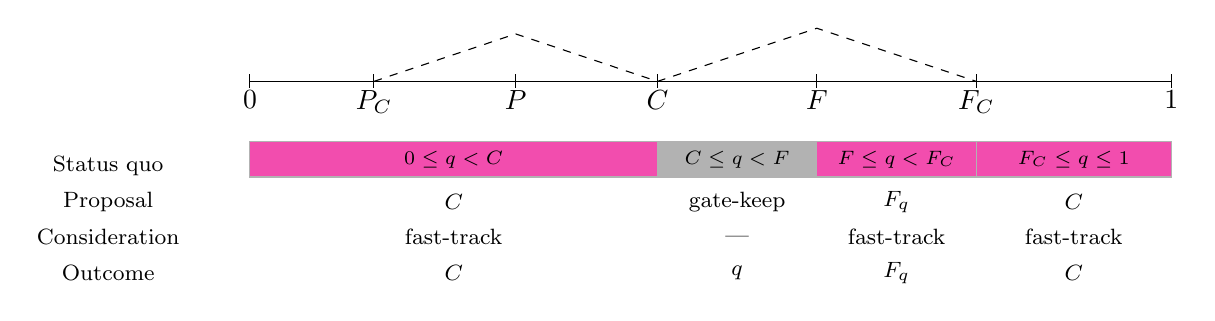
\begin{tikzpicture}[scale=.9]
          \draw (0,0) -- (13,0);% node[right] {$q \in X$};
          \draw[dashed] (1.75,0) -- (3.75,0.67) -- (5.75,0);
          \draw[dashed] (5.75,0) -- (8,.75) -- (10.25,0);
          \draw (0,0.1) -- (0,-0.1) node[below=-0.1] {$0$}
          (1.75,0.1) -- (1.75,-0.1) node[below=-0.1] {$P_C$}
          (3.75,0.1) -- (3.75,-0.1) node[below=-0.1] {$P$}
          (5.75,0.1) -- (5.75,-0.1) node[below=-0.1] {$C$}
          (8,0.1) -- (8,-0.1) node[below=-0.1] {$F$}
          (10.25,0.1) -- (10.25,-0.1) node[below=-0.1] {$F_C$}
          (13,0.1) -- (13,-0.1) node[below=-0.1] {$1$};
          \node at (-2,-2.7) {\footnotesize{Outcome}};
          \node at (-2,-2.2) {\footnotesize{Consideration}};
          \node at (-2,-1.7)  {\footnotesize{Proposal}};
          \node at (-2,-1.2)  {\footnotesize{Status quo}};
          \node at (2.875,-2.7)   {\footnotesize{$C$}};          % Outcome      
          \node at (2.875,-2.2) {\footnotesize{fast-track}};         % Consideration
          \node at (2.875,-1.7)   {\footnotesize{$C$}};          % Proposal     
          \node at (6.875,-2.7)   {\footnotesize{$q$}};        % Outcome      
          \node at (6.875,-2.2) {\footnotesize{---}};            % Consideration
          \node at (6.875,-1.7)   {\footnotesize{gate-keep}};     % Proposal     
          \node at (9.125,-2.7)   {\footnotesize{$F_q$}};        % Outcome      
          \node at (9.125,-2.2) {\footnotesize{fast-track}};         % Consideration
          \node at (9.125,-1.7)   {\footnotesize{$F_q$}};        % Proposal     
          \node at (11.625,-2.7)   {\footnotesize{$C$}};          % Outcome      
          \node at (11.625,-2.2) {\footnotesize{fast-track}};         % Consideration
          \node at (11.625,-1.7)   {\footnotesize{$C$}};          % Proposal     
          \filldraw[fill=magenta!70,draw=black!30]   (0,-1.35) rectangle node {\scriptsize{$0 \leq q < C$}} (5.75,-0.85);
          \filldraw[fill=black!30,draw=black!30]  (5.75,-1.35) rectangle node {\scriptsize{$C \leq q < F$}} (8,-0.85);
          \filldraw[fill=magenta!70,draw=black!30]  (8,-1.35) rectangle node {\scriptsize{$F \leq q < F_C$}} (10.25,-0.85);
          \filldraw[fill=magenta!70,draw=black!30]  (10.25,-1.35) rectangle node {\scriptsize{$F_C \leq q \leq 1$}} (13,-0.85);
          %% \filldraw[fill=black!50,draw=black!30]   (0,-1.35) rectangle node {\scriptsize{$0 \leq q < C$}} (5.75,-0.85);
          %% \filldraw[fill=black!30,draw=black!30]  (5.75,-1.35) rectangle node {\scriptsize{$C \leq q < F$}} (8,-0.85);
          %% \filldraw[fill=black!50,draw=black!30]  (8,-1.35) rectangle node {\scriptsize{$F \leq q < F_C$}} (10.25,-0.85);
          %% \filldraw[fill=black!50,draw=black!30]  (10.25,-1.35) rectangle node {\scriptsize{$F_C \leq q \leq 1$}} (13,-0.85);
        \end{tikzpicture} \\ \\

        \textbf{II. Moderate president profile:} $C \leq P \leq F$ \\ 
        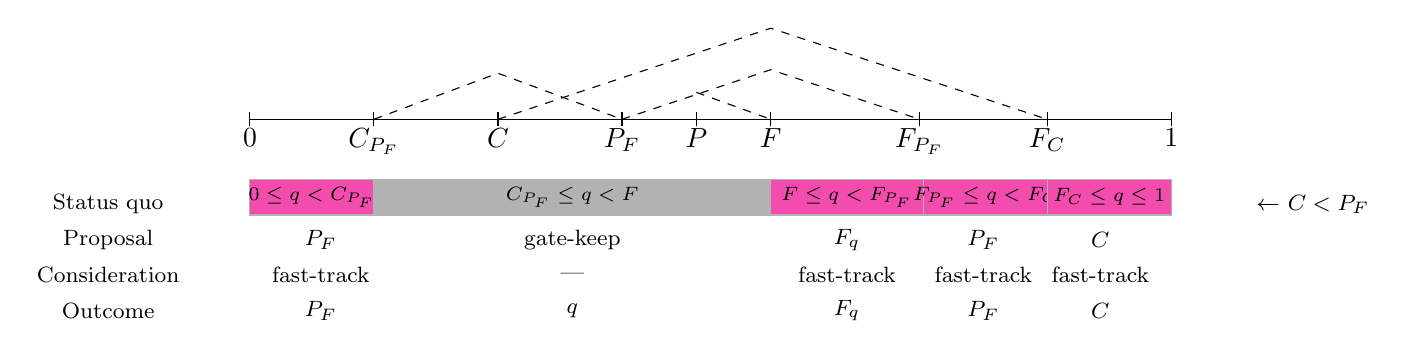
\begin{tikzpicture}[scale=.9]
          \draw (0,0) -- (13,0);% node[right] {$q \in X$};
          \draw[dashed] (1.75,0) -- (3.5,0.65) -- (5.25,0);
          \draw[dashed] (3.5,0) -- (7.35,1.285) -- (11.25,0);
          \draw[dashed] (5.25,0) -- (7.35,.7) -- (9.45,0);
          \draw[dashed] (6.3,0.38) -- (7.35,0);
          \draw (0,0.1) -- (0,-0.1) node[below=-0.1] {$0$}
          (1.75,0.1) -- (1.75,-0.1) node[below=-0.1] {$C_{P_F}$}
          (3.5,0.1) -- (3.5,-0.1) node[below=-0.1] {$C$}
          (5.25,0.1) -- (5.25,-0.1) node[below=-0.1] {$P_F$}
          (6.3,0.1) -- (6.3,-0.1) node[below=-0.1] {$P$}
          (7.35,0.1) -- (7.35,-0.1) node[below=-0.1] {$F$}
          (9.45,0.1) -- (9.45,-0.1) node[below=-0.1] {$F_{P_F}$}
          (11.25,0.1) -- (11.25,-0.1) node[below=-0.1] {$F_C$}
          (13,0.1) -- (13,-0.1) node[below=-0.1] {$1$};
          \node at (-2,-2.7) {\footnotesize{Outcome}};
          \node at (-2,-2.2) {\footnotesize{Consideration}};
          \node at (-2,-1.7)  {\footnotesize{Proposal}};
          \node at (-2,-1.2)  {\footnotesize{Status quo}};
          \node at (15,-1.2)  {\footnotesize{$\leftarrow$ $C<P_F$}};
          \node at (1,-2.7)   {\footnotesize{$P_F$}};           % Outcome      
          \node at (1,-2.2) {\footnotesize{fast-track}};            % Consideration
          \node at (1,-1.7)   {\footnotesize{$P_F$}};           % Proposal     
          \node at (4.55,-2.7)   {\footnotesize{$q$}};           % Outcome      
          \node at (4.55,-2.2) {\footnotesize{---}};               % Consideration
          \node at (4.55,-1.7)   {\footnotesize{gate-keep}};        % Proposal     
          \node at (8.425,-2.7)   {\footnotesize{$F_q$}};           % Outcome      
          \node at (8.425,-2.2) {\footnotesize{fast-track}};            % Consideration
          \node at (8.425,-1.7)   {\footnotesize{$F_q$}};           % Proposal     
          \node at (10.35,-2.7)   {\footnotesize{$P_F$}};           % Outcome      
          \node at (10.35,-2.2) {\footnotesize{fast-track}};            % Consideration
          \node at (10.35,-1.7)   {\footnotesize{$P_F$}};           % Proposal     
          \node at (12,-2.7)   {\footnotesize{$C$}};             % Outcome      
          \node at (12,-2.2) {\footnotesize{fast-track}};            % Consideration
          \node at (12,-1.7)   {\footnotesize{$C$}};             % Proposal     
          \filldraw[fill=magenta!70,draw=black!30]   (0,-1.35) rectangle node {\scriptsize{$0 \leq q < C_{P_F}$}} (1.75,-0.85);
          \filldraw[fill=black!30,draw=black!30]  (1.75,-1.35) rectangle node {\scriptsize{$C_{P_F} \leq q < F$}} (7.35,-0.85);
          \filldraw[fill=magenta!70,draw=black!30]  (7.35,-1.35) rectangle node {\scriptsize{$F \leq q < F_{P_F}$}} (9.5,-0.85);
          \filldraw[fill=magenta!70,draw=black!30]  (9.5,-1.35) rectangle node {\scriptsize{$F_{P_F} \leq q < F_C$}} (11.25,-0.85);
          \filldraw[fill=magenta!70,draw=black!30]  (11.25,-1.35) rectangle node {\scriptsize{$F_C \leq q \leq 1$}} (13,-0.85);
          %% \filldraw[fill=black!50,draw=black!30]   (0,-1.35) rectangle node {\scriptsize{$0 \leq q < C_{P_F}$}} (1.75,-0.85);
          %% \filldraw[fill=black!30,draw=black!30]  (1.75,-1.35) rectangle node {\scriptsize{$C_{P_F} \leq q < F$}} (7.35,-0.85);
          %% \filldraw[fill=black!50,draw=black!30]  (7.35,-1.35) rectangle node {\scriptsize{$F \leq q < F_{P_F}$}} (9.5,-0.85);
          %% \filldraw[fill=black!50,draw=black!30]  (9.5,-1.35) rectangle node {\scriptsize{$F_{P_F} \leq q < F_C$}} (11.25,-0.85);
          %% \filldraw[fill=black!50,draw=black!30]  (11.25,-1.35) rectangle node {\scriptsize{$F_C \leq q \leq 1$}} (13,-0.85);
        \end{tikzpicture} \\ \\

        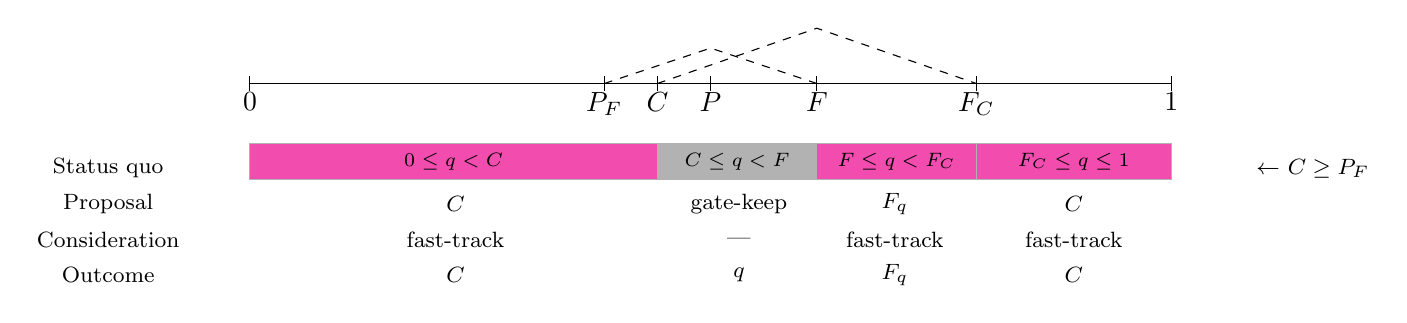
\begin{tikzpicture}[scale=.9]
          \draw (0,0) -- (13,0);% node[right] {$q \in X$};
          \draw[dashed] (5,0) -- (6.5,0.5) -- (8,0);
          \draw[dashed] (5.75,0) -- (8,.78) -- (10.25,0);
          \draw (0,0.1) -- (0,-0.1) node[below=-0.1] {$0$}
          (5,0.1) -- (5,-0.1) node[below=-0.1] {$P_F$}
          (5.75,0.1) -- (5.75,-0.1) node[below=-0.1] {$C$}
          (6.5,0.1) -- (6.5,-0.1) node[below=-0.1] {$P$}
          (8,0.1) -- (8,-0.1) node[below=-0.1] {$F$}
          (10.25,0.1) -- (10.25,-0.1) node[below=-0.1] {$F_C$}
          (13,0.1) -- (13,-0.1) node[below=-0.1] {$1$};
          \node at (-2,-2.7) {\footnotesize{Outcome}};
          \node at (-2,-2.2) {\footnotesize{Consideration}};
          \node at (-2,-1.7)  {\footnotesize{Proposal}};
          \node at (-2,-1.2)  {\footnotesize{Status quo}};
          \node at (15,-1.2)  {\footnotesize{$\leftarrow$ $C \geq P_F$}};
          \node at (2.9,-2.7)   {\footnotesize{$C$}};        % Outcome      
          \node at (2.9,-2.2) {\footnotesize{fast-track}};       % Consideration
          \node at (2.9,-1.7)   {\footnotesize{$C$}};        % Proposal     
          \node at (6.9,-2.7)   {\footnotesize{$q$}};      % Outcome      
          \node at (6.9,-2.2) {\footnotesize{---}};          % Consideration
          \node at (6.9,-1.7)   {\footnotesize{gate-keep}};   % Proposal     
          \node at (9.1,-2.7)   {\footnotesize{$F_q$}};      % Outcome      
          \node at (9.1,-2.2) {\footnotesize{fast-track}};       % Consideration
          \node at (9.1,-1.7)   {\footnotesize{$F_q$}};      % Proposal     
          \node at (11.625,-2.7)   {\footnotesize{$C$}};         % Outcome      
          \node at (11.626,-2.2) {\footnotesize{fast-track}};        % Consideration
          \node at (11.625,-1.7)   {\footnotesize{$C$}};         % Proposal     
          \filldraw[fill=magenta!70,draw=black!30]   (0,-1.35) rectangle node {\scriptsize{$0 \leq q < C$}} (5.75,-0.85);
          \filldraw[fill=black!30,draw=black!30]  (5.75,-1.35) rectangle node {\scriptsize{$C \leq q < F$}} (8,-0.85);
          \filldraw[fill=magenta!70,draw=black!30]  (8,-1.35) rectangle node {\scriptsize{$F \leq q < F_C$}} (10.25,-0.85);
          \filldraw[fill=magenta!70,draw=black!30]  (10.25,-1.35) rectangle node {\scriptsize{$F_C \leq q \leq 1$}} (13,-0.85);
          %% \filldraw[fill=black!50,draw=black!30]   (0,-1.35) rectangle node {\scriptsize{$0 \leq q < C$}} (5.75,-0.85);
          %% \filldraw[fill=black!30,draw=black!30]  (5.75,-1.35) rectangle node {\scriptsize{$C \leq q < F$}} (8,-0.85);
          %% \filldraw[fill=black!50,draw=black!30]  (8,-1.35) rectangle node {\scriptsize{$F \leq q < F_C$}} (10.25,-0.85);
          %% \filldraw[fill=black!50,draw=black!30]  (10.25,-1.35) rectangle node {\scriptsize{$F_C \leq q \leq 1$}} (13,-0.85);
        \end{tikzpicture} \\ \\

        \textbf{III. Moderate floor profile:} $C <  F <  P$ \\ 
        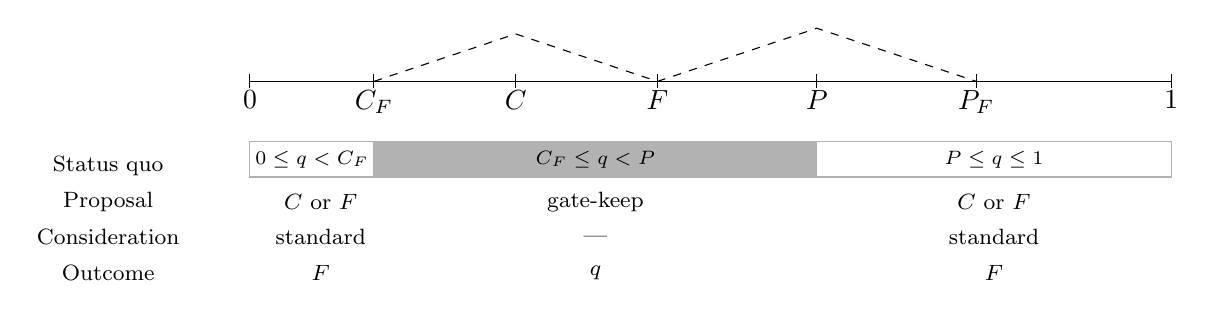
\begin{tikzpicture}[scale=.9]
          \draw (0,0) -- (13,0);% node[right] {$q \in X$};
          \draw[dashed] (1.75,0) -- (3.75,0.67) -- (5.75,0);
          \draw[dashed] (5.75,0) -- (8,.75) -- (10.25,0);
          \draw (0,0.1) -- (0,-0.1) node[below=-0.1] {$0$}
          (1.75,0.1) -- (1.75,-0.1) node[below=-0.1] {$C_F$}
          (3.75,0.1) -- (3.75,-0.1) node[below=-0.1] {$C$}
          (5.75,0.1) -- (5.75,-0.1) node[below=-0.1] {$F$}
          (8,0.1) -- (8,-0.1) node[below=-0.1] {$P$}
          (10.25,0.1) -- (10.25,-0.1) node[below=-0.1] {$P_F$}
          (13,0.1) -- (13,-0.1) node[below=-0.1] {$1$};
          \node at (-2,-2.7) {\footnotesize{Outcome}};
          \node at (-2,-2.2) {\footnotesize{Consideration}};
          \node at (-2,-1.7)  {\footnotesize{Proposal}};
          \node at (-2,-1.2)  {\footnotesize{Status quo}};
          %\node at (15,-1.2)  {\footnotesize{$\leftarrow$ veto will}};
          %\node at (15,-1.7)  {\footnotesize{be overridden}};
          \node at (1,-2.7)   {\footnotesize{$F$}};              % Outcome      
          \node at (1,-2.2) {\footnotesize{standard}};           % Consideration
          \node at (1,-1.7)   {\footnotesize{$C$ or $F$}};              % Proposal     
          \node at (4.875,-2.7)   {\footnotesize{$q$}};         % Outcome      
          \node at (4.875,-2.2) {\footnotesize{---}};             % Consideration
          \node at (4.875,-1.7)   {\footnotesize{gate-keep}};      % Proposal     
          \node at (10.5,-2.7)   {\footnotesize{$F$}};          % Outcome      
          \node at (10.5,-2.2) {\footnotesize{standard}};       % Consideration
          \node at (10.5,-1.7)   {\footnotesize{$C$ or $F$}};   % Proposal     
          \filldraw[fill=black!0,draw=black!30]   (0,-1.35) rectangle node {\scriptsize{$0 \leq q < C_F$}} (1.75,-0.85);
          \filldraw[fill=black!30,draw=black!30]  (1.75,-1.35) rectangle node {\scriptsize{$C_F \leq q < P$}} (8,-0.85);
          \filldraw[fill=black!0,draw=black!30]  (8,-1.35) rectangle node {\scriptsize{$P \leq q \leq 1$}} (13,-0.85);
          %% \filldraw[fill=black!0,draw=black!30]   (0,-1.35) rectangle node {\scriptsize{$0 \leq q < C_F$}} (1.75,-0.85);
          %% \filldraw[fill=black!30,draw=black!30]  (1.75,-1.35) rectangle node {\scriptsize{$C_F \leq q < P$}} (8,-0.85);
          %% \filldraw[fill=black!0,draw=black!30]  (8,-1.35) rectangle node {\scriptsize{$P \leq q \leq 1$}} (13,-0.85);
        \end{tikzpicture} \\ \\

      \end{tabular}
    }
\end{figure}

Under what conditions will presidents fast-track legislation? And what conditions will make them willing to allow for open rules? To answer, and by so doing derive empirical implications, we extend the bargaining logic across preference profiles. A preference profile is an ordering of players' ideal points in space. Three profiles are portrayed in Figure \ref{F:predictions}, distinguishing which player is moderate relative to the others: the committee ($P<C<F$), the president ($C \leq P \leq F$), and the floor ($C<F<P$); the other mutually-exclusive and exhaustive profiles are mirror-images. The example from Figure 2 belongs in the moderate committee profile I, but we now treat the status quo as a variable $q \in [0,1]$---the example's is in $0 \leq q < C$. The figure traces how changes in $q$ affect three measures of interest: the proposal, the consideration regime, and the game's outcome. Each discrete zone (the pink, gray, or white rectangles) keeps status quos with unchanging equilibrium components together.

%It is plain in the figure that white rectangles, corresponding to standard bill consideration, occur under the moderate floor profile only. So a profile like I or II (where president and committee ideal points lie on the same side of the floor median), but not III (where they lie on either side), is a necessary condition for urgent consideration. While the condition is readily visible in theory, ideal point unobservability is an obstacle towards a test. We surmount it with the help of auxiliary assumptions: that chairs are dictators in committee proceedings; and that players sharing a party label have more proximal ideal points than those of different parties.\footnote{Derivation involves the more technical auxiliary assumption of a stochastic status quo whose probability distibution has support in $[0,1]$---i.e., $q$ occurs in any range of the policy space with non-zero probability. Dropping it creates discontinuities in prediction, which complicate exposition. See \citet[:38]{cox.mccubbins.2005} for an elaboration.} By the first, committee are unitary actors. The other associates player preferences to something observable. Standing orders (see footnote \ref{fn:comm-chains}) and party discipline \citep{aleman.saiegh.coalUnityChile.2007,carey.2002} lend support for auxiliary assumptions in Chile. The next prediction follows. 

The first thing to notice is that fast-track occurs only when the president and committee ideal points lie on the same side of the floor median (i.e., a profile other than the moderate floor is a necessary condition for the fast track). We assume that committees are unitary actors where chairs are dictators; and that players from the same party have closer ideal points than players from different parties.\footnote{House rules in Chile (see footnote \ref{fn:comm-chains}) and party discipline \citep{aleman.saiegh.coalUnityChile.2007,carey.2002} support these assumption in the Chilean case. Derivation involves the more technical auxiliary assumption of a stochastic status quo whose probability distibution has support in $[0,1]$---i.e., $q$ occurs in any range of the policy space with non-zero probability. Dropping it creates discontinuities in prediction, which complicate exposition. See \citet[:38]{cox.mccubbins.2005} for an elaboration.} Thus, the results show that when the committee chair and the president have close preferences relative to the floor---that is, when they lie on the same side of $F$---the bill coming out from committee will be considered under urgent procedures. 

In other words, when the president and the committee chair belong to the same party, they will be able to negotiate a bill that is acceptable to both of them. Under such circumstances, the president will have an incentive to declare the bill urgent so she can prevent floor amendmets that would otherwise move the bill further away. The president does not utilize the urgency to accelerate bill approval, but instead uses it to protect the bill from unwanted amendments on the floor. In this sense, the president takes on the role of the Rules Committee, deciding whether the bill will reach the floor under closed or open rules. Our first hypothesis reflects the conditions under which the president will use her urgency authority.

%\begin{description}
%  \item [Hypothesis:] Other things constant, a fast-track is no less probable when the reporting committee's chair %belongs to the president's party than when president and committee chair belong to different parties. 
%\end{description}

\begin{description}
  \item [Hypothesis 1:] Presidents are more likely to fast-track bills when the committee chair with jurisdiction over the bill  belongs to the president's party than otherwise.
\end{description}

%The wording is `no less probable' due to a necessary but insufficient condition (see the Appendix). 

The hypothesis is not independent of the location of floor preferences with respect to the president, and clearly, when floor preferences are closer to the president than the preferences of the committee chair, the necessity to fast track bills declines. To see this, hold the distance separating $P$ and $F$ constant while shrinking the distance between $C$ and $P$ and see what happens in each profile. Magenta rectangles become more prominent relative to gray ones in I and II (the probability of the fast-track goes up) but not in III (where the fast-track probability remains unchanged). 
%I see III as the profile in which the F and P are proximate while C is in hands of the opposition, hence in line with our hypothesis.

The other important result refers to the conditions under which the president will decide not to use her urgency authority.  Figure \ref{F:predictions} shows that standard bill consideration (white rectangles) occurs under the moderate floor profile only, when committee and president are on either side of the floor median. This means that when the preferences of the committee and the president are farther apart---i.e., they belong to different parties---the president will not get in the way of open rule consideration of bills. By allowing amendments, which bring policy towards $F$, the president will be able to move the bill closer to her ideal point. Thus, if a committee chair belongs to an opposition party, the president has the power to influence bills by allowing the regular procedure (open rule) to operate, that is, by desisting from using her urgency authority. Thus, our second hypothesis refers to the conditions under which the president will refrain from fast-tracking bills.\footnote{Empirical implications about other measures of interest, such as gatekeeping and expected bargaining outcomes, also follow from models in the spatial family. We did not systematize data from bill histories to test these implications, so we do not discuss them here.} 

\begin{description}
  \item [Hypothesis 2:] Presidents are more likely to allow open rule consideration of bills when the committee chair with jurisdiction over the bill belongs to a party that is not in the president's coalition than otherwise.
\end{description}

We replace `party' with `coalition' as alternative measure of preferences in the test. Chilean politics since 1990 has operated under the coalition logic. Two main coalitions, one from the center-right and the other from the center-left, work cohesively in government and in the opposition. Coalition discipline is well-documented \citep{carey.2002,aleman.saiegh.coalUnityChile.2007}. 


\section{Data and Analysis}

We collected original data to test the hypothesis, compiling bill histories of every draft law that the executive introduced in Congress between 1998 and 2014:\footnote{We scraped the \emph{Cámara de Diputados'} web page (\url{www.camara.cl}) in November 2014 to retrieve the record (\emph{boletín}) of every proposal made between 11 March 1998 and 10 March 2014, inclusive. Data and commented code for replication accompany the on-line appendix. We conducted data analysis with a multiplicity of \texttt{R}'s libraries.} when each was introduced, in which chamber of the bicameral Congress, the issue it deals with, the status at the time of consultation, and so forth. We also gathered information on the chronological detail of the bill's legislative process in the House: committee referrals and reports, floor discussion and voting, navette to the Senate, and more. Of direct relevance, we coded all bills marked urgent in the \emph{Cámara de Diputados}. Earlier years antedate Internet publication and were dropped, as data completeness in the primary source remains to be verified. The period selected fully covers two Senates, four \emph{Cámaras}, and three presidencies (plus the last two years of an earlier presidency).

%% EMM [13jun18] He quitado los tres párrafos siguientes. Si lo piden los referees, podemos retomar parte o todo.

%% The Chilean Constitution of 1980 sets the institutional order allocating decision rights across the branches in Chile. Presidents are elected for four-year terms and immediate reelection is forbidden. Legislators in the period were elected through direct elections in two-member districts. Its 120 lower house representatives are elected for four-year terms, while the thirty-eight senators serve eight-year terms. Parties in Congress organized in two stable coalitions, the center-left Concertación (later Nueva Mayoría), and the center-right Alianza (later Chile Vamos). 

%% Chilean presidents concentrate considerable legislative power \citep[][, Payne 2006, Author 2017]{baldez.carey.1999,siavelis.2002}. Their prerogatives include exclusive proposal power in key legislative areas such as all new spending, finance, and administration. The president can affect the congressional agenda by marking bills urgent, which imposes time constraints on their discussion. She can also propose amendments to bills under consideration. In the twenty-four years between the return to democracy and the end of Piñera’s administration in 2014, a total of 8,483 bills were proposed. The Chilean congress passed 2,617 of those bills (approximately one third). Most of these bills had been marked urgent at some point of their life span, and defying commom sense, some were marked urgent several times. 

%% However, counter mainstream expectations that more powerful presidents use their prerogatives more broadly \citep{odonnell.1993,odonnell.1994}, Chilean politics function in a consensual manner and presidents rarely use their more confrontational prerogatives, such as decrees and total vetoes. As other Latin American presidents, the Chilean president can enact legislation by decree, what Shugart and Carey (1998) term Constitutional Decree Authority. However, between 1990 and 2014 only two decrees were enacted in Chile, as opposed to hundreds enacted in Argentina (694 between 1983 and 2007) and Brazil (744 between 1988 and 2010). This paper assumes that consensual behavior is crafted through institutional procedures. Understanding which procedures are key in this regard is part of this paper's contribution. %It sets out to understand the conditions under which presidents can move along their agendas while maintaining politics consensual. 

% numbers produced in chillBill.r (above xtable command). Verify if changes have occurred since...
\begin{table}
\centering
\caption{Proposals, legislation, and fast-track authority}\label{T:billDescriptives}
\begin{tabular}{llrr}
\multicolumn{4}{c}{\textbf{Part A. Executive bills}} \\
   & \multicolumn{2}{l}{Bills}                           &   frequency  \\ \hline
I  & \multicolumn{2}{l}{introduced}                      &       1,467  \\ \hdashline
II & \multicolumn{2}{l}{passed}                          &       1,059  \\
   & \multicolumn{2}{l}{as \% of introduced}             &   \emph{72}  \\ \hdashline
III& \multicolumn{2}{l}{fast-tracked}                    &         540  \\
   & \multicolumn{2}{l}{as \% of introduced}             &   \emph{37}  \\ \hdashline
IV & \multicolumn{2}{l}{fast-tracked \& passed}          &         415  \\
   & \multicolumn{2}{l}{as \% of fast-tracked}           &   \emph{77}  \\ \hline
\\
\multicolumn{4}{c}{\textbf{Part B. Urgent bills by presidency}} \\
\multicolumn{2}{l}{President and period}    & $N$ bills & \% fast-tracked \\ \hline
\multicolumn{2}{l}{Frei 1998--2000$^\dagger$} & 128       &  \emph{38} \\
\multicolumn{2}{l}{Lagos 2000--2006}        & 544       &  \emph{25} \\
\multicolumn{2}{l}{Bachelet 2006--2010}     & 392       &  \emph{39} \\
\multicolumn{2}{l}{Piñera 2010--2014}       & 403       &  \emph{50} \\ \hdashline
\multicolumn{2}{l}{All 1998--2014}          & 1,467     &  \emph{37} \\
\hline
\multicolumn{4}{r}{\footnotesize{$^\dagger$ Last third of the six-year term in the analysis only.}} \\
\end{tabular}
\end{table}

Table \ref{T:billDescriptives} offers a general summary of bill introduction, passage, and fast-track incidence. The executive sent 1,467 bills to Congress between 1998 and 2014, ninety-one yearly on average. (Members of Congress proposed 79 percent of all bills, not analyzed.) More than one thousand proposals became law during the period, putting the executive's success rate at 72 percent---high by Latin American standards \citep{morgenstern.nacif.2002}. And 540 bills were on the fast-track during lower chamber consideration, 37 percent of all bills introduced. And 77 percent of those became law, so about 40 percent of bills that became law did it under restrictive procedures. 

The variance in urgency incidence across administrations, reported in part B, is considerable. But differences in urgency authority usage do not seem related with specifics traits of the president. For instace, one could argue that presidents with previous legislative experience might be less inclined to interfere with Congressional priorities. Frei (with previous legislative experience) and Bachelet (without) were about on average, Lagos (with experience) quite below, and Piñera (without) quite above. %Might experience color President Frei's attitude towards urgency authority upon returning to Congress afterwards? We unfortunately could find no record of this in the press.

\subsection{Fast-track predictors}

Multivariate analysis of the data is revealing. The units of analysis are individual executive proposals: the dependent variable \emph{Fast-tracked Bill} equals 1 for proposals marked with `supreme urgency' while in the Cámara, 0 otherwise. Our main independent variable accounts for preference coincidence between the president and the reporting committee. We include controls for bill features, for timing, and for the strategic environment. Formal variable definitions and descriptive statistics appear in the appendix.

With respect to our main independent variable, which accounts for preferences, we include \emph{Co-partisan Chair} and \emph{Coalition Chair}, which seek to identify committee chairs' preference location vis-\`a-vis the president, and \emph{Multiple Referrals}, which identifies bills referred to multiple committees. \emph{Co-partisan Chair} equals 1 if the bill was referred to a standing committee presided by a member of the president's party, and equals 0 otherwise; \emph{Coalition Chair} equals 1 for bills referred to committees chaired by members of any party in the presidential coalition, 0 otherwise. These are two different ways in which we measure our key explanatory variable, spatial proximity between the chief executive and the reporting committee, and we expect each to associate positively with the dependent variable. Part A of Table \ref{T:chairsSeats} shows that the number of standing committee chairs in hands of the president's party varied in the period, from a high of 53 percent in the 1998--2002 legislature to a low of 17 percent in 2006--10. And the opposition chaired no standing committee in 2006--10, but up to 24 and 27 percent in 2002--06 and 2010--14, respectively.\footnote{\emph{Largesse} towards opposition parties was probably aimed at beefing up the president's legislative support. Unlike the Senate, the coalition remained in control of the Cámara throughout the period. But, by requiring 67, 60, and 57 percent votes of each chamber, respectively, constitutional reform, constitution-interpreting legislation, and organic laws therefore always required support across the aisle.}

%\textbf{NOTE:IN THIS PARAGRAPH, I GUESS, WE SHOULD EXPLAIN VARIABLE USED TO TEST HYP2 (WHICH WILL POSSIBLY BE THE COMPLEMENT OF COALITION CHAIR, BUT NOT SURE WHAT TO DO ABOUT INDEPENDENTS, ID SAY THEY ARE NOT IN THE COALITION IN ANY CASE, ALTHOUGH THEY HAVE SYSTEMATICALLY SUPPORTED THE RIGHT.} 

\begin{table}
\centering
\caption{The president's status in Congress and its committees. Percent chairs/seats by party. The president's coalition in 1998--2010 was Concertación; it was Alianza afterwards. Regional includes major-party splinters (from Christian Democrats and UDI). President's status in the Senate slightly and briefly oscillated above and below majority due to vacant seats. Source: prepared with information from \protect\url{www.camara.cl}.}\label{T:chairsSeats}
\begin{tabular}{lrrrr}
                      & 1998--2002 & 2002--06 & 2006--10 & 2010--14 \\ \hline
\mc{5}{c}{\textbf{~~Part A. Committee chairs, Cámara}} \\
President's party     &  \emph{53} & \emph{35}  & \emph{17}  & \emph{23}   \\
Other coalition party &  \emph{41} & \emph{41}  & \emph{83}  & \emph{50}   \\
Opposition            &   \emph{6} & \emph{24}  &            & \emph{27}   \\ \hdashline
Total                 & \emph{100} & \emph{100} & \emph{100} & \emph{100}  \\ 
$N$ standing committees&  17        &  17      &  18      & 22      \\ [1.8ex] \hline 
\mc{5}{c}{\textbf{~~Part B. Seats, Cámara}} \\ 
President's coalition & \emph{58}     & \emph{53}  & \emph{51}   & \emph{50}   \\
Opposition            & \emph{42}     & \emph{48}  & \emph{47}   & \emph{48}   \\
Regional              &               &            & \emph{3}    & \emph{2}    \\ \hdashline
Total       & \emph{100}    & \emph{100} & \emph{100}  & \emph{100}  \\ [1.8ex] \hline
\mc{5}{c}{\textbf{~~Part C. Seats, Senate}} \\
President's coalition & \emph{50}            & \emph{50}       & \emph{55}   & \emph{45}       \\
Opposition            & \emph{50}            & \emph{50}       & \emph{45}   & \emph{55}       \\ \hdashline
Total                 & \emph{100}$^{\dagger}$ & \emph{100}      & \emph{100}  & \emph{100}      \\ \hline
\mc{5}{r}{\footnotesize{$^\dagger$vacant seats dropped}}
\end{tabular}
% \begin{tabular}{lrrrrrr}
% Coalition   & 1990--94 & 1994--98 & 1998--2002    & 2002--06 & 2006--10 & 2010--14 \\ \hline
% \mc{7}{l}{\emph{~~Cámara de Diputados}} \\
% President's & 60       & 58       & 58            & 53       & 51       & 50       \\
% Opposition  & 40       & 42       & 42            & 48       & 47       & 48       \\
% Regional    &          &          &               &          & 3        & 2        \\ \hdashline
% Total       & 100      & 100      & 100           & 100      & 100      & 100      \\ \hline
% \mc{7}{l}{\emph{~~Senate}} \\
% President's & 48       & 46       & 50            & 50       & 55       & 45       \\
% Opposition  & 52       & 54       & 50            & 50       & 45       & 55       \\ \hdashline
% Total       & $100^*$  & $100^*$  & $100^{*\dagger}$ & 100      & 100      & 100      \\ \hline
% \mc{7}{l}{\footnotesize{Notes: $^*$ vacant seats dropped; $^\dagger$ margin varied above and below 50/50 due to vacancies.}}
% \end{tabular}
\end{table}

We also control for multiple referrals. Nearly one quarter (24 percent) of bills in the period were referred to more than one standing committee. The `other committee' count excludes the Finance Committee, with jurisdiction over any form of new spending (and discussed next---multiple referrals reach 32 percent when the Finance Committee is considered). Also excluded are special and bicameral committees. \emph{Multiple Referrals} should capture any effect of agenda control sharing among several committee chairs during the proposal's negotiation---reflecting the need to rein on unruly chairs through a friendlier committee. A single co-partisan or coalition chair among multiple referees suffices for the indicator previously discussed to equal 1. 

The variable intended to capture bill-specific features is \emph{Hacienda Referral}, which equals 1 for bills referred to the powerful Finance Committee with special status in the Chilean Congress, 0 otherwise. Unlike other standing committees, Finance has jurisdiction over \emph{every} bill authorizing spending in any domain. Moreover, the unanimous exception rule discussed earlier is inapplicable to \emph{Hacienda} bills, which must be reported prior to floor consideration.\footnote{\emph{Ley Orgánica del Congreso} arts.\ 17 and 21.} Committee members, working in tandem with the Finance Ministry, may or may not appropriate funds from the budget in their report \citep{aleman.navia.UrgChi.2009}. Not unlike the Appropriations and Rules committees in the U.S.\ House, \emph{Hacienda} has the status of a control committee, a key asset for agenda power \citep{kiewiet.mccubbins.1991}. \emph{Hacienda} referral therefore controls for a subset of generally important proposals, and we expect it to associate positively with urgency authority.
%So, for instance, a proposal restricting labor benefits to municipal health workers was referred to both the Public Health and Hacienda committees because a small appropriation for verification by the Labor Bureau was \todo{Find another bill to illustrate... can't find date and other elements of the mentioned law} required. 

Three controls account for the strategic environment. \emph{Presidential Approval} is the net general population presidential approval rate at bill initiation (i.e., the percentage of respondents who approve of the president's job minus the percentage who disapprove). We have no a priori expectation here. If presidents with better public opinion standing are also more successful in the legislative arena \citep{bond.fleisher.1990,aleman.navia.UrgChi.2009}, they might also need restrictive rules less often, and reliance on the fast-track might therefore drop (in some issue areas, at least).\footnote{We estimate the models using subsets of bills by issue area in the on-line appendix. Smaller numbers of bills tend to hamper statistical significance, but the results are in line with those reported.} The contrary might hold if popular presidents were more successful in obtaining more likeable reports from the average committee chair, that would then require protection against floor amendments. \emph{Introduced in Senate} equals 1 for bills sent to the Upper Chamber, 0 otherwise. By virtue of being smaller, enjoying longer terms, and not being firmly under the president's coalition control during most of the period, bills sent to the Senate might present systematic differences in fast-track usage. And \emph{Senate Majority} equals 1 if the president's coalition controlled half or more of Upper Chamber seats when the bill was initiated, 0 otherwise.\footnote{Parties in the presidential and opposition coalitions were tied throughout most of the 1998--2006 Senate (majority briefly oscillating back and forth in the first years due to member indictments, impeachments, and deaths in both coalitions). Ties are coded as \emph{Senate Majority} = 1.} Other things equal, presidents with sufficient partisan legislative resources in both chambers will find it easier to push proposals through Congress, and might be less inclined to use the fast-track prerogative to successfully navigate log-rolls through the plenary session.

The group of variables accounting for time-related effects control for different aspects of the congressional cycle. \emph{Year Remaining} (and its squared value to capture non-linearity, if any) measures the percentage of the legislative year remaining at bill initiation. Chilean legislative years start after the (meridional) Summer break. So the variable adopts value 100 for proposals introduced on March 1 (the first day of the legislative year), and value 0 for proposals introduced the last day of February. It should control for stationarity in the data (the on-line appendix elaborates the temporal dimension in the use of urgencies). And \emph{Relax Deadline} equals 1 for bills initiated in July 2010 or later, 0 otherwise. Congress doubled deadlines to consider and vote urgent bills five months into the 2010--14 legislature (see Appendix). Any systematic shift in urgency usage attributable to this reform should reflect in this coefficient. 

\subsection{Model Specification and Results}

Given that we pool observations from four elected legislatures, with important differences in the types and the volume of proposals considered \citep{aleman.navia.UrgChi.2009}, heterogeneity might interfere. We fit two additional model specifications for robustness verification. One includes fixed legislature effects---i.e., three dummies for bills initiated in the 2002--06, 2006--10, and 2010--14 periods, respectively; the excluded 1998--2002 dummy is the baseline. Another adds further flexibility by also estimating separate errors for bills initiated in each legislature \citep[a so-called mixed effects model,][:262,302]{gelman.hill.2007}. We rely on a generalized linear model for mixed effects estimation, and logit for the rest. We normalized continuous variables \emph{Presidential Approval} and \emph{Year Remaining} to speed the GLM's convergence.\footnote{As suggested in \url{http://stackoverflow.com/questions/23478792/warning-messages-when-trying-to-run-glmer-in-r} and \url{https://rstudio-pubs-static.s3.amazonaws.com/33653_57fc7b8e5d484c909b615d8633c01d51.html}. Normalization re-scales and centers the measures in order to improve parameter identification.} Normalized measures were used throughout for model comparability.

% next command removes proportional font in table's superscripts
%(eval-after-load "tex-mode" '(fset 'tex-font-lock-suscript 'ignore)) 

% Table created by stargazer v.5.2 by Marek Hlavac, Harvard University. E-mail: hlavac at fas.harvard.edu
% Requires LaTeX packages: dcolumn 
\begin{table}%[!htbp]
  \centering 
  \caption{Executive bill fast-track predictors. Model 3 includes fixed Legislatura effects (not reported). Model 4 estimates separate error terms by Legislatura. Method of estimation: model 4 with generalized linear model, others with logit \citep[fitted with \texttt{R} base's \texttt{glm} and library \texttt{lme4},][]{lme4.2015}.}\label{t:urgenLogit}
  \begin{tabular}{@{\extracolsep{0pt}}lD{.}{.}{-3} D{.}{.}{-3} D{.}{.}{-3} D{.}{.}{-3} } 
    \hline \\[-1.8ex] 
    & \multicolumn{4}{c}{DV: Bill on fast-track (1) or not (0)} \\ 
    \\[-1.8ex] & \multicolumn{1}{c}{(1)} & \multicolumn{1}{c}{(2)} & \multicolumn{1}{c}{(3)} & \multicolumn{1}{c}{(4)}\\ 
    \\ [-1.8ex] 
    \hline \\[-1.8ex] 
    \emph{Co-partisan}     &  .289^{**}   &  &  &                                        \\
    \emph{Chair}           & (.024)      &  &  &                                             \\ [.75ex]
    \emph{Coalition}       &             & .825^{***}   & .874^{***}    & .847^{***}                 \\
    \emph{Chair}           &             & (.005)      & (<.001)     & (<.001)                             \\ [.75ex]
    \emph{Multiple}        &  .772^{***}  &  .795^{***}  &  .808^{***}   &  .809^{***}      \\
    \emph{Referrals}       & (<.001)     & (<.001)     & (<.001)     & (.004)                      \\ [.75ex]
    \emph{Hacienda}        & 1.002^{***}  & .940^{***}   & .917^{***}    & .923^{***}      \\
    \emph{Referral}        & (<.001)     & (<.001)     & (<.001)     & (<.001)                      \\ [.75ex]
    \emph{Pres.}           &  -.078      &  -.096      &  .029       & -.044                            \\
    \emph{Approval}        & (.286)      & (.187)      & (.710)      & (.567)                          \\ [.75ex]
    \emph{Introduced}      &  -.716^{***} &  -.698^{***}  &  -.744^{***} &  -.730^{***}  \\
    \emph{in Senate}       & (<.001)     & (<.001)     & (<.001)      & (<.001)                      \\ [.75ex]
    \emph{Senate}          &  -.251      &  -.319      &  &                                   \\
    \emph{Majority}        & (.214)      & (.110)      &  &                                       \\ [.75ex]
    \emph{Year}            &  .072       &  .065       &  .053        &  .053                              \\
    \emph{Remaining}       & (.223)      & (.268)      & (.370)       & (.368)                          \\ [.75ex]
    \emph{(Year}           &  -.224^{***} &  -.238^{***}  &  -.255^{***}  &  -.251^{***}  \\
    \emph{Remaining)$^2$}  & (<.001)     & (<.001)      & (<.001)      & (<.001)                      \\ [.75ex]
    \emph{Relax}           &  .479^{*}    &  .394       &  &                               \\
    \emph{Deadline}        & (.057)      & (.104)      &   &                                       \\ [.75ex]
    %% \emph{2002-06 Leg.} &  &  &  -.203 &                                             \\
    %%                     &  &  & (.298) &                                             \\ [.75ex]
    %% \emph{2006-10 Leg.} &  &  &  .302^{*} &                                          \\
    %%                     &  &  & (.097) &                                             \\ [.75ex]
    %% \emph{2010-14 Leg.} &  &  & 1.200^{***} &                                        \\
    %%                     &  &  & (<.001) &                                            \\ [.75ex]
    Intercept              &  -1.046^{***} & -1.589^{***} & -1.933^{***} & -1.719^{***}  \\
                           & (<.001)      & (<.001)     & (<.001)    & (<.001)                       \\ [.75ex]
    \hline \\[-1.8ex] 
    Effects & \multicolumn{1}{c}{none} & \multicolumn{1}{c}{none} & \multicolumn{1}{c}{fixed} & \multicolumn{1}{c}{mixed} \\ 
    Observations & \multicolumn{1}{c}{1,467} & \multicolumn{1}{c}{1,467} & \multicolumn{1}{c}{1,467} & \multicolumn{1}{c}{1,467} \\ 
    Log$L$ & \multicolumn{1}{c}{$-864$} & \multicolumn{1}{c}{$-862$} & \multicolumn{1}{c}{$-852$} & \multicolumn{1}{c}{$-859$} \\ 
    \% correct & \multicolumn{1}{c}{67} & \multicolumn{1}{c}{68} & \multicolumn{1}{c}{68} & \multicolumn{1}{c}{68} \\ 
%%Akaike Inf. Crit. & \multicolumn{1}{c}{1,748.896} & \multicolumn{1}{c}{1,740.400} & \multicolumn{1}{c}{1,719.057} & \multicolumn{1}{c}{1,731.050} \\ 
%%Bayesian Inf. Crit. &  &  &  & \multicolumn{1}{c}{1,778.632} \\ 
    \\ [-1.8ex] 
    \hline \\[-1.8ex] 
    & \multicolumn{4}{r}{\footnotesize $^{*}$p$<$.1; $^{**}$p$<$.05; $^{***}$p$<$.01 (p-values in parentheses)} \\ 
  \end{tabular} 
\end{table} 

%\emm{New model, includes executive bills only. Excludes urgency messages in Senate (previously conflated with Cámara urgencias). Could report member bills model in the appendix (coalition chair doesn't work, but co-partisan does!), but adds little to our argument---urgent member bills seem to respond to a different logic.}

Table \ref{t:urgenLogit} reports results.\footnote{The regression model performs satisfactorily. A likelihood-ratio test of overall fit rejects the hypothesis, at below the .001 level, that an intercept-only fit is as good as our models. Predictors across model specifications correctly classify 67--68 percent of the observations.} We find support for our main hypothesis. In line with expectations, both variables measuring the proximity of committee chairs to the president increase the probability of fast-track. \emph{Co-partisan Chair} has a positive coefficient in model 1, as hypothesized, and the effect achieves conventional statistical significance (parentheses in the table report p-values). The evidence is much stronger for the variable's other specification: the coefficient for \emph{Coalition Chair} in models 2--4 is also positive, triples its size, and achieves p-values at .005 or below. In other words, if a bill is referred to a committee where the president finds support (either because the chair belongs to her party or to her coalition), the report is more likely to be fast-tracked for floor consideration. This matches previous scholarship, i.e., that the coalition is as good a predictor of presidential support in Congress---or better, in our case---as the party. The finding is robust across model specifications. In general, all model coefficients remain pretty much unchanged in size and significance when fixed and mixed effects are included on the right side (\emph{Senate Majority} and \emph{Relax Deadline} must be dropped due to co-linearity with legislature dummies). 

%% > mar3
%%      factor     AME     SE       z      p   lower   upper
%%   dsameCoal  0.1734 0.0585  2.9651 0.0030  0.0588  0.2880
%%   dmultiRef  0.1603 0.0250  6.4003 0.0000  0.1112  0.2093
%%     drefHda  0.1817 0.0232  7.8483 0.0000  0.1363  0.2271
%%  netApprovR -0.0030 0.0153 -0.1976 0.8433 -0.0331  0.0270
%%      dinSen -0.1475 0.0335 -4.3981 0.0000 -0.2132 -0.0818
%%      legyrR  0.0173 0.0120  1.4463 0.1481 -0.0062  0.0408
%%     legyrR2 -0.0535 0.0127 -4.2213 0.0000 -0.0784 -0.0287
%%   legis2002 -0.0628 0.0374 -1.6802 0.0929 -0.1360  0.0105
%%   legis2006  0.0525 0.0370  1.4185 0.1561 -0.0200  0.1249
%%   legis2010  0.1813 0.0389  4.6590 0.0000  0.1050  0.2575

\begin{figure}
  \centering
    \caption{Average marginal effects from model 3. Dots report how the probability of an urgent bill changes in response to a unit change in each independent variable, all else at mean values; bars are 95-percent confidence intervals.}\label{F:avgMg}
    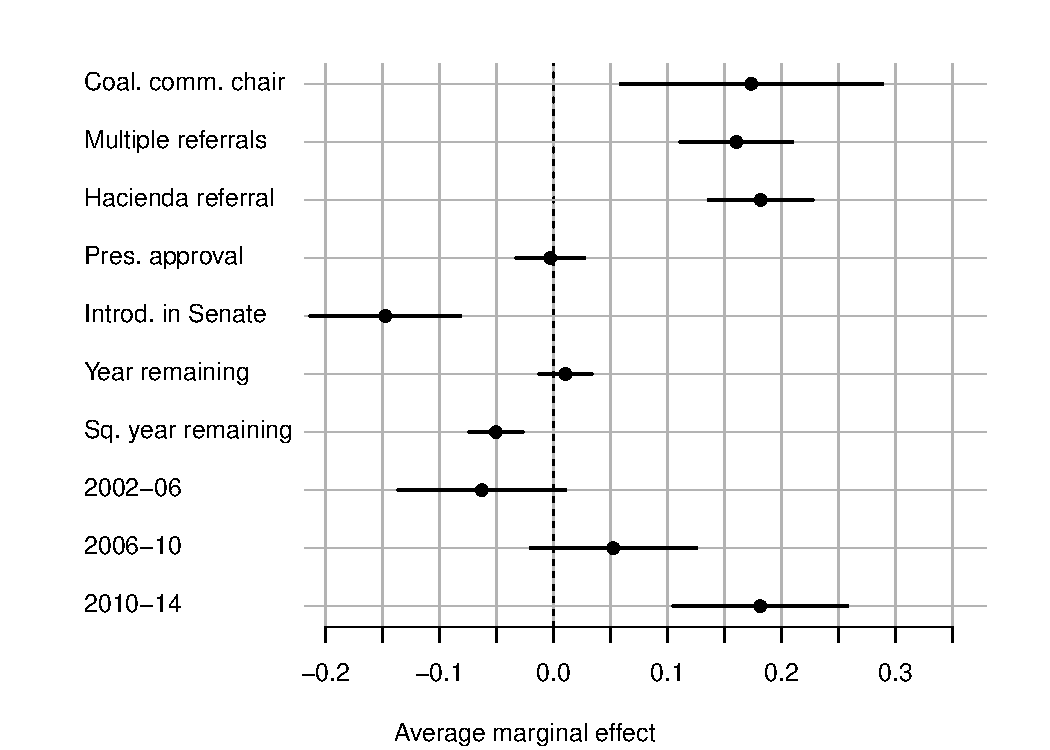
\includegraphics[width=.8\columnwidth]{../graphs/avgMgEffects.pdf}
\end{figure}

Figure \ref{F:avgMg} reports changes in the average predicted probability that a bill is fast-tracked associated with unit changes in model 3's explanatory variables (all other regressors at their mean value). This is a convenient way to gauge logit regression coefficients, by translating them into interpretable quantities. The report from a committee with a coalition chair experiences a 0.17 hike (0.06 standard error) in the likelihood of receiving a closed rule compared to a report by an opposition-chaired committee. The effect is as big as the average marginal effects of \emph{Hacienda Referral} (0.18), which capures mostly high-significance draft laws, and that of \emph{Multiple Referrals} (0.16), which we view as an indicator of issue complexity. We therefore find no statistical evidence to reject our Hypothesis 1. The results also confirm hypothesis 2, showing that a bill reported by a generally less friendly committe (chaired by the opposition), has a higher probability of receiving an open rule on the floor, thereby allowing the floor majority to bring back the bill to the median through floor amendments. Thus, presidents use open rules to control bills coming from preference distant committee chairs.

The substantial effects of \emph{Hacienda Referral} and \emph{Multiple Referrals} deserve comment. They suggest, first, that when spending gets in the way, restrictive rules are the norm in Chile. Recall that \emph{Multiple Referrals} exclude the Finance Committee, so there is an independent effect of bills with jurisdictional overlaps worth investigating further, and which must be associated, in part at least, to influencing the report through a friendlier committee.\footnote{We are grateful for this insight from an anonymous referee. According to \citet[][:118]{sotoCongChile2015}, multiple-referees may act sequentially or in tandem, as decided by the Cámara's presiding officer. When sequential, a divergent secondary committee's report is treated as an amendment to the primary committee's---an urgency overrides the secondary (an subsequent) report(s). We unfortunately lack information on this important aspect of multiple referrals.} Furthermore, note that the Finance Committee was always chaired by a coalition member but, with the exception of the 1998 to 2000 period, never by a co-partisan of the president. This may explain the milder effect of the partisan specification of our key variable in model 1. 

%Two alternative specifications ... With the exception of \emph{Senate Minority}, gaining in size and achieving .1-level significance, estimate changes are negligible. The change attests that the 2010--14 Legislature, with presidential minority status throughout (the 1998--2002 had short lapses only) experienced bigger inter-chamber differences in urgency incidence. The simpler urgency models are quite robust. 

%The strategic environment controls get mixed results. Neither coefficient for \emph{Pres.~Approval} nor \emph{Senate minority} achieved statistical significance. But \emph{Introduced in Senate} did. Bills successfully passing the upper chamber before moving to the Cámara were likelier to get urgent status, and the effect is significant at the .006 level. Proposals initiated in the Senate, where the opposition was systematically larger (and at times controlled the chamber) were, other things constant, also likelier urgency targets. Note also this coefficient's sizable hike from model 1 to model 2, gaining about a third in size while other coefficients did not change when controls for member-bill sponsorship are added. The lower initiation of mix-member bills in the Senate, as opposed to the Cámara (a $-.34$ correlation between \emph{Introduced in Senate} and \emph{Member bill, mix-sponsored}) masks a portion of the effect when sponsorship controls are omitted. 

%Both time trend variables returned significant coefficients. Other things constant, bills were likelier to become urgent earlier in the term and earlier in the legislative year. The apparent contradiction of the patterns in Figure \ref{f:depvarHistog} is explained by the distinction of non-original urgency messages---where most of the temporal trend is manifest---which is disregarded by the dichotomous measure of urgency analyzed here. 

Another effect worth highlighting is \emph{Introd.\ in Senate}. Bills successfully passing the Upper Chamber first, where the opposition was systematically larger and at times in control, were much less likely to get urgent status (the average marginal effect is $-0.15$ and significant). This suggests that agreements and compromises reached in the Senate ignited less, not more, protection from floor amendments in the \emph{Cámara's} plenary, most likely as a consequence of the greater preference divergence between the President and the opposition-led Senate. Analysis of inter-chamber negotiation and the reliance on urgency in the Upper Chamber are interesting venues for future research. 

\begin{figure}
  \centering
    \caption{Probability of fast-track bill consideration. Predictions are from from model 3 letting \emph{Year Remaining} vary in full range, with 95-percent confidence bands. Other variables set at the following values: $\text{\emph{Multiple Referrals}}=0$, $\text{\emph{Hacienda Referral}}=0$, $\text{\emph{Introd.~in~Senate}}=0$, $\text{\emph{2006-10}}=1$, and $\text{\emph{Pres.~Approval}}=.33$ (Bachelet's mean).}\label{F:sims}
    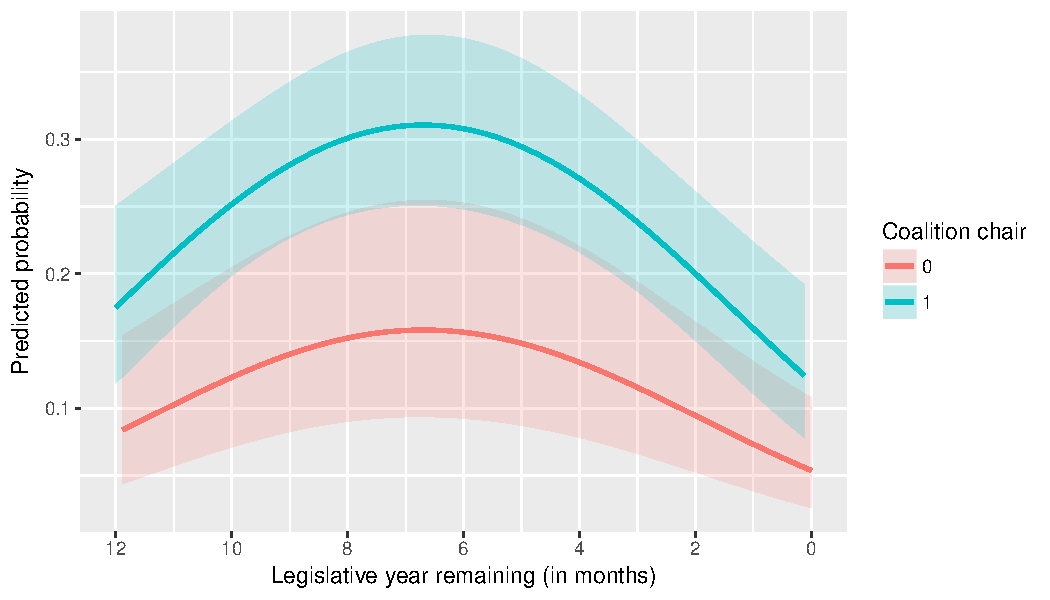
\includegraphics[width=.75\columnwidth]{../graphs/predictedPr.pdf}
\end{figure}

Finally, there are time trends in fast-track authority that simulations reveal neatly. Figure \ref{F:sims} portrays the predicted probability that a bill enters the fast-track throughout the legislative year. Regressors in model 3 are held constant to simulate a bill sent to the \emph{Cámara} in the 2006--10 Legislature that was referred to a single committee, excluding \emph{Hacienda}. \emph{Presidential Approval} (insignificant across models) is set to the mean for President Bachelet's first term, coinciding in full with the 2006--10 Legislature. The inverted-U shape shows how fast-track probability, predicted at 0.17 for coalition-chaired committees at the start, and 0.08 for the rest, becomes much likelier in the first half of the legislative year. By the second quarter (June--August), the probability is at its peak, about 0.32 percent and 0.17, respectively. It then experiences a sharp drop, ending the austral Summer break at 0.13 for coalition-chaired committees, and 0.05 for others. And while 95-percent confidence bands overlap, they barely do so at the middle of the legislative year, lending confidence that we are picking up a signal and not just random noise. 

\section{Discussion}\label{s:discussion}

This paper has argued that beyond the effect of urgency authority on the timing and deadlines for bill consideration, its procedural effects conceal a much more significant effect, by allowing presidents to shield desired policy from amendments on the floor. Furthermore, the president's decision not to use this tool is also important. An open rule means that bills can receive amendments on the floor that may move it closer to the president's preferences. This paper portrays urgency authority, found in seven Latin American constitutions, as equivalent to the fast-track authority that United States presidents enjoy periodically. Doing so shows how proposals that presidents qualify as urgent are considered under restrictive rules by the chamber's plenary: they must be voted up-or-down, without amendments.

While all seven constitutions remain silent about the procedural implications of urgency authority, and we have only looked for these restrictive procedures in statutes and chamber rules in the case of Chile, there are good reasons to expect that other countries have included similar provisions. After all, the rationale of the urgency authority is expediting the legislative process, and restrictive rules are a natural choice to speed urgent bills' consideration before an explicit deadline expires. 

The classification of constitutional urgency authority into the plenary arrest (Brazil), automatic adoption (Ecuador, Paraguay, Uruguay), and indeterminate (Chile, Colombia, Mexico) variants, which we presented in Section 2, naturally brings two pending issues to the fore. One is cross-national validation of the presence of restrictive procedures at the level of statutes or chamber rules---especially where urgency effects are seemingly indeterminate, as in Chile. The task ahead is to identify procedures that restrict the choices available to legislators, such as closed rules do in Chile. The other is the need to model the bargaining logic of plenary-arrest and automatic-adoption variants in search of similarities and differences with the urgency-as-fast-track. We expect these efforts to generalize our argument beyond Chile, our case study. %this is key and very transparent in establishing the scope.

Game-theoretic treatment of urgency-as-fast-track authority shows that preference overlap between the president and the reporting committee is the mechanism driving the choice to put bills on the fast-track. The reverse also applies: bills referred to opposition-chaired committees, who might report them to the floor with fundamental changes, are less likely to be fast tracked. The president would prefer them to go to the floor with an open rule, especially if on the floor a (friendlier) majority can restore the original intent of the president and her party. Systematic analysis of proposals in the Chilean lower chamber in recent years yields evidence that, other things constant, bills reported by committees chaired by members of the president's coalition/party are about twice as likely to be fast-tracked than the rest. To the extent that parties and coalitions indicate preference overlap (as is accepted in Chile), the evidence supports our main theoretical result.

The paper's results and findings are of natural interest to students of comparative political institutions, especially those interested in legislative procedure and separation of powers. They also shed light on the field of American Politics. In a provocative book, \citet{howell.moe.Relic2016} make an argument in favor of giving U.S.\ presidents permanent fast-track authority not limited to trade agreements. In order to have a coherent and effective government, they argue in favor of constitutional reform to put the executive at the center of the legislative process: ``presidents should be granted enhanced agenda-setting powers to propose bills to Congress, which Congress should then be required to vote on without amendment, on a strictly majoritarian basis, within a fixed period of time'' (145). Failure to vote in due time would turn those bills into law. Equating urgency and fast-track authorities shows this to be the automatic adoption variant. Reform would therefore make U.S.\ presidents similar to those in Ecuador, Paraguay, and Uruguay in this respect. 

Our results also speak to students of executive decrees and unilateral policymaking more generally. As discussed in the introduction, urgency authority and decree authority may overlap, as in fact they do in Brazil, Chile, and Colombia. We have established that, while urgency authority increases the president's leverage over the legislative process, an agreement is needed between the president and her congressional allies without which this prerogative is rendered powerless. Congress retains authority to reject urgent proposals, and cannot therefore be made worse-off than the status quo. Executive decrees, on the other hand, imply an abdication of decision rights on the part of legislators to participate in the process, and force legislators to respond to the president's enacted decree instead once it has already altered the status quo.

Yet for this precise reason executive decrees are not a true alternative in certain cases \citep{palanza.2019}. \citet[][:164]{figueiredo.limongi.2000} report that urgent bills in Brazil are quite rare since the provisional decree ``is a much more efficient way of speeding up and approving legislation.'' and more research should be done to establish whether effectively the urgency prerogative is used, for instance, on issues that are excluded from executive decree authority in the Brazilian constitution. Previous findings indicate that reliance on decrees effectively diminishes when policy deals with these issues --although it does not disappear. It is undeniable that Chile, where executive decrees are seldom used (only two decrees have been enacted since 1990), resorts to urgency authority expansively. Future research, and hopefully comparative work, will help tackle this issue. 

Chilean legislative scholars will find interest in investigating a missing piece in our argument. To be clear, the research advanced in this paper sheds light on the factors that affect the likelihood of reliance on urgency authority, and we provide an argument explaining the mechanism that leads to this usage. But we do not provide verification that closed rules do in fact dispel amendments---a key and untested premise of our approach. Systematic contrasting of bills that presidents drafted in the period, the various amendments that were introduced, the committee reports, and the text ultimately adopted, would enable analysts to demonstrate whether or not urgencies in fact dodge amendments. This is a difficult but promising venue for future research. 

Last, we emphasize that our investigation contributes to the literature on restrictive procedures. To the general class of procedures as instruments of political control, we add the urgency authority. One difference sets fast-track mechanisms apart from standard closed rules. Standard restrictive rules give agenda power to legislators---it may be the plenary \citep{mcnollgast.1987}, standing committees \citep{weingast.1992}, the bicameral conference \citep{shepsle.weingast.1987}, or the majority party \citep{cox.mccubbins.1997}. Urgency puts the executive in control of protecting vulnerable legislative agreements. The unique role and function to determine whether or not a major bill will be considered in the U.S. House, and which amendments and motions will be allowed, is firmly in control of the legislative leadership, acting as sole gatekeepers to the plenary \citep{cox.2006}. As with France's \emph{vote bloqué} \citep{huber.1996b}, fast-track authority lets the executive branch pull some of the gatekeeping levers, earning a priceless legislative prerogative worthy of further research.

\section*{Author contributions}

We describe contributions to the paper using a standard taxonomy \citep{allen2014credit}. E.\ Magar (EM) was lead author, having taken primary responsibility for methodology, computation, formal analysis, and data collection and curation. G.\ Sin (GS) was responsible for comparative constitutional research. V.\ Palanza (VP) was in charge of funding acquisition. EM prepared the original draft and revision for resubmission. VP lead text editing and review, with contributions from GS. All authors contributed equally to conceptualization and article framing. 

%% McCox 2nd Ed leviathan, fn 5 p. 214: ``Congressional Quarterly (1994 <-- 19nov, 3326) describes the role played by the modern Rules committee: The Rules committee is the gatekeeper to the House floor. It has a unique role and function, determining how and whether a major bill will be considered on the floor, and which amendments and motions will be allowed. This gives the committee considerable power in shaping the legislative agenda and makes it the arbiter of frequent turf fights between other committees.''  

%Yet inspection of recent urgency message incidence reveals a strikingly high frequency: one of every five bills in Congress received some form of executive urgency at some stage (and often at several stages) of the legislative process; and more than two-thirds of executive proposals did. Adding a layer to the puzzle, Congress in fact complied with a significant number of urgency messages. Why would presidents resort so remarkably frequently to the institutionally inconsequential urgency authority? And why would legislators comply so often with empty executive threats?



%% TODO ESTO VIENE DE ANTERIOR VERSION... DESCOMENTAR PARA VER QUE ES RESCATABLE

%% \section{The received wisdom}

%% \begin{center}
%% \singlespacing
%% [U]rgency powers... can have dramatic effects on executive-legislative \\ 
%% relations, legislative organization, and the policy process more generally\\ 
%% ---\citet[][:438]{morgenstern.2002b}
%% \end{center}
%% \onehalfspacing

%% %\citeauthor{carey.shugart.1998a}'s \citeyearpar{carey.shugart.1998a} monograph on executive unilateral powers does not discuss it. \citeauthor{londregan.2000a}'s \citeyearpar{londregan.2000a} study of legislative institutions in the Chilean Senate does not include urgency authority in the index. 

%% \noindent Scholars have paid little attention to urgency authority. \citeauthor{shugart.carey.1992}'s \citeyearpar{shugart.carey.1992} seminal monograph does not include it when computing the index of presidents' legislative powers. And while not addressing it directly either, \citeauthor{carey.shugart.1998a}'s \citeyearpar{carey.shugart.1998a} discussion of the delegation of unilateral authority to the executive offers clues of the logic behind the institution. Informational and valence asymmetries between Latin American executive and legislative branches create incentives for such delegation. Delays to reach agreement in assemblies offer further incentives by diminishing the value of policy \citep{baron.ferejohn.1989}, so rather than delegate proposal power within the chamber, legislators may find it preferable to let the president set the agenda. 

%% %\citet{siavelis.2002} is the first study to cover urgency authority. He hypothesized urgencies' game-changer potential. His study of Chilean executive-legislative covers the first post-transition presidency revealed just how very frequently urgency messages were issued: slightly more than one-third of proposals in Congress received some form of urgency, and about 9 out of 10 of urgent bills were executive-initiated. Guided by semantics, analysis sought to discover if urgent bills, in fact, circulated the steps of the legislative process faster than the rest, and whether urgency status also increased the likelihood of bill passage. The study found mixed evidence. Among executive bills, consideration of urgent ones had somewhat shorter duration than the rest (medians of 134 and 160 days, respectively), but no palpable difference in success rates is appreciated (64 and 63 percent, respectively). 

%% \citet{siavelis.2002} is the only systematic study of urgency authority we are aware of. Like Morgenstern's quote, he hypothesized urgency power's game-changer potential. His study of Chilean executive-legislative in the first post-transition administration revealed the amazing frequency with which urgency messages were issued by President Aylwin: slightly more than one-third of proposals in Congress received some form of urgency, and about 9 out of 10 of urgent bills were executive-initiated. Guided by semantics, he also sought to discover if ``urgent'' bills, in fact, circulated the steps of the legislative process faster than the rest, and whether urgency status increased the likelihood of bill passage. The study found mixed evidence at best. Among executive bills, consideration of those urgent had somewhat shorter duration than the rest (medians of 134 and 160 days, respectively), but no palpable difference in success rates is appreciated (64 and 63 percent, respectively). 

%% The negative finding may bear relation to three elements. In their study of budgetary congressional oversight of the executive, \citet{berrios.gamboa.fiscChile.2006} warn against overstating the Chilean urgency authority's importance, as non-compliance entails no penalty for Congress---the next section develops this argument. While this may explain the lack of effects, it begs the question of why the president resorted so frequently to an authority that seems inconsequential. In other words, why make so many empty threats?

%% Another is a failure to control for urgency degrees---elaborated in section 3---in the analysis. \citeauthor{aleman.navia.UrgChi.2009}'s \citeyearpar{aleman.navia.UrgChi.2009} systematic study of executive success in Congress in three post-transition presidencies finds some of the evidence sought by Siavelis. Controlling for bill characteristics (such as key policy domains, the chamber where the bill originated, the government's seat margin, and presidential agenda size), urgency degrees had quite different effects in passage. Higher degrees significantly associate with better probability of executive success, but the lower made no statistical difference. Since, as will be seen, low-degree urgencies were much more prevalent, conflating them washes off the effect of the higher-degree. 

%% % longer review of aleman and navia
%% %\citeauthor{aleman.navia.UrgChi.2009}'s \citeyearpar{aleman.navia.UrgChi.2009} systematic study of executive success in Congress in three post-transition presidencies also inspects Chile's urgency authority. Among controls, their equation includes urgency authority usage in the right side. The unit is the individual bill, and the size of the executive agenda varies substantially over the years. Variation is quantitative  (Congress received about 150 presidential bills in each of the first 6 years after 1990, a numbrer that dropped to about 70 in the next 6 years, then climbed to about 100 in the final 4 years of their series) and qualitative, presidents manifesting different propensities to aim at constitutional reform. Of direct relevance are the findings on urgencies. Controlling for key policy domains, chamber of origin, seat margins, and presidential approval, and clustering errors by legislative year, different prioritization reveal quite different effects in passage. `Act now' and `2-week' notices significantly increased the probability of bill passage, but not `one month' notices. 

%% Finally, selection bias is an obstacle to measure urgency authority effects. Presidents, behaving strategically, are likely to target for urgency proposals that are markedly different from the rest in important ways, so the set of bills receiveing urgent status is not random. Like the Siavelis and Alemán-Navia studies, we recognize the endogeneity problem that arises but does not confront it methodologically. Until a more subtle identification design is proposed, findings must be taken with a grain of salt. The systematic study of urgency authority in Chile that follows should contribute to pave the way to a solution. 

%% %If presidents, behaving strategically, were to target for urgency proposals that are markedly different from the rest in important ways, a problem of endogeneity arises. Classify proposals based on how difficult passage is expected: easy, hard, and impossible. If left on their own, the easy proposals would be approved faster, the hard slower, the impossible never. A strategic president should concentrate urgency authority in the hard group, leaving easy proposals mostly on their own, while abandoning the hopeless group of impossible proposals, that will not be observed. As a consequence, comparing

%% %The relevant quantity of interest is whether the use of urgency authority affects bill passage (success, speed, amendments, and so forth) compared to the same bill with no urgency attached. The fundamental problem of causal inference is immediately evident. The executive presumably targets bills for urgency strategically, so that the selection mechanism cannot be assumed random. If, for example, more complex and divisive legislation takes longer, is likelier to fail and likelier to be tagged urgent, separating effects requires more subtle methods than used up to now.


%% \section{Variable urgency degrees}
%% \begin{center}
%% Presidential power is the power to persuade ---Neustadt\footnote{\citet[][:11]{neustadt.1990}}
%% \end{center}


%% Vagueness surrounds key aspects of urgency authority. When a 30-day limit is set, for instance, no indication is given of whether those are calendar, business, or session days. I treat the messages in weeks rather than days given imprecision (and, when coding deadlines in the empirical sections below, rely on business days, as \citet[][:285]{sotoCongChile2015} suggests). More important, no formal reversionary course of action is defined, and no hint of rulings by the Constitutional Tribunal filling in the institutional void could be found. As seen in the previous section, I interpret indeterminacy as reversion to the status quo with no effect on the voting schedule.


%% %Urgency type frequency, in fact, reveals a tendency to rely less often on more urgent messages (descriptive data is presented in the next section). `Act now' notices were roughly 3 to 5 times less frequent than `two week' ones in a recent 16-year period. The frequency differential between `two week' and `one month' notices is less sharp, but a tendency is distinguishable. 


%% \section{The data}


%% % \begin{table}
%% % \begin{center}
%% % \begin{tabular}{rrr}
%% % Number of &      Bill &     \\
%% % messages  & frequency &  ~~~~~~~~\% \\ \hline
%% % %None              &  5635     &     \\
%% % 1                 &  214      &  \emph{16}   \\
%% % 2                 &  242      &  \emph{18}   \\
%% % 3                 &  145      &  \emph{11}   \\
%% % 4                 &  115      &  \emph{8}    \\
%% % 5                 &  104      &  \emph{8}    \\
%% % 6-10              &  236      &  \emph{17}   \\
%% % 11-20             &  183      &  \emph{13}   \\
%% % 21-40             &  99       &  \emph{7}    \\
%% % 41-71             &  24       &  \emph{2}    \\
%% % Total             & 1,362     & \emph{100}   \\ \hline
%% % \end{tabular}
%% % \caption{Urgent bills classified by number of urgency messages received}\label{T:billFreqByNurg}
%% % \end{center}
%% % \end{table}

%% % Other interesting patterns in urgency authority usage are discernible in bill histories. Assessing how large the subset of bills receiving one or more urgency messages is conveys a minimalist perspective of urgency authority. As shown in table \ref{T:billFreqByNurg}, most bills in this subset (84 percent) in fact received many such messages, and a substantial portion (40 percent) received between 6 and 71 urgency messages. This raises another puzzle for research. Are presidents reiterating urgency messages because of Congressional inaction? Extending the deadline may help the president save face when legislative non-compliance is imminent. Or are presidents micro-managing select-bill consideration in committee, monitoring a report's progress and then sending recommendations in the message extending the deadline? The source indicates the arrival of presidential messages but does not include their actual contents, nor those of committee reports. Archival research to retrieve those documents would do wonders in answering these questions. 

%% %A bicameral process operating on a single-round navette \citep{tsebelis.money.1997}---bills migrate from originating to revising chamber, back to originating if amended, and finally to conference if inter-cameral differences persist---offers, at most, four clear instances for repeated urgency authority use. Yet, as table \ref{T:billFreqByNurg} reports, nearly half of urgent bills (47 percent) received five messages or more. A handful of bills received several dozen messages! 

%% \begin{figure}
%% \begin{center}
%%  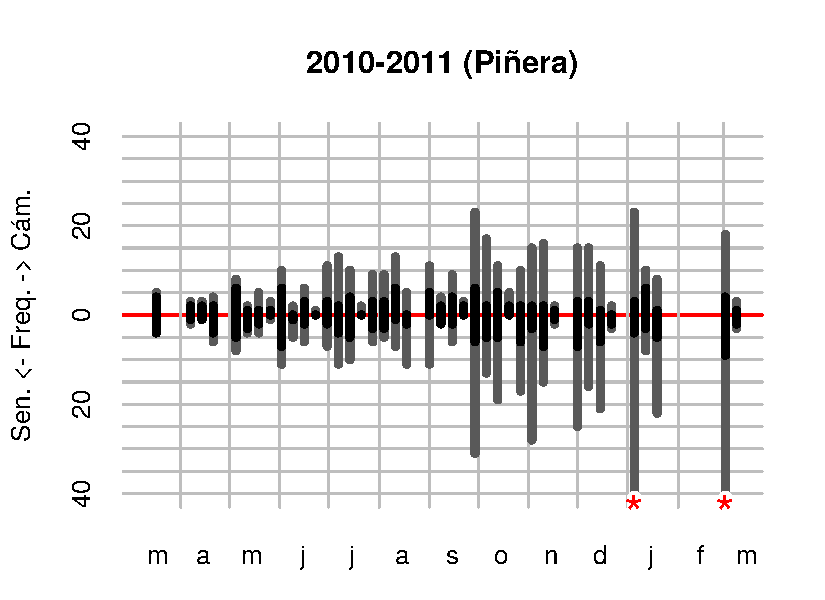
\includegraphics[width=.65\columnwidth]{../graphs/urgenciasHistog2010.pdf}
%% \begin{tabular}{cccc}
%%     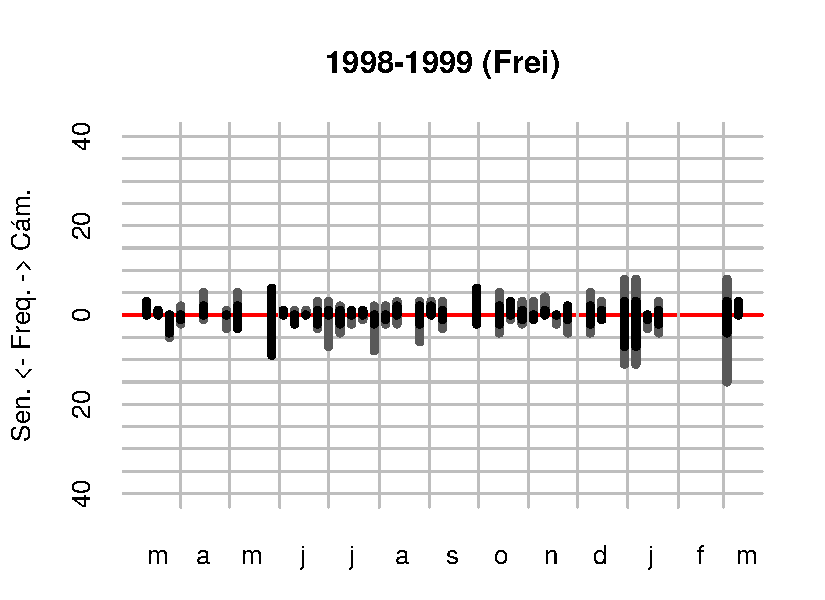
\includegraphics[width=.22\columnwidth]{../graphs/urgenciasHistog1998.pdf} &
%%     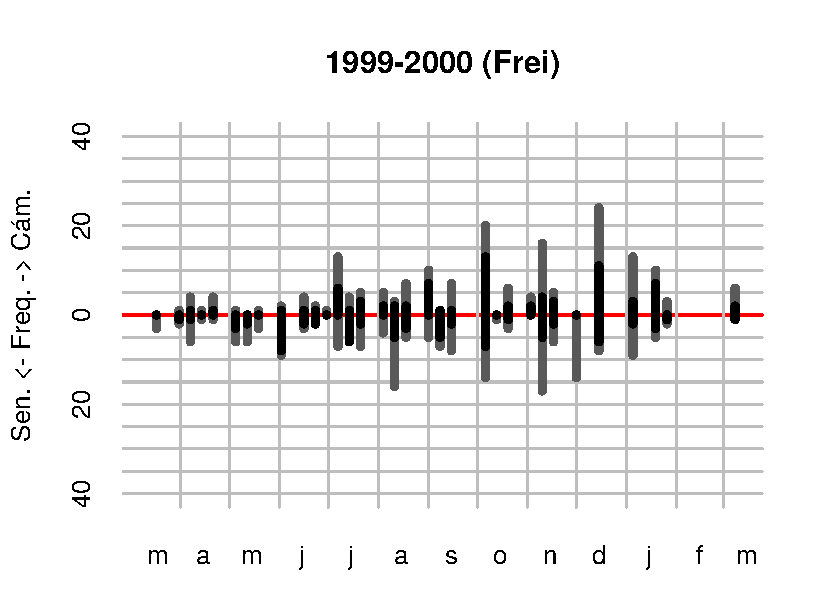
\includegraphics[width=.22\columnwidth]{../graphs/urgenciasHistog1999.pdf} &
%%     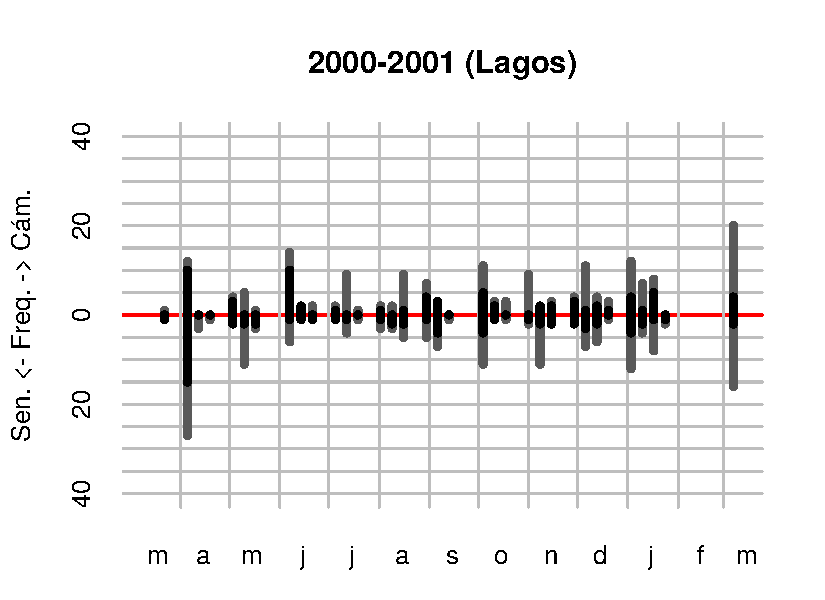
\includegraphics[width=.22\columnwidth]{../graphs/urgenciasHistog2000.pdf} &
%%     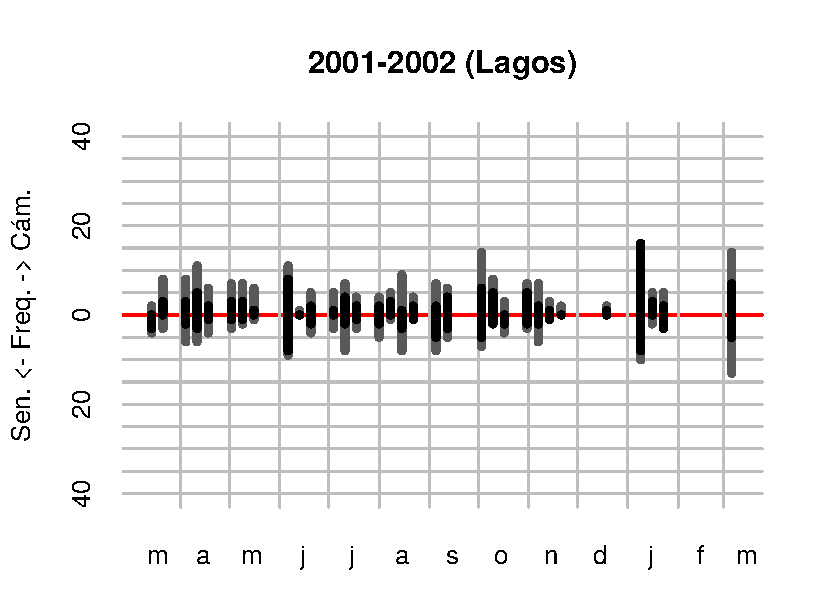
\includegraphics[width=.22\columnwidth]{../graphs/urgenciasHistog2001.pdf} \\
%%     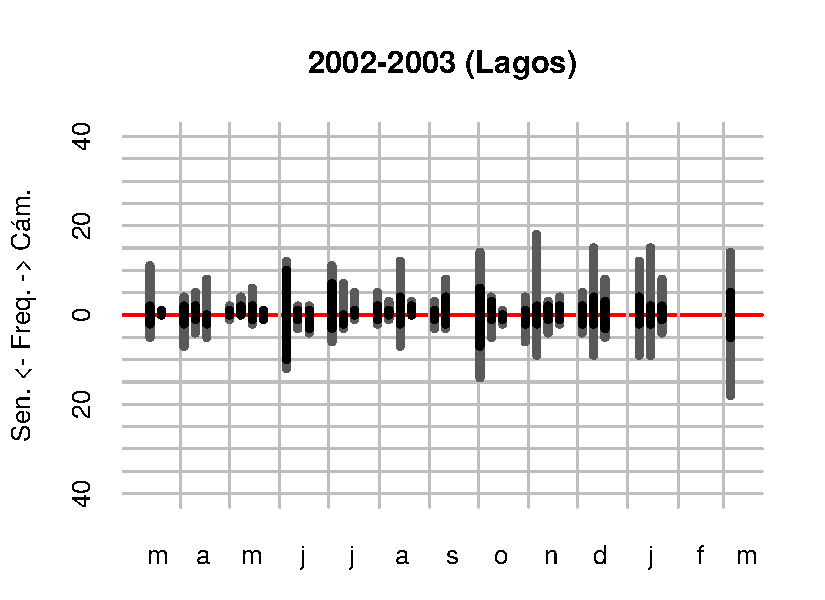
\includegraphics[width=.22\columnwidth]{../graphs/urgenciasHistog2002.pdf} &
%%     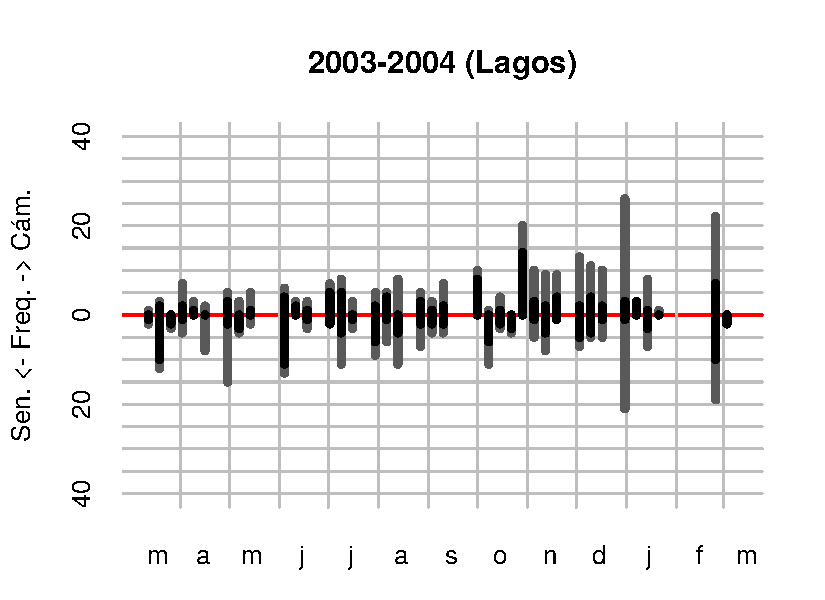
\includegraphics[width=.22\columnwidth]{../graphs/urgenciasHistog2003.pdf} &
%%     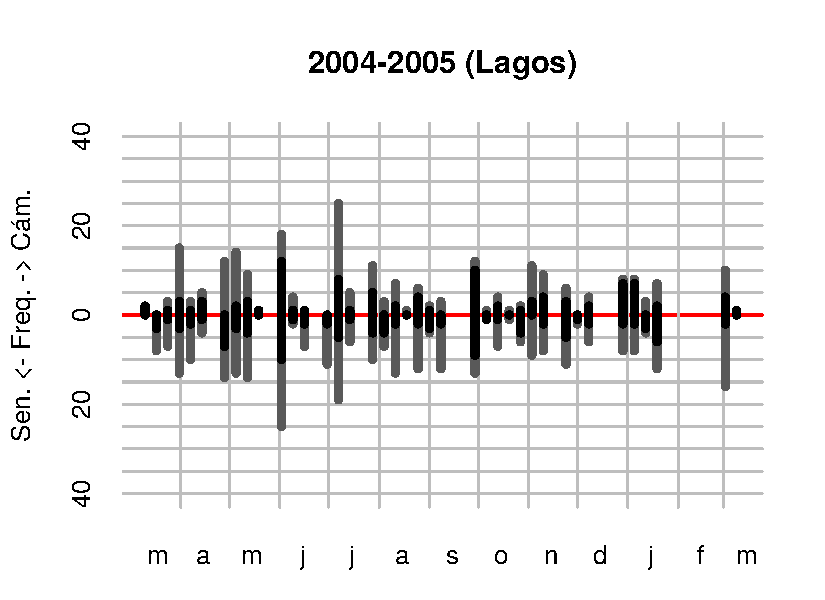
\includegraphics[width=.22\columnwidth]{../graphs/urgenciasHistog2004.pdf} &
%%     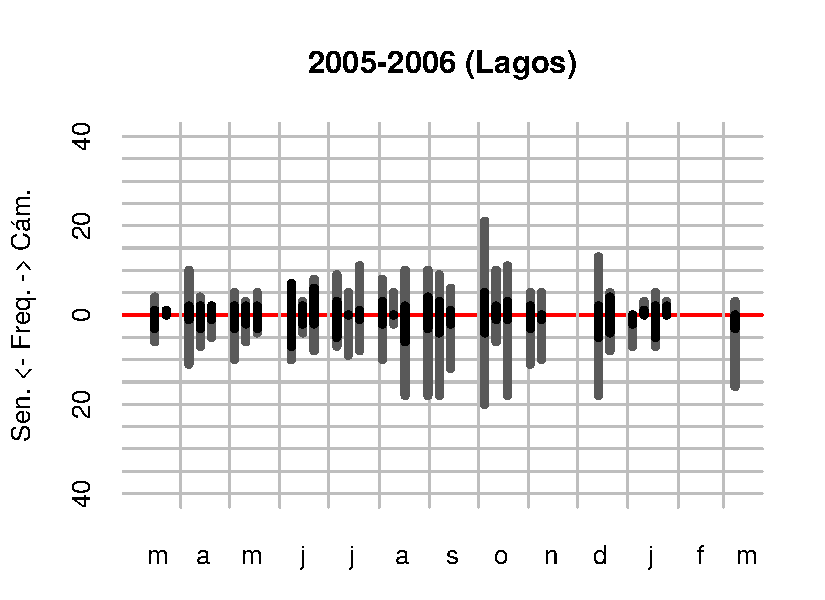
\includegraphics[width=.22\columnwidth]{../graphs/urgenciasHistog2005.pdf} \\
%%     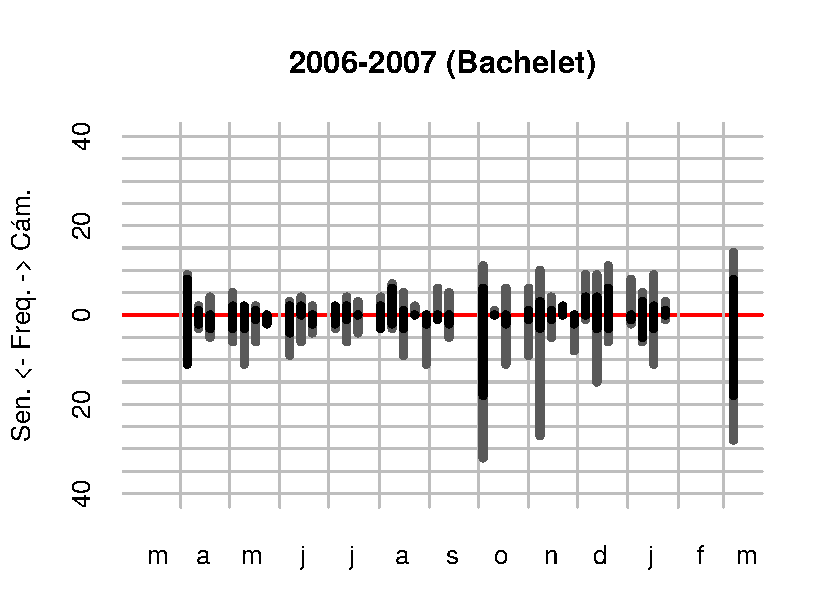
\includegraphics[width=.22\columnwidth]{../graphs/urgenciasHistog2006.pdf} &
%%     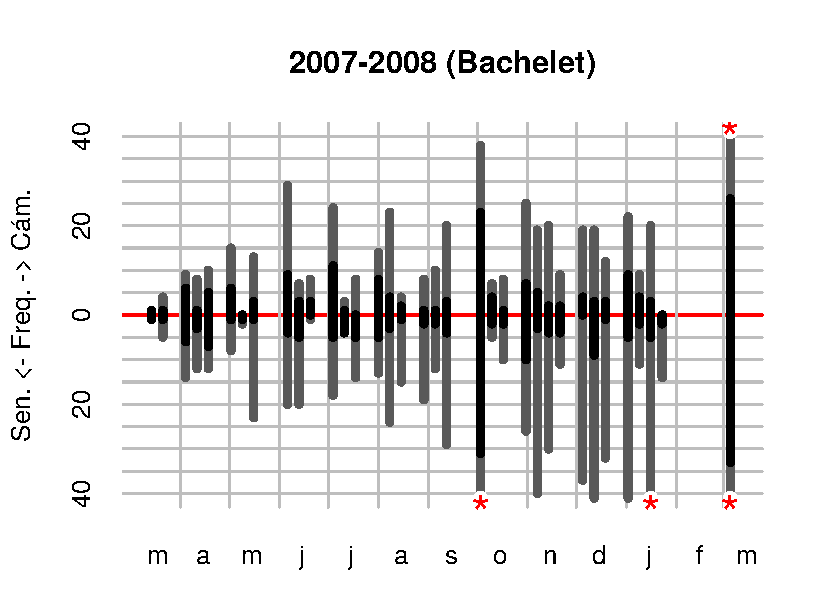
\includegraphics[width=.22\columnwidth]{../graphs/urgenciasHistog2007.pdf} &
%%     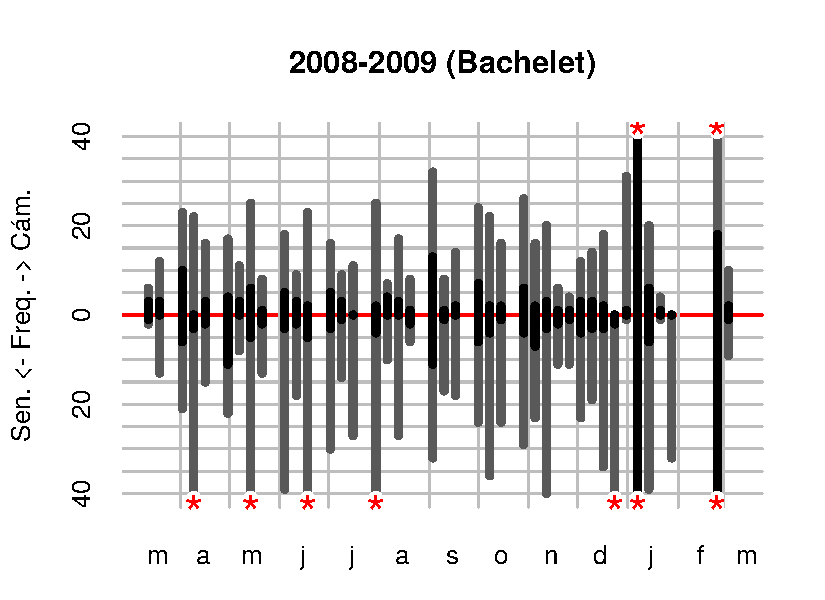
\includegraphics[width=.22\columnwidth]{../graphs/urgenciasHistog2008.pdf} &
%%     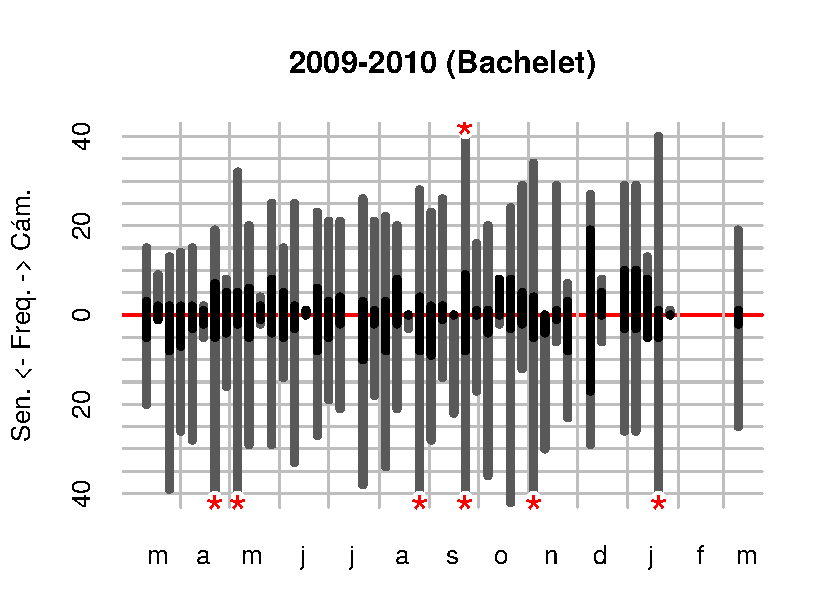
\includegraphics[width=.22\columnwidth]{../graphs/urgenciasHistog2009.pdf} \\
%%     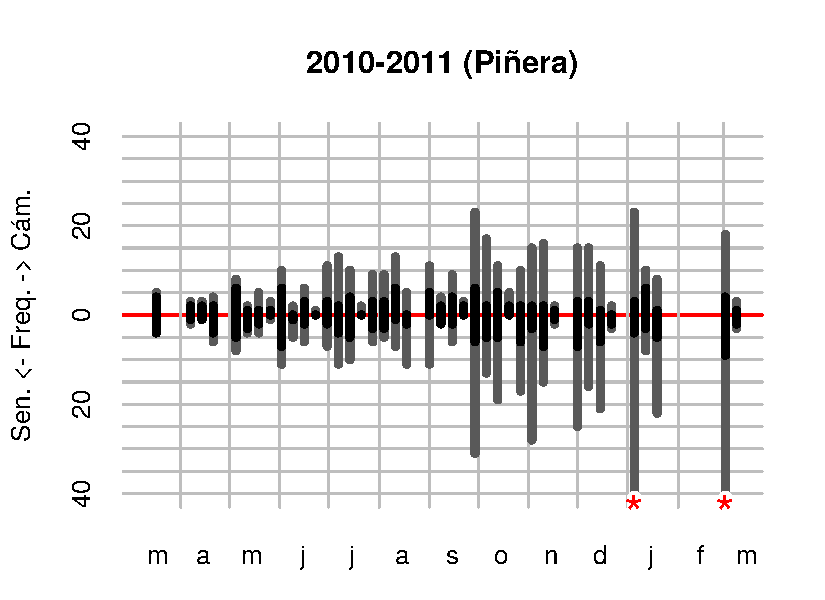
\includegraphics[width=.22\columnwidth]{../graphs/urgenciasHistog2010.pdf} &
%%     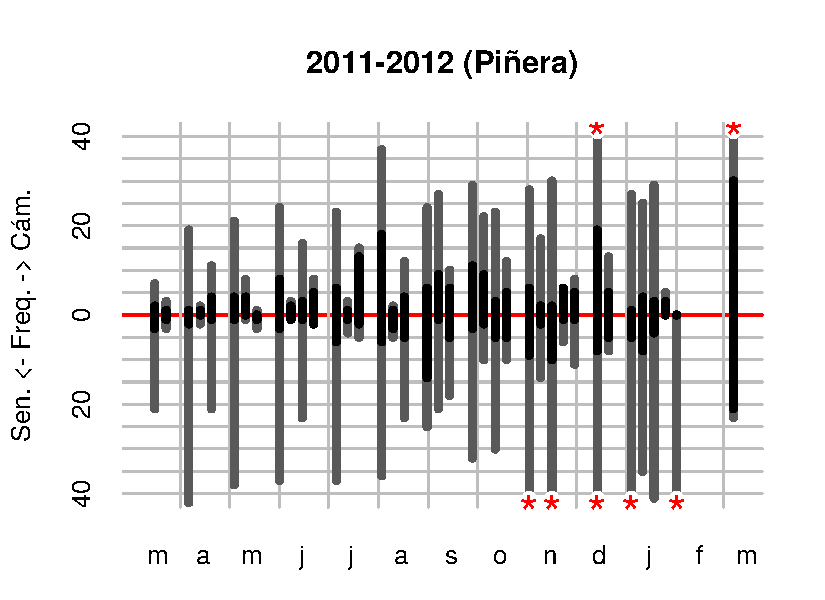
\includegraphics[width=.22\columnwidth]{../graphs/urgenciasHistog2011.pdf} &
%%     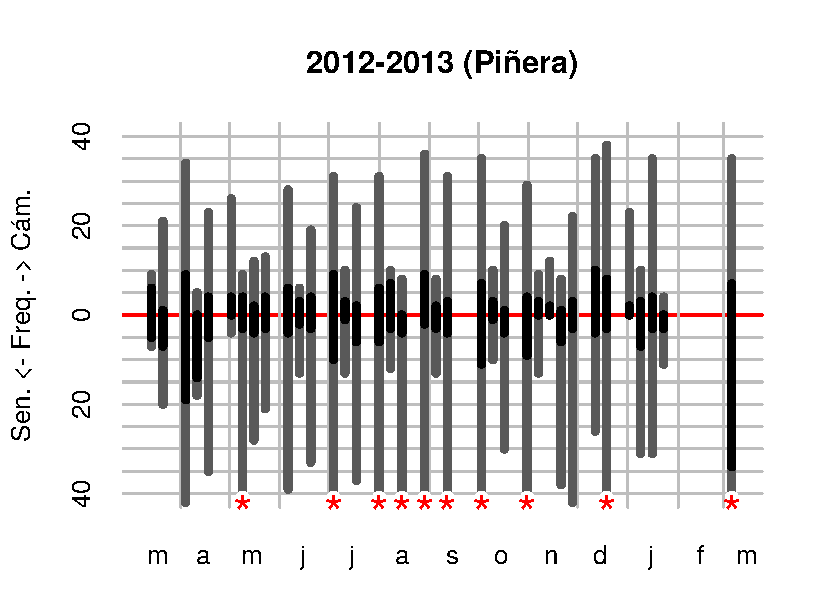
\includegraphics[width=.22\columnwidth]{../graphs/urgenciasHistog2012.pdf} &
%%     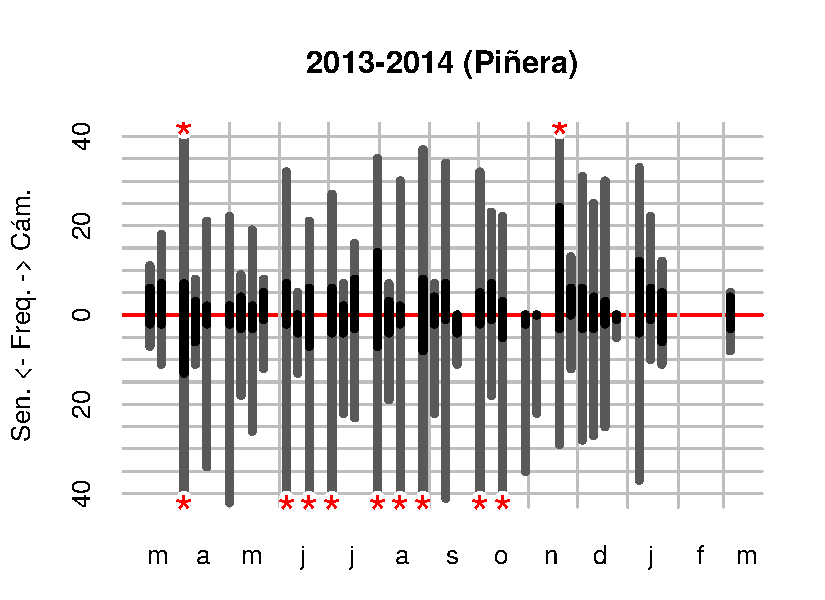
\includegraphics[width=.22\columnwidth]{../graphs/urgenciasHistog2013.pdf} \\
%% \end{tabular}
%%   \caption{Weekly urgency messages by legislative year. Cámara histogram above, Senate below the zero line. Black portion of bars indicates original urgencies, gray portion indicate deadline changes and urgency withdrawals. Asterisk atop column indicates off-the-chart urgency message frequency.}\label{f:depvarHistog}
%% \end{center}
%% \end{figure}

%% % \begin{figure}
%% % \begin{center}
%% %     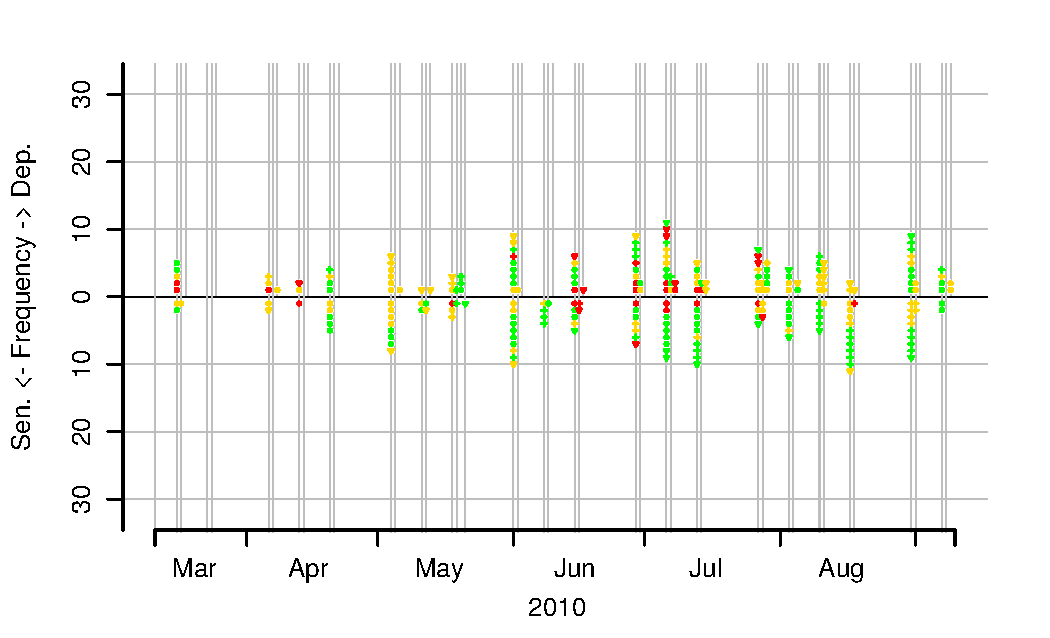
\includegraphics[width=\columnwidth]{../graphs/urgencias2010-1.pdf} \\
%% %     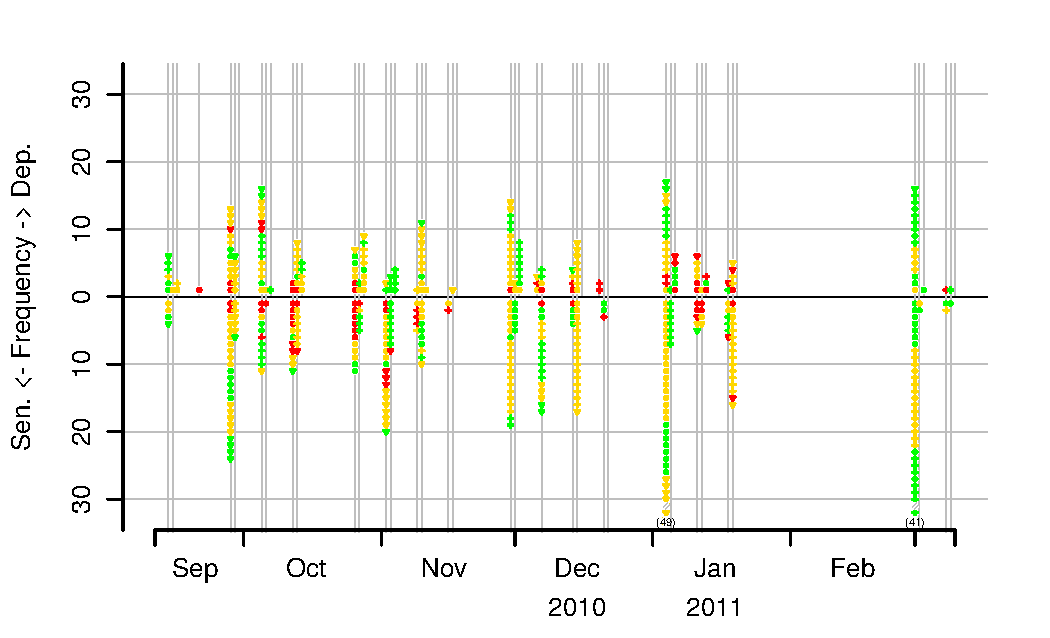
\includegraphics[width=\columnwidth]{../graphs/urgencias2010-2.pdf} 
%% %   \caption{Urgency messages in legislative year 2010--11. Diputados and Senate data above and below the zero line, respectively. Vertical gray lines indicate that a session took place. One point for each urgency message, a circle for a newly declared urgent bill, a plus sign for an urgent bill with new deadline, a triangle for an urgency withdrawn. Point color indicates urgency type, red for `act now', yellow for `two week', green for `one month'. Parentheses atop columns indicate off-the-chart urgency message frequency.}\label{f:depvar}
%% % \end{center}
%% % \end{figure}

%% Chains offer a better perspective of the evolution of urgency usage than sheer messages. The 170 percent message surge between the 2002--06 and 2006--10 Legislatures was, in fact, due to declaring 90 percent more legislation urgent, the rest attributable to substantially longer chains (4.2 links on average, up from 3). The 2010--14 hike is mostly due to longer chains (4.7 links on average), as the chain frequency increase was negligible. Plotting weekly urgency messages in the period, as Figure \ref{f:depvarHistog} does, reveals how original urgency incidence changed little over the years, unlike non-original message incidence. Each panel in the figure (one of which is zoomed above to provide detail) reports one legislative year as two super-imposed histograms, one for Cámara and one for Senate messages (both positive scales, red asterisks marking off-the-chart counts). The black portion of columns count original urgency messages, the gray count deadline changes and withdrawals. Note how black central segments had some tendency to grow in both chambers from year to year. But that change looks minute compared to how the gray fringes expanded. Urgency-wise, Presidents Bachelet (2006--10) and Piñera (2010--14) had relatively quiet first years in office, using the authority much more often after the second, and especially after the third year. Piñera's more insistent messages to the Senate than the Cámara, as seen in the red star asymmetry, coincided with a lack of majority in the chamber. 

%% \begin{table}
%% \begin{center}
%% %\begin{small}
%% \begin{tabular}{lrrrrrrrr}
%%                          &  \mc{8}{c}{Percent Concertación sponsors} \\
%% Urgency raised by        &  0\%      &  1--25    &  26--50    &  51--75    &  76--99    &  100\%      &  All         &  N \\ \hline
%% Concertación presidents& \emph{21} & \emph{3}  & \emph{10}  & \emph{15}  & \emph{13}  & \emph{39}   &  \emph{100}  &  228 \\
%% Right president          & \emph{26} & \emph{4}  & \emph{18}  & \emph{12}  & \emph{12}  & \emph{26}   &  \emph{100}  &  121 \\
%% \end{tabular}
%% \caption{Sponsorship of urgent member proposals. Entries are relative frequencies of Concertación sponsors among bills declared urgent by presidents elected by list given in row. The first entry reports that 21 percent of bills declared urgent by a Concertación president had not a single co-sponsor elected by that list; and so forth.}\label{T:sponsorsOfUrgBills}
%% %\end{small}
%% \end{center}
%% \end{table}

%% % ``Para evitar entorpecer el funcionamiento de Congreso, el Ejecutivo procura no tener, al mismo tiempo, más de 10 proyectos con urgencia en cada una de las Cámaras (entrevista Carmona)'' (fn.~25) Carmona citado en berrios gamboa

%% Also plain in figure \ref{f:depvarHistog} is the time scarcity problem. If urgency authority were consequential, the abundance of messages would pose a genuine scheduling problem for members and their legislative parties. Not taking the February Summer break into account (when Congress rarely convenes), the Cámara in the median legislative year had just 4 weeks free of original urgency messages, and none free of urgency messages of either type. Saturating the agenda with urgent executive bills inevitably plunders scheduling time to consider members' pet projects.\footnote{\citet{berrios.gamboa.fiscChile.2006} quote the executive's legal chief of staff describing a general goal in the Executive branch to have, at most, ten urgent projects in each chamber at once and thus ``prevent blundering congressional work (\emph{evitar entorpecer el funcionamiento de Congreso})'' (fn.~25). It is an optimistic assessment of presidential self-restraint, to say the least. If urgency authority were consequential, presidents who have taken the chamber's schedule hostage might be a better analogy than self-restraint.} The president may be taking the legislative schedule hostage \citep[cf.][]{cox.mccubbins.1994,williamson.1975}. In such circumstances, urgency authority is another asset for vote-buying, presidents freeing up scheduling time or even granting members' projects urgent status in exchange for support for difficult proposals. The evidencein table \ref{T:sponsorsOfUrgBills} is consistent with this conjecture: controlling for the percentage of signatures by legislators belonging to Concertación parties in the proposal reveals that presidents often granted urgent status to opposition bills. Of member bills declared urgent by Concertación presidents (1998--2010), 21 percent fell in this category, and 26 percent by the right-of-center administration that followed (2010--2014). This bonding perspective of scheduling is a promising line of research of executive-legislative negotiation. 

%% \section{Urgency chains}

%% Urgency authority predictors aide the interpretation of the next pieces of analysis. Units here are not individual bills but urgency instances, in search for correlates in the legislation they target. The previous section ignored urgency reiteration, a striking pattern in the data. This section isolates urgency chains in search for one observable consequences in the legislative process. If urgency authority were consequential, it should prompt action in the chamber where the bill awaited consideration. Moreover, the action should happen within the deadline established by the president. 

%% Several actions might follow an urgency call: the bill is marked in committee; one or more committee reports (called \emph{informes} in Chile) are drafted and adopted; the bill is reported, with possible revisions or even a negative advise, to the floor; a positively-reported bill is scheduled in the Order (\emph{Orden del Día}); the plenary considers, possibly amends, and eventually votes the bill's passage; and possibly others. Analysis here focuses on committee reports. Unlike some of the steps listed, reports are observable in the bill histories collected. If report contents are, unfortunately, unavailable in the data, the drafting committee(s) and report date(s) are included. Since urgency messages are also dated, synchronicity can be verified systematically.  

%% Committee reports are a good choice to search for urgency authority effects because only exceptional cases should not get one. Unless the floor votes an exception to the rules unanimously, every bill in Chile is referred to a standing or special committee upon first introduction to each chamber. Another exception are bills previously reported at the time the urgency call is made. A last exception are bills discharged from committee for direct floor consideration. No explicit discharge procedure could be found in the congressional standing orders, but presumably it is the same---unanimous consent---to consider a bill without prior committee referral. There is no record in the data to verify it, but the presumption is that such exceptions are rare. At any rate, exceptions play against detecting ripples caused by urgency authority.

%% One hypothesis of consequential urgency authority tested is that raising an urgency prompts a committee report. A finer hypothesis involves the chronology of events: if urgency authority were consequential, bill reporting should occur \emph{before} the given deadline expires. Because the terms of the urgency were modified so often in the period, chains---not individual messages---are considered for analysis, expecting reports on or before the chain's final deadline. Rejecting hypotheses weighs against consequential urgency authority, committees retaining the potential as formidable gatekeepers in their policy jurisdiction---failure to draft a report prevents the proposal from progressing in the legislative process \citep{cox.mccubbins.1993,fenno.1973,shepsle.weingast.1987}. 

%% %Due to the frequency with which deadlines are adjusted, expecting a timely reports for every message is unreasonable, even if the urgency authority were consequential. The relevant units are therefore not urgency messages but urgency chains: reports should antedate the final deadline set by a chain of messages. 

%% %This section analyzes bill histories to detect whether or not reports follow urgency messages in the Cámara de Diputados, and whether or not this occurs in a timely manner. Failure to observe the report is evidence of inconsequential urgency authority.  

%% As mentioned, the Hacienda committee has special status in the Chilean Congress and deserves attention. Unlike other committees, Hacienda has jurisdiction over \emph{every} bill authorizing spending in any domain. Moreover, the unanimous exception rule is inapplicable to Hacienda bills, which \emph{must} be reported to be considered in the floor.\footnote{Standing rules (Ley orgánica del Congreso) arts.\ 17 and 21.} So, for instance, a proposal restricting labor benefits to certain state health workers at the municipal level was referred to both the Public Health and Hacienda committees because a small appropriation for verification by the Labor Bureau was required. Hacienda committee members, working in tandem with Finance Ministry staff \citep{aleman.navia.UrgChi.2009}, may or may not appropriate funds from the budget in their report to the floor. Not unlike the Appropriations and Rules committees in the U.S.\ House, Hacienda has the status of a control committee, a key asset for agenda power \citep{kiewiet.mccubbins.1991}. Because Hacienda referral is mandatory, only previously reported bills would not get a Hacienda report following an urgency. 

%% The assessment of predictors of timely committee reports analyzes the subset of chains from bills that were referred to the Hacienda committee separately from the full set of chains in the period. The dependent variable equals 1 if a report (an Hacienda report in the chain subset) is observed on or before the deadline set by the final message in the chain (business days used for computation); equals 0 otherwise. The multivariate analysis includes predictors in the previous section (defined over chains instead of bills), minus Hacienda referral---a bill trait is controlled differently here---and presidential approval.\footnote{Including \emph{Pres.~approval} returns a statistically insignificant coefficient and produces negligible changes in other predictors.} Also in the right side are indicators for original urgency message types. \emph{2~week~notice} and \emph{1~month~notice} are mutually-exclusive dummies equal 1 if the first, or only, message in the chain is of the said type, respectively, and 0 otherwise. The omitted category are act now messages, which serve as baseline for coefficient interpretation. There are also indicators for reiterated messages. \emph{Change~deadline} equals 1 if at least one message extending or cutting short the original deadline is chained to the first urgency message; equals 0 otherwise. And \emph{Withdraw~urgency} equals 1 if the final message in a chain dropped the bill's urgent status; equals 0 otherwise. An alternative specification with 11 mutually-exclusive dummies (Act now singleton; Act now with deadline modified; Act now withdrawn; and so forth) yielded essentially identical results in a much less parsimonious equation.  

%% %The predictors used in the urgency models... \emph{Senate minority} and predictors listed below in Table \ref{t:chainsRegs}) are defined for chains instead of bills: Senate minority equals 1 if the opposition had majority status when the chain started and 0 otherwise; and so forth. 

%% % \begin{table}
%% % \begin{center}
%% % \begin{tabular}{lrr}
%% %                           &  \% chains      &              \\
%% %                           &  of type with   &              \\
%% %                           &  timely         &  (N Hacien-   \\ 
%% % Message type              &  Hacienda report&  da-referred)   \\ \hline
%% % Act now singleton         &               &  \\
%% % Act now, extend           &               &  \\
%% % Act now, withdraw         &               &  \\
%% % Act now, extend, withdraw &               &  \\
%% % 2 week singleton          &               &  \\
%% % 2 week, extend            &               &  \\
%% % 2 week, withdraw          &               &  \\
%% % 2 week, extend, withdraw  &               &  \\ 
%% % 1 month singleton         &               &  \\
%% % 1 month, extend           &               &  \\
%% % 1 month, withdraw         &               &  \\
%% % 1 month, extend, withdraw &               &  \\ 
%% % All                       &               &  \\
%% % \end{tabular}
%% % \caption{Urgency messages and committee reports within deadline}
%% % \end{center}
%% % \end{table}

%% % Table created by stargazer v.5.2 by Marek Hlavac, Harvard University. E-mail: hlavac at fas.harvard.edu
%% % Date and time: Sat, Sep 12, 2015 - 10:03:41 PM
%% % Requires LaTeX packages: dcolumn 
%% \begin{sidewaystable}[!htbp] 
%% %\begin{table}[!htbp] 
%% \centering 
%% \resizebox{.9\textwidth}{!}{
%% \begin{tabular}{@{\extracolsep{0pt}} l D{.}{.}{-3} D{.}{.}{-3} D{.}{.}{-3} D{.}{.}{-3} D{.}{.}{-3} D{.}{.}{-3} D{.}{.}{-3} D{.}{.}{-3} } 
%% % \\[-1.8ex]\hline 
%% % \hline \\[-1.8ex] 
%% \hline \\[-1.8ex] 
%%  && \multicolumn{3}{c}{Hacienda report before deadline} && \multicolumn{3}{c}{Any committee report before deadline} \\ 
%% % \\[-1.8ex] & \multicolumn{3}{c}{\textit{logistic}} & \multicolumn{1}{c}{\textit{generalized linear}} & \multicolumn{3}{c}{\textit{logistic}} & \multicolumn{1}{c}{\textit{generalized linear}} \\ 
%% %  & \multicolumn{3}{c}{\textit{}} & \multicolumn{1}{c}{\textit{mixed-effects}} & \multicolumn{3}{c}{\textit{}} & \multicolumn{1}{c}{\textit{mixed-effects}} \\ 
%% \\[-1.8ex] && \multicolumn{1}{c}{(5)} & \multicolumn{1}{c}{(6)} & \multicolumn{1}{c}{(7)} && \multicolumn{1}{c}{(8)} & \multicolumn{1}{c}{(9)} & \multicolumn{1}{c}{(10)}\\ 
%% \\[-1.8ex] \hline \\[-1.8ex] 
%%  \emph{2 week} && .470^{***} & .458^{***} & .468^{***} && .661^{***} & .660^{***} & .661^{***} \\ 
%%  \emph{notice} && (.006) & (.008) & (.007) && (<.001) & (<.001) & (<.001) \\ [.75ex]
%%  \emph{1 month} && .033 & .016 & .030 && .206 & .202 & .206 \\ 
%%   \emph{notice} && (.856) & (.932) & (.867) && (.146) & (.155) & (.146) \\ [.75ex]
%%  \emph{Change} && .455^{***} & .472^{***} & .458^{***} && .388^{***} & .394^{***} & .388^{***} \\ 
%%  \emph{deadline} && (.002) & (.002) & (.002) && (.001) & (.001) & (.001) \\ [.75ex]
%%  \emph{Withdraw}  && .341^{***} & .411^{***} & .353^{**} && .168 & .193^{*} & .168 \\ 
%%  \emph{urgency} && (.010) & (.003) & (.011) && (.107) & (.074) & (.107) \\ [.75ex]
%%  \emph{Member bill}  && .190 & .129 & .179 && -1.255^{***} & -1.248^{***} & -1.255^{***} \\ 
%%  \emph{pres. coal.-sp}. && (.709) & (.800) & (.726) && (<.001) & (<.001) & (<.001) \\ [.75ex]
%%  \emph{Member bill}  && .530 & .632 & .549 && -1.088^{***} & -1.074^{***} & -1.088^{***} \\ 
%%  \emph{mix.-sponsored} && (.398) & (.315) & (.384) && (<.001) & (<.001) & (<.001) \\ [.75ex]
%%  \emph{Member bill}  && 1.057^{**} & 1.089^{**} & 1.063^{**} && -.746^{***} & -.731^{***} & -.746^{***} \\ 
%%  \emph{opp.-sponsored} && (.049) & (.043) & (.048) && (<.001) & (<.001) & (<.001) \\ [.75ex]
%%  \emph{Pres.~term}  && .275^{***} & .289^{***} & .277^{***} && .308^{***} & .315^{***} & .308^{***} \\ 
%%  \emph{remaining} && (<.001) & (<.001) & (<.001) && (<.001) & (<.001) & (<.001) \\ [.75ex]
%%  \emph{Year} && .104 & .098 & .103 && .011 & .009 & .011 \\ 
%%  \emph{remaining} && (.102) & (.122) & (.106) && (.822) & (.847) & (.822) \\ [.75ex]
%%  \emph{Chain in}  && .295^{**} & .303^{**} & .296^{**} && .472^{***} & .472^{***} & .472^{***} \\ 
%%  \emph{Senate} && (.020) & (.017) & (.020) && (<.001) & (<.001) & (<.001) \\ [.75ex]
%%  \emph{Senate}  &&  .346 &  .220 &  .324 &&  .192 &  .173 &  .192 \\ 
%%  \emph{minority} && (.248) & (.532) & (.299) && (.393) & (.516) & (.393) \\ [.75ex]
%%  \emph{Relax} && -.605^{*} & -.463 & -.589^{*} && -.088 & .080 & -.088 \\ 
%%  \emph{deadlines} && (.051) & (.468) & (.066) && (.708) & (.863) & (.708) \\ [.75ex]
%%  % 2002--06 Leg. &&  & .084 &  &&  & .051 &  \\ 
%%  %  &&  & (.721) &  &&  & (.781) &  \\ [.75ex]
%%  % 2006--10 Leg. &&  & -.310 &  &&  & -.094 &  \\ 
%%  %  &&  & (.171) &  &&  & (.592) &  \\ [.75ex]
%%  % 2010--14 Leg. &&  & -.147 &  &&  & -.187 &  \\ 
%%  %  &&  & (.839) &  &&  & (.725) &  \\ [.75ex]
%%  Constant && 1.022^{***} & .995^{***} & 1.002^{***} && 1.044^{***} & 1.047^{***} & 1.044^{***} \\ 
%%   && (.002) & (.008) & (.002) && (<.001) & (<.001) & (<.001) \\ [.75ex]
%% \hline \\[-1.8ex] 
%% Effects && \multicolumn{1}{c}{none} & \multicolumn{1}{c}{fixed} & \multicolumn{1}{c}{mixed} && \multicolumn{1}{c}{none} & \multicolumn{1}{c}{fixed} & \multicolumn{1}{c}{mixed} \\ 
%% Observations && \multicolumn{1}{c}{1,837} & \multicolumn{1}{c}{1,837} & \multicolumn{1}{c}{1,837} && \multicolumn{1}{c}{3,342} & \multicolumn{1}{c}{3,342} & \multicolumn{1}{c}{3,342} \\ 
%% Log$L$ && \multicolumn{1}{c}{$-851$} & \multicolumn{1}{c}{$-849$} & \multicolumn{1}{c}{$-851$} && \multicolumn{1}{c}{$-1,451$} & \multicolumn{1}{c}{$-1,451$} & \multicolumn{1}{c}{$-1,451$} \\ 
%% \% correct && \multicolumn{1}{c}{81} & \multicolumn{1}{c}{81} & \multicolumn{1}{c}{81} && \multicolumn{1}{c}{82} & \multicolumn{1}{c}{82} & \multicolumn{1}{c}{82} \\ 
%% \\[-1.8ex] 
%% \hline \\[-1.8ex] 
%%   & \multicolumn{8}{r}{$^{*}$p$<$.1; $^{**}$p$<$.05; $^{***}$p$<$.01 (p-values in parentheses)} \\ 
%% \end{tabular} 
%% }
%%   \caption{Urgency chains and timely committee reports. Dependent variable indicates committee reports before the urgency chain's final deadline. Models 5--7 include chains of bills referred to Hacienda committee only, models 8--10 all chains. Models 6 and 9 include fixed Legislatura effects (not reported). Method of estimation: generalized linear model (models 7 and 10), others with logit.}\label{t:chainsRegs} 
%% %\end{table} 
%% \end{sidewaystable}

%% % need MCMC simulations: two plots with 4yrs in x-axis and prob(reportHda) in y-axis, one for member bills, the other for exec bills. Plot lines for act now, 2 week, 1 month, change, withdraw. 

%% The Hacienda specification in Table \ref{t:chainsRegs} is discussed first. Overall model performance is satisfactory, predicting correctly 81 percent of the chains observed. The null that predictors do no better than a constant-only estimation is rejected at a level orders of magnitude below .001 (not reported). And coefficient estimates offer an interesting perspective. Compared to act now messages, two week notices are likelier to trigger a timely Hacienda report, an effect significant at the .006 level. Given that multi-link chains are controlled separately, this effect is attributable to the original message only. So, other things constant, presidents improved the odds of Hacienda reporting the bill through singleton urgency chain by opting for two week notices instead of act now. One month notices, however, were no less successfull than act now messages in this respect (effects are statistically indistiguishable). Not surprisingly, changing the deadline had a positive and significant effect in the probability of observing a timely Hacienda report. Most deadline changes brought extra time for consideration, often adding several links to the chain, with palpably better odds of getting a report. Withdrawing the bill's urgent status did the same. 

%% Other things constant, member proposals are associated with higher likelihood of timely Hacienda reports than executive proposals contingent on the co-sponsoring profile. While all \emph{Member bill} coefficients are positive, only the opposition-only-sponsored are significant. Chains of member proposals were no less successfull in triggering report than presidential project chains, but opposition project chains experienced a substantial boost in the odds of a timely Hacienda report. That presidents chose opposition projects among a select group of member bills to target for urgency is remarkable, but the effect this had in their progress in the legislative process is even more remarkable (the biggest coefficient in the table, in fact). Presidents systematically rewarded some opposition members and their projects. Rewarding coalition members was possibly done by executive initiation of their pet projects.     

%% %And model 6, with controls for bill member sponsorship, reveals that the effect is fully attributable to opposition proposals, as the coefficients for bills sponsored in full or in part by presidential coalition members are statistically indistinguishable from zero. 

%% As in the urgency models, the presidential term and legislative year remaining regressors were normalized for the sake of the mixed effects estimation. Significant time trends are patent, urgency chains started earlier in the presidential term (and, non-sigificantly, earlier in each legislative year) getting timely Hacienda reports more probably, other things constant, than those started later. Urgency chains had significantly better odds of compelling timely Hacienda action in the Senate than in the Cámara, even if Senate opposition control of the Senate had no effect. This confirms inter-chamber differences hinted by the urgency models, presidents using the urgency authority not just more often but also with improved results in the upper than the lower. And unlike urgency models, the reform relaxing deadlines in 2010 had a significant effect (at the .1-level or better), the likelihood of timely reports \emph{dropping} with longer consideration periods. As the institutional change happened just months into the last Legislature and presidency in the dataset, with the opposition in fiorm control of the Senate and the first non-Concertación post-transition president, the effect is over-determined to jump to conclusions about it. 

%% Unlike the urgency models, the fixed and mixed effects specifications had no effect in Hacienda coefficients. (Only the loss of significance of the \emph{Relax deadlines} coefficient in model 6 is notable; but fully attributable to the high colinearity of the said variable with the 2010--14 fixed effect.) And analysis of the full set of chains in models 9--12 yields mostly similar estimates to the Hacienda chains. All points to model robustness, to different specifications but also to analysis of more numerous and less controlled data. The difference worth noting are coefficients of the \emph{Member bill} battery. Compared to chains of Hacienda-referred bills, those of among the full set of member bills in the period were significantly less likely to get a timely committee report than executive bills with the same status, although the least hurt among member bills were those sponsored by the opposition only. 

%% All said, there is statistical evidence that the urgency successfully puts the assembly in motion, at least in the form of producing committee reports before the deadline. And the timing of the movement appears systematically driven by the rhythm that presidents decide unilaterally. Regressions of weekly reports on lagged weekly urgency messages are a final complement to the findings.\footnote{The general form is $\mathit{nReports}_t = \beta_0 + \beta_1 \mathit{nUrgencies}_t + \beta_2 \mathit{nUrgencies}_{t-1} + ...$, where \emph{nReports} and \emph{nUrgencies} are weekly reports and urgencies observed, respectively; $t$ is the current week; $t-1$ the week before; and so forth, up to four lags. Also in the right side are controls (reported in the appendix only) for presidential approval, the percentage of the current legislative year remaining at week $t$, and a dummy distinguishing the 2010--2014 legislature from the 2006--2010 baseline.} Using messages instead of chains operates a raise of the bar, and also detects a signal. Analysis covers the 2006--2014 period (when chains became longer) in the Cámara only (where estimated urgency authority effects are milder in the previous models). As before, Hacienda and all committees regressions were produced. When counting weekly urgency messages, the right side makes a distinction of `act now', `two week', `one month' messages, and those imposing a shorter deadline than originally set. When a bill receives an `act now' notice, an effect should be observed almost immediately, in the current week or the next at most. Other urgency degree effects should not necessarily be so immediate. 

%% %%%% NegBin Regressions from chilBill.r 
%% % 1Regression of Hda Reports to Exec bills on Urgencies to Exec bills ref to Hda  DIP
%% % (Intercept)   . 
%% % nNow          ++ nNowl1        +  nNowl2        --
%% %                  n2wkl1        ++ n2wkl2        .   n2wkl3        --
%% %                                   n4wkl2        .   n4wkl3        ++   n4wkl4        ++
%% % nShorten       . nShortenl1    ++ nShortenl2    . 
%% %  dterm         . 
%% %  dleg10        --
%% % 
%% % 2Regression of All Reports to Exec bills on Urgencies to Exec bills ref anywhere  DIP
%% % (Intercept)   ++
%% % nNow          ++ nNowl1        ++ nNowl2        --
%% %                  n2wkl1        +  n2wkl2        ++ n2wkl3        . 
%% %                                   n4wkl2        .  n4wkl3        .  n4wkl4        . 
%% % nShorten      .  nShortenl1    .  nShortenl2    . 
%% % dterm         . 
%% % dleg10        --
%% % 
%% % 3Regression of Hda Reports to Leg bills on Urgencies to Exec bills ref to Hda  DIP
%% % (Intercept)   --
%% % nNow          .  nNowl1        ++
%% % n2wk          ++ n2wkl1        -  n2wkl2        ++
%% % 
%% %                  nShortenl1    . 
%% % dterm         . 
%% % dleg10        --
%% % 
%% % 4Regression of All Reports to Leg bills on Urgencies to Exec bills ref anywhere  DIP
%% % > + + + +  
%% %            coef
%% % (Intercept)   ++
%% % nNow          . nNowl1        . 
%% % n2wk          + 
%% % n2wkl1        . n2wkl2        . n2wkl3        . n2wkl4        --
%% % n4wkl1        . n4wkl2        . n4wkl3        . n4wkl4        ++
%% % nShorten      . nShortenl1    . nShortenl2    . 
%% % dterm         . 
%% % dleg10        . 
%% % 
%% % 5Regression of Hda Reports to Leg bills on Urgencies to Leg bills ref Hda Comm  DIP
%% %            coef
%% % (Intercept)   --
%% % nNow          ++ nNowl1        ++
%% %                  n2wkl1        .  n2wkl2        ++ n2wkl3        ++
%% %                                   n4wkl2        .  n4wkl3        .  n4wkl4        . 
%% % dterm         . 
%% % dleg10        --
%% \begin{table}
%% \begin{tabular}{l|ccccc|ccccc}
%%                  & \mc{10}{c}{Effect on committee reports ($t=0$ is current week)}                                      \\
%% %                 &   \mc{10}{c}{Dependent variable:} \\ 
%% Urgency          & \mc{5}{c|}{Exec.~bills}      & \mc{5}{c}{Member bills}                      \\
%% target and type  & $t=0$    &    1     &    2    &    3    &    4      & $t=0$    &    1       &    2      &    3       &    4       \\ \hline
%% \mc{11}{l}{\textbf{Targets Hacienda-referred executive bills}}  \\
%%                  &                    \mc{5}{c|}{(11)}                  &                      \mc{5}{c}{(12)}                         \\ 
%% Act Now          &   $++$   &  $++$    &   $--$  &         &           &          &  $++$      &           &            &            \\
%% 2 week notice    &          &  $++$    &         &    $-$  &           &     $++$ &  $-$       &  $++$     &            &            \\
%% 1 month notice   &          &          &         &    $++$ &      $++$ &          &            &           &            &            \\
%% Shorten deadline &          &  $++$    &         &         &           &          &            &           &            &            \\ \hdashline
%% \mc{11}{l}{\textbf{Targets Hacienda-referred member bills}}    \\
%%                  &                   \mc{5}{c|}{(13)}                   &                      \mc{5}{c}{(14)}                         \\ 
%% Act Now          &          &          &         &         &           &     $++$ &  $++$      &           &            &            \\
%% 2 week notice    &          & \mc{3}{c}{\footnotesize{(not estimated)}} &           &          &            &  $++$     &      $++$  &            \\ 
%% 1 month notice   &          &          &         &         &           &          &            &           &            &            \\  
%% Shorten deadline &          &          &         &         &           &          &            &           &            &            \\ \hdashline
%% \mc{11}{l}{\textbf{Targets any executive bill}}  \\
%%                  &                   \mc{5}{c|}{(15)}                   &                      \mc{5}{c}{(16)}                         \\ 
%% Act Now          &   $++$   &  $++$    &   $--$  &         &           &          &            &           &            &            \\
%% 2 week notice    &          &  $++$    &         &  $+$    &           &     $+$  &            &           &            &      $--$  \\
%% 1 month notice   &          &          &         &         &           &          &            &           &            &      $++$  \\
%% Shorten deadline &          &  $+$     &         &         &           &          &            &           &            &            \\ \hline
%% \mc{11}{r}{\footnotesize{$++,--: p<.05$; $+,-: p<.1$ (one-tailed tests)}}                                                            \\
%% \end{tabular}
%% \caption{Effect of weekly urgency messages on Cámara's committee reports, 2006--2014. Entries report sign and significance of selected regression coefficients. Negative binomial method of estimation.}\label{t:negbin}
%% \end{table}

%% Table \ref{t:negbin} is a synthesis of five model specifications, reporting just the signs and significance of key coefficients (full results in the appendix). Regressions taking executive and member bills' reports in the left side were fitted separately and appear in each of the table's columns. When regressing Hacienda reports, only messages targeting bills specifically referred to that Cámara committee were counted in the right side. So model 11 gauges the potential effect that raising urgency for Hacienda-referred executive bills has on Hacienda's reports of executive bills. Model 14 does the same for member bills. In order to investigate if executive bill urgency also has an effect on member bill reports---possibly delaying them, as the president obstructs the top scheduling slots---model 12 takes model 14's dependent variable but model 11's predictors. Models 15 and 16 seek how executive bill urgencies (regardless of referral) potentially affect reports (regardless of committee). Expectations are directional (urgencies should associate with reporting hikes) so one-tailed tests were used---double plus/minus signs indicate standard .05 significance; a single sign .1 significance; and no sign lack of statistical significance. 

%% Results are consistent with consequential urgency authority. Other things constant, `act now' messages in models 11, 14, and 15 grow in tandem with reports issued the very same week or the next (i.e., weeks 0 and 1). Urging immediate Hacienda committee action is followed quite immediately by above average Hacienda reports. And milder urgency associates with later increments in reporting, very clearly in model 11, less so in models 14 and 15. Week 2's negative sign in model 11 is also notable: a slump follows Hacienda's reporting surge. Once the obstruction is behind, time is not devoted to Hacienda-referred executive bills, but to something else---the item that the executive obstruction stopped, perhaps. And model 12 shows that messages urging Hacienda to schedule executive bills makes ripples in the committee's \emph{member}-bill reporting. `Act now' messages bring member-bill reporting up in week 1, `two week' messages see reporting up in weeks 0 and 2, down in week 1. This is not conclusive evidence, but it does suggest the Hacienda committee squeezes member proposals obstructed by the president's self-prioritizing before and immediately after urgent business is considered. 

%% % \section{Votes within deadline}

%% % Need to control for negative reports here

%% % **********************

%% % % Many retiros actually occurred after deadline... meaning?

%% % % \begin{tabular}{lrrrrrrrrr}
%% % %                        &  1 AN  & 2 2wk & 3 4wk & ext.1 & ext.2 & ext.3 & ret.1 & ret.2 & ret.3 \\
%% % % Retired after deadline &  102 & 308 & 217 &  93 & 560 & 203 &   0 &   0 &   0 \\
%% % % Not                    &  525 &2039 &2255 & 289 &2790 &2174 & 266 &1443 &1406 \\
%% % % \end{tabular}

%% % % *********************

%% % Vote occurred within deadline (move to final section)

%% % \begin{tabular}{lrr}
%% %                            & \% vote w/i deadline  & N \\
%% % Act now                    &    48                 & 25 \\
%% % Act now--extended          &    50                 & 4  \\
%% % Act now--extended--retired &    29                 & 7  \\
%% % Act now--retired           &    100                & 4  \\
%% % 2wk                        &    8                  & 370\\
%% % 2wk--extended              &    21                 & 39 \\
%% % 2wk--extended--retired     &    22                 & 109\\
%% % 2wk--retired               &    89                 & 27 \\
%% % 4wk                        &    4                  & 272\\
%% % 4wk--extended              &    22                 & 36 \\
%% % 4wk--extended--retired     &    16                 & 138\\
%% % 4wk--retired               &    29                 & 17 \\
%% % \end{tabular} 

%% % *********************


%% % Reiterating a message could be due to non-compliance: in light of congressional inaction on an urgent bill, the executive sends the message again, perhaps over and over again. The contents of many messages can be downloaded as separate files from the web, but this remains a route for future work. Yet an inspection of the types of messages observed in the period suggests otherwise. 


%% % \section{Extra material}


%% % \begin{figure}
%% % \begin{center}
%% %     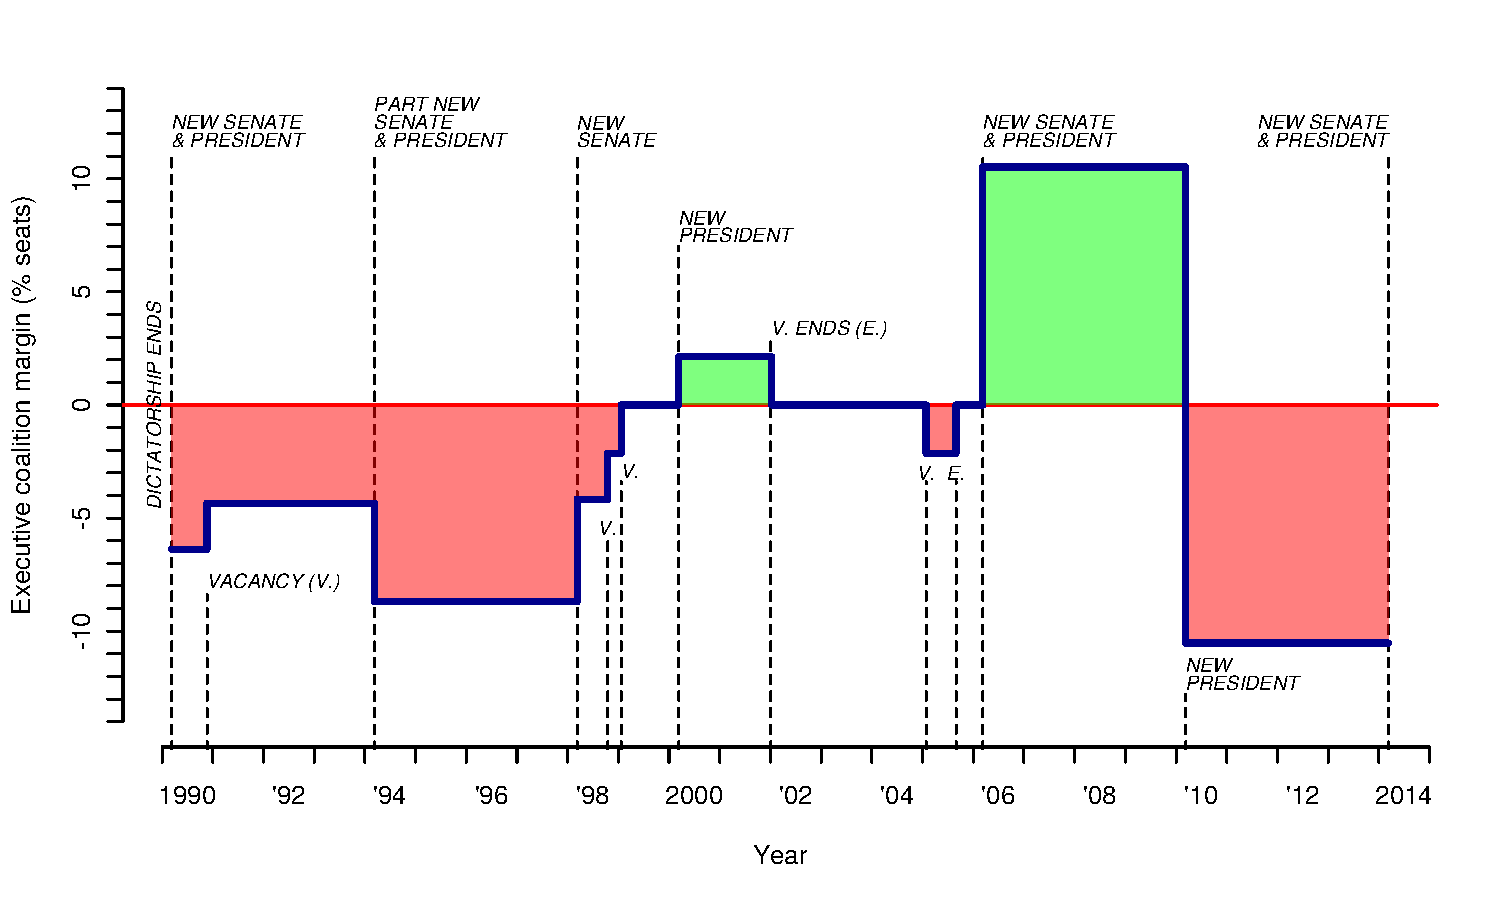
\includegraphics[width=\columnwidth]{../graphs/senChile.pdf}
%% %   \caption{The Conservative chamber. The blue, crenellated line reports, longitudinally, the percentage of Senate seats controlled by the president's coalition minus the percentage controlled by the opposition. Totals include 38 elected senators and, up to 2006, 9 appointed senators and two or less senators for life. Vacancies, if any, are excluded from the denominator (see text). A new Senate is elected every eight years, and was partially renewed in 1994. Vacancies in the period: Ruiz Danyau, Air Force appointee, died in office 11/1990; Pinochet detained in London 10/1998; Errázuriz stripped of immunity 1/1999 (resinstated 1/2002); Lavandero stripped of immunity 1/2005 (replaced upon conviction 8/2005). }\label{f:senChile}
%% % \end{center}
%% % \end{figure}



%% % % \begin{tabular}{lrrrrrr}
%% % %                                   &  \mc{2}{c}{passed}    &  \mc{2}{c}{not}     &  \mc{2}{c}{all}      \\    
%% % % Bills with urgency in             &  N     &  \%          &  N     &  \%        &  N     &  \%         \\ \hline
%% % % $1^{st}$ chamber only              &   122  &  \emph{32}   &   259  &  \emph{68} &   381  &  \emph{100} \\
%% % % $2^{nd}$ chamber only              &   129  &  \emph{68}   &    62  &  \emph{32} &   191  &  \emph{100} \\
%% % % conference only                   &    27  &  \emph{82}   &     6  &  \emph{18} &    33  &  \emph{100} \\
%% % % $1^{st}$ and $2^{nd}$               &   363  &  \emph{81}   &    87  &  \emph{19} &   450  &  \emph{100} \\
%% % % $1^{st}$ and conference            &    39  &  \emph{93}   &     3  &  \emph{7}  &    42  &  \emph{100} \\
%% % % $2^{nd}$ and conference            &    37  &  \emph{90}   &     4  &  \emph{10} &    41  &  \emph{100} \\
%% % % $1^{st}$, $2^{nd}$, and conference  &   212  &  \emph{94}   &    14  &  \emph{6}  &   226  &  \emph{100} \\
%% % % no urgency                        &   541  &  \emph{10}   &  5097  &  \emph{90} &   5638 &  \emph{100} \\ \hline
%% % % %total                             &   929  &  \emph{68}   &   435  &  \emph{32} &  1364  &  \emph{100} \\ \hline
%% % % \end{tabular}

%% % An urgency message can be sent at any stage of the bicameral legislative process, compelling the chamber receiving it to act on a bill. Since urgencies expire once the chamber has finished, it is not uncommon for presidents to send messages at more than one step. Two-fifths of bills with urgencies were deemed so in two or three steps of the legislative process---the first chamber, the second, and/or the bicameral conference.    

%% % % \begin{table}
%% % % \begin{center}
%% % % \begin{tabular}{lrrr|rrr}
%% % %                                   &  \mc{6}{c}{Proposer}                                               \\    
%% % %                                   &  \mc{3}{c}{president}         &  \mc{3}{c}{member of Congress}             \\    
%% % % Bills with urgency in             &  \% pass   & \% not    & ~~~~~N &  \% pass  & \% not    & ~~~~~N \\ \hline
%% % % $1^{st}$ chamber only              &  \emph{40} & \emph{60} & 278  & \emph{12} & \emph{88} & 103  \\
%% % % $2^{nd}$ chamber only              &  \emph{84} & \emph{16} &  98  & \emph{51} & \emph{49} &  93  \\
%% % % conference only                   &  \emph{95} & \emph{5}  &  20  & \emph{62} & \emph{38} &  13  \\
%% % % $1^{st}$ and $2^{nd}$               &  \emph{86} & \emph{14} & 369  & \emph{58} & \emph{42} &  81  \\
%% % % $1^{st}$ and conference            &  \emph{92} & \emph{8}  &  39  & \emph{100}& \emph{0}  &   3  \\
%% % % $2^{nd}$ and conference            &  \emph{100}& \emph{0}  &  18  & \emph{83} & \emph{17} &  23  \\
%% % % $1^{st}$, $2^{nd}$, and conference  &  \emph{94} & \emph{6}  & 192  & \emph{91} & \emph{9}  &  34  \\
%% % % no urgency                        &  \emph{67} & \emph{33} & 455  & \emph{5}  & \emph{95} & 5183  \\ \hline
%% % % \end{tabular}
%% % % \caption{The legislative process, urgency messages, and bill passage by proposer 1998--2014}\label{T:stepsUrgencyPass}
%% % % \end{center}
%% % % \end{table}

%% % \begin{table}
%% % \begin{center}
%% % \begin{tabular}{lrrr|rrr}
%% %                        &  \mc{6}{c}{Proposer}                                               \\    
%% % Step(s) with           &  \mc{3}{c}{president}         &  \mc{3}{c}{member of Congress}             \\    
%% % urgency declared       &  \% pass    & \% not      & ~~~~~N &  \% pass  & \% not      & ~~~~~N \\ \hline
%% % 1 only                 &  \emph{41}  &  \emph{59}  &  285 &  \emph{12}  &  \emph{88}  &  103 \\
%% % 2 only                 &  \emph{84}  &  \emph{16}  &  102 &  \emph{52}  &  \emph{48}  &  96  \\
%% % 3 only                 &  \emph{90}  &  \emph{10}  &  10  &  \emph{75}  &  \emph{25}  &  4   \\
%% % $c$ only               &  \emph{100} &  \emph{0}   &  8   &  \emph{57}  &  \emph{43}  &  7   \\
%% % 1 and 2                &  \emph{85}  &  \emph{15}  &  382 &  \emph{60}  &  \emph{40}  &  84  \\
%% % two of more            &  \emph{100} &  \emph{0}   &  37  &  \emph{90}  &  \emph{10}  &  21  \\
%% % 1, 2, and 3            &  \emph{94}  &  \emph{6}   &  89  &  \emph{90}  &  \emph{10}  &  10  \\
%% % three of more          &  \emph{96}  &  \emph{4}   &  55  &  \emph{86}  &  \emph{14}  &  14  \\
%% % 1, 2, 3, and $c$       &  \emph{93}  &  \emph{7}   &  44  &  \emph{80}  &  \emph{20}  &  10  \\
%% % no urgency             &  \emph{67}  &  \emph{33}  &  457 &  \emph{5}   &  \emph{95}  &  5184 \\ \hline
%% % \end{tabular}
%% % \caption{Legislative steps, urgency messages, and bill passage by proposer 1998--2014. Steps are coded thus: 1 for the chamber of origin, 2 for the revising chamber, 3 for the chamber of origin's response, and $c$ for the conference committee. Cells report bill frequencies.}\label{T:stepsUrgencyPass}
%% % \end{center}
%% % \end{table}







%% % \section{Discussion}

%% % The more difficult it is for an assembly to form and maintain majorities capable of passing legislation, the more attractive it becomes to delegate responsibility to the executive.  Specific examples of situations where decrees may become more attractive are systems where legislative parties have a chronic incapacity to discipline members (as in Brazil), or bicameral systems where malapportionment typically produces majorities of different parties in each house, as in Chile before the removal of appointed senators in 2006 \citep[see][]{carey.shugart.1998a,cox.mccubbins.2001}.

%% % A theme worth pursuing are the determinants of unilateralism.  The logic behind executive vetoes (a concurrent consent institution) extends naturally to executive decrees (a restricted unilateralism institution). In the Linzian framework,\footnote{``[T]here is no democratic principle to resolve [conflict]'' \citeyear[][7]{linz.1994}.} unilateralism appears as unconstitutional moves by the executive to bypass the legislature in the context of impasse---an indicator of deep polarization (also O'Donnell). Presidential unilateralism is tantamount to a democratic system overheating dangerously, perhaps ready to melt into authoritarianism.  The factor driving decree incidence is, again, polarization between the branches. Is there evidence? 

%% % Because it pays attention to a single case giving no constitutional decree authority to its president, Cameron's work remains silent about executive unilateralism.  But following the logic of the bargaining approach, decrees should simply represent one additional tool that the president can resort to in his or her quest for influence on policy.  The veto power has a ``second face'' pointing to silent influence through a capacity of players to anticipate each other's acts; uncertainty reduces that capacity, prompting mistakes and a strategic use of them to gain reputations of toughness in bargaining \citep{cameron.2000,mccarty.1997}.  In the same fashion the decree power hides a second face (e.g. Congress makes a slightly larger concession to the president to avoid a decree of his or hers), and to the extent that players have incomplete information, some should occur and be rescinded as mistakes and reputation-building maneuvers.  

%% % Decrees can also be construed as part of a position-taking game.  It seems plausible that a president decrees some policy knowing, beforehand, that it will be rescinded by the assembly.  The intention is to force the assembly to reject policy popular to his constituents, increase the salience of the issue, and subsequently exploit this when campaigning (or give fellow party members a banner to fly in their campaigns).  Similarly, the assembly may concoct a bill attempting to avoid an executive decree modifying it; in doing so it may miscalculate and make insufficient concessions to the president, prompting the decree which legislators meant to avoid.  



%% \section{Closing remarks}

%% Inspection of urgency message predictors and committee reporting within the time frame that presidential messages set forth has uncovered evidence consistent with consequential urgency authority in Chile. The paper is far from conclusive, however: other than raising an abstract cost of ignoring urgent calls, why members of Congress heed executive cheap talk remains a puzzle. But patterns in the data suggest a promising area for research.  

%% % %% version without urgency step
%% % \begin{sidewaysfigure}
%% % \centering
%% % \begin{tabular}{cc}
%% % %\textbf{Executive-initiated bills} & \textbf{MC-initiated bills} \\
%% % \textbf{Piñera bills sent to Cámara} & \textbf{Piñera bills sent to Senate} \\
%% % ($N=314$) & ($N=90$) \\
%% % \tikzstyle{mid}=[circle,draw]
%% % \tikzstyle{middot}=[circle,draw,dashed]
%% % \begin{tikzpicture}[shorten >=1pt,node distance=2cm,auto,scale=.6]
%% % %\draw[help lines] (-6,-6) grid (6,6);
%% % \node at (-4,6) (st) {\footnotesize{\textbf{\texttt{start}}}};
%% % \node[mid]     at (0,0)   (p)  {\textbf{Exec.}};
%% % \node[mid,green] at (0,6)   (n1) {\textbf{Cám.}};
%% % \node[mid,red]   at (6,0)   (n2) {\textbf{Sen.}};
%% % \node[mid,green] at (0,-6)  (n3) {\textbf{Cám.}};
%% % \node[mid]       at (-6,0)  (c)  {\textbf{Conf.}};
%% % %\node[middot]    at (2,3)   (u)  {$u$};
%% % %\node[middot]    at (3,-2)  (v)  {$u$};
%% % %\node[middot]    at (-2,-3) (w)  {$u$};
%% % %\node[middot]    at (-3,2)  (x)  {$u$};
%% % \draw [-stealth] (st)                    edge node {100} (n1);
%% % \draw [-stealth] (n1) [loop above]       edge node              {22} ();    % l11 $A$
%% % %\draw [-stealth] (n1) [bend left,dashed] edge node              {75} (u);   % l1u $B$
%% % \draw [-stealth] (n1) [out=0,in=90]      edge node              {78} (n2);  % l12 $C$
%% % %\draw [-stealth] (u)  [bend left]        edge node              {14} (n1);  % lu1 $D$
%% % %\draw [-stealth] (u)                     edge node              {61} (n2);  % lu2 $E$
%% % \draw [-stealth] (n2) [loop right]       edge node              {10} ();    % l22 $F$
%% % \draw [-stealth] (n2) [out=-90,in=0]     edge node              {31} (n3);  % l23 $G$
%% % %\draw [-stealth] (n2) [bend left,dashed] edge node              {57} (v);   % l2v $H$
%% % \draw [-stealth] (n2) [out=170, in=10]   edge node [swap]       {36} (p);   % l2p $I$
%% % %\draw [-stealth] (v)  [bend left]        edge node              { 7} (n2);  % lv2 $J$
%% % %\draw [-stealth] (v)                     edge node [swap]       {24} (p)    % lvp $K$
%% % %                 (v)                     edge node              {25} (n3);  % lv3 $L$
%% % \draw [-stealth] (n3) [loop below]       edge node              { 0} ();    % l33 $N$
%% % \draw [-stealth] (n3) [out=180,in=-90]   edge node              { 7} (c);   % l3c $O$
%% % %\draw [-stealth] (n3) [bend left,dashed] edge node              {11} (w);   % l3w $P$
%% % \draw [-stealth] (n3) [out=80, in=-80]   edge node [swap]       {24} (p);   % l3p $Q$
%% % %\draw [-stealth] (w)  [bend left]        edge node [near start] { 0} (n3);  % lw3 $R$
%% % %\draw [-stealth] (w)                     edge node              { 9} (p)    % lwp $S$
%% % %                 (w)                     edge node              { 1} (c);   % lwc $U$
%% % \draw [-stealth] (c)  [loop left]        edge node              { 0} ();    % lcc $V$
%% % %\draw [-stealth] (c)  [bend left,dashed] edge node              { 5} (x);   % lcx $W$
%% % \draw [-stealth] (c)  [out=-10, in=-170] edge node [swap]       { 7} (p);   % lcp $X$
%% % %\draw [-stealth] (x)  [bend left]        edge node              { 0} (c);   % lxc $Y$
%% % %\draw [-stealth] (x)                     edge node              { 5} (p);   % lcp $Z$
%% % \end{tikzpicture}
%% % &
%% % \tikzstyle{mid}=[circle,draw]
%% % \tikzstyle{middot}=[circle,draw,dashed]
%% % \begin{tikzpicture}[shorten >=1pt,node distance=2cm,auto,scale=.6]
%% % %\draw[help lines] (-6,-6) grid (6,6);
%% % \node at (-4,6) (st) {\footnotesize{\textbf{\texttt{start}}}};
%% % \node[mid]       at (0,0)   (p)  {\textbf{Exec.}};
%% % \node[mid,red]   at (0,6)   (n1) {\textbf{Sen.}};
%% % \node[mid,green] at (6,0)   (n2) {\textbf{Cám.}};
%% % \node[mid,red]   at (0,-6)  (n3) {\textbf{Sen.}};
%% % \node[mid]       at (-6,0)  (c)  {\textbf{Conf.}};
%% % %\node[middot]    at (2,3)   (u)  {$u$};
%% % %\node[middot]    at (3,-2)  (v)  {$u$};
%% % %\node[middot]    at (-2,-3) (w)  {$u$};
%% % %\node[middot]    at (-3,2)  (x)  {$u$};
%% % \draw [-stealth] (st)                    edge node {100} (n1);
%% % \draw [-stealth] (n1) [loop above]       edge node              {39} ();    % l11 $A$
%% % %\draw [-stealth] (n1) [bend left,dashed] edge node              {79} (u);   % l1u $B$
%% % \draw [-stealth] (n1) [out=0,in=90]      edge node              {61} (n2);  % l12 $C$
%% % %\draw [-stealth] (u)  [bend left]        edge node              {31} (n1);  % lu1 $D$
%% % %\draw [-stealth] (u)                     edge node              {48} (n2);  % lu2 $E$
%% % \draw [-stealth] (n2) [loop right]       edge node              { 7} ();    % l22 $F$
%% % \draw [-stealth] (n2) [out=-90,in=0]     edge node              {29} (n3);  % l23 $G$
%% % %\draw [-stealth] (n2) [bend left,dashed] edge node              {47} (v);   % l2v $H$
%% % \draw [-stealth] (n2) [out=170, in=10]   edge node [swap]       {26} (p);   % l2p $I$
%% % %\draw [-stealth] (v)  [bend left]        edge node              { 6} (n2);  % lv2 $J$
%% % %\draw [-stealth] (v)                     edge node [swap]       {18} (p)    % lvp $K$
%% % %                 (v)                     edge node              {23} (n3);  % lv3 $L$
%% % \draw [-stealth] (n3) [loop below]       edge node              { 0} ();    % l33 $N$
%% % \draw [-stealth] (n3) [out=180,in=-90]   edge node              {11} (c);   % l3c $O$
%% % %\draw [-stealth] (n3) [bend left,dashed] edge node              {18} (w);   % l3w $P$
%% % \draw [-stealth] (n3) [out=80, in=-80]   edge node [swap]       {18} (p);   % l3p $Q$
%% % %\draw [-stealth] (w)  [bend left]        edge node [near start] { 0} (n3);  % lw3 $R$
%% % %\draw [-stealth] (w)                     edge node              {11} (p)    % lwp $S$
%% % %                 (w)                     edge node              { 7} (c);   % lwc $U$
%% % \draw [-stealth] (c)  [loop left]        edge node              { 2} ();    % lcc $V$
%% % %\draw [-stealth] (c)  [bend left,dashed] edge node              { 8} (x);   % lcx $W$
%% % \draw [-stealth] (c)  [out=-10, in=-170] edge node [swap]       { 9} (p);   % lcp $X$
%% % %\draw [-stealth] (x)  [bend left]        edge node              { 1} (c);   % lxc $Y$
%% % %\draw [-stealth] (x)                     edge node              { 7} (p);   % lcp $Z$
%% % \end{tikzpicture}
%% % \\
%% % \end{tabular}
%% % \caption{Paths of executive bills in Congress. Cám.\, Sen.\, Conf.\, and Exec.\ refer to Cámara de Diputados, Senate, Conference committee, and executive's desk. Numbers are all relative to base 100 (ie., frequency*100/total bills), rounded to nearest integer.}\label{F:billPaths}
%% % \end{sidewaysfigure}

%% %% version with urgency step
%% \begin{sidewaysfigure}%\ContinuedFloat
%% \centering
%% \begin{tabular}{cc}
%% %\textbf{Executive-initiated bills} & \textbf{MC-initiated bills} \\
%% \textbf{Piñera bills sent to Cámara} & \textbf{Piñera bills sent to Senate} \\
%% ($N=314$) & ($N=90$) \\
%% \tikzstyle{mid}=[circle,draw]
%% \tikzstyle{middot}=[circle,draw,dashed]
%% \begin{tikzpicture}[shorten >=1pt,node distance=2cm,auto,scale=.6]
%% %\draw[help lines] (-6,-6) grid (6,6);
%% \node at (-4,6) (st) {\footnotesize{\textbf{\texttt{start}}}};
%% \node[mid]     at (0,0)   (p)  {\textbf{Exec.}};
%% \node[mid,green] at (0,6)   (n1) {\textbf{Cám.}};
%% \node[mid,red]   at (6,0)   (n2) {\textbf{Sen.}};
%% \node[mid,green] at (0,-6)  (n3) {\textbf{Cám.}};
%% \node[mid]       at (-6,0)  (c)  {\textbf{Conf.}};
%% \node[middot]    at (2,3)   (u)  {$u$};
%% \node[middot]    at (3,-2)  (v)  {$u$};
%% \node[middot]    at (-2,-3) (w)  {$u$};
%% \node[middot]    at (-3,2)  (x)  {$u$};
%% \draw [-stealth] (st)                    edge node {100} (n1);
%% \draw [-stealth] (n1) [loop above]       edge node              { 8} ();    % l11 $A$
%% \draw [-stealth] (n1) [bend left,dashed] edge node              {75} (u);   % l1u $B$
%% \draw [-stealth] (n1) [out=0,in=90]      edge node              {17} (n2);  % l12 $C$
%% \draw [-stealth] (u)  [bend left]        edge node              {14} (n1);  % lu1 $D$
%% \draw [-stealth] (u)                     edge node              {61} (n2);  % lu2 $E$
%% \draw [-stealth] (n2) [loop right]       edge node              { 3} ();    % l22 $F$
%% \draw [-stealth] (n2) [out=-90,in=0]     edge node              { 6} (n3);  % l23 $G$
%% \draw [-stealth] (n2) [bend left,dashed] edge node              {57} (v);   % l2v $H$
%% \draw [-stealth] (n2) [out=170, in=10]   edge node [swap]       {12} (p);   % l2p $I$
%% \draw [-stealth] (v)  [bend left]        edge node              { 7} (n2);  % lv2 $J$
%% \draw [-stealth] (v)                     edge node [swap]       {24} (p)    % lvp $K$
%%                  (v)                     edge node              {25} (n3);  % lv3 $L$
%% \draw [-stealth] (n3) [loop below]       edge node              { 0} ();    % l33 $N$
%% \draw [-stealth] (n3) [out=180,in=-90]   edge node              { 6} (c);   % l3c $O$
%% \draw [-stealth] (n3) [bend left,dashed] edge node              {11} (w);   % l3w $P$
%% \draw [-stealth] (n3) [out=80, in=-80]   edge node [swap]       {15} (p);   % l3p $Q$
%% \draw [-stealth] (w)  [bend left]        edge node [near start] { 0} (n3);  % lw3 $R$
%% \draw [-stealth] (w)                     edge node              { 9} (p)    % lwp $S$
%%                  (w)                     edge node              { 1} (c);   % lwc $U$
%% \draw [-stealth] (c)  [loop left]        edge node              { 0} ();    % lcc $V$
%% \draw [-stealth] (c)  [bend left,dashed] edge node              { 5} (x);   % lcx $W$
%% \draw [-stealth] (c)  [out=-10, in=-170] edge node [swap]       { 2} (p);   % lcp $X$
%% \draw [-stealth] (x)  [bend left]        edge node              { 0} (c);   % lxc $Y$
%% \draw [-stealth] (x)                     edge node              { 5} (p);   % lcp $Z$
%% \end{tikzpicture}
%% &
%% \tikzstyle{mid}=[circle,draw]
%% \tikzstyle{middot}=[circle,draw,dashed]
%% \begin{tikzpicture}[shorten >=1pt,node distance=2cm,auto,scale=.6]
%% %\draw[help lines] (-6,-6) grid (6,6);
%% \node at (-4,6) (st) {\footnotesize{\textbf{\texttt{start}}}};
%% \node[mid]       at (0,0)   (p)  {\textbf{Exec.}};
%% \node[mid,red]   at (0,6)   (n1) {\textbf{Sen.}};
%% \node[mid,green] at (6,0)   (n2) {\textbf{Cám.}};
%% \node[mid,red]   at (0,-6)  (n3) {\textbf{Sen.}};
%% \node[mid]       at (-6,0)  (c)  {\textbf{Conf.}};
%% \node[middot]    at (2,3)   (u)  {$u$};
%% \node[middot]    at (3,-2)  (v)  {$u$};
%% \node[middot]    at (-2,-3) (w)  {$u$};
%% \node[middot]    at (-3,2)  (x)  {$u$};
%% \draw [-stealth] (st)                    edge node {100} (n1);
%% \draw [-stealth] (n1) [loop above]       edge node              { 8} ();    % l11 $A$
%% \draw [-stealth] (n1) [bend left,dashed] edge node              {79} (u);   % l1u $B$
%% \draw [-stealth] (n1) [out=0,in=90]      edge node              {13} (n2);  % l12 $C$
%% \draw [-stealth] (u)  [bend left]        edge node              {31} (n1);  % lu1 $D$
%% \draw [-stealth] (u)                     edge node              {48} (n2);  % lu2 $E$
%% \draw [-stealth] (n2) [loop right]       edge node              { 1} ();    % l22 $F$
%% \draw [-stealth] (n2) [out=-90,in=0]     edge node              { 6} (n3);  % l23 $G$
%% \draw [-stealth] (n2) [bend left,dashed] edge node              {47} (v);   % l2v $H$
%% \draw [-stealth] (n2) [out=170, in=10]   edge node [swap]       { 8} (p);   % l2p $I$
%% \draw [-stealth] (v)  [bend left]        edge node              { 6} (n2);  % lv2 $J$
%% \draw [-stealth] (v)                     edge node [swap]       {18} (p)    % lvp $K$
%%                  (v)                     edge node              {23} (n3);  % lv3 $L$
%% \draw [-stealth] (n3) [loop below]       edge node              { 0} ();    % l33 $N$
%% \draw [-stealth] (n3) [out=180,in=-90]   edge node              { 4} (c);   % l3c $O$
%% \draw [-stealth] (n3) [bend left,dashed] edge node              {18} (w);   % l3w $P$
%% \draw [-stealth] (n3) [out=80, in=-80]   edge node [swap]       { 7} (p);   % l3p $Q$
%% \draw [-stealth] (w)  [bend left]        edge node [near start] { 0} (n3);  % lw3 $R$
%% \draw [-stealth] (w)                     edge node              {11} (p)    % lwp $S$
%%                  (w)                     edge node              { 7} (c);   % lwc $U$
%% \draw [-stealth] (c)  [loop left]        edge node              { 1} ();    % lcc $V$
%% \draw [-stealth] (c)  [bend left,dashed] edge node              { 8} (x);   % lcx $W$
%% \draw [-stealth] (c)  [out=-10, in=-170] edge node [swap]       { 2} (p);   % lcp $X$
%% \draw [-stealth] (x)  [bend left]        edge node              { 1} (c);   % lxc $Y$
%% \draw [-stealth] (x)                     edge node              { 7} (p);   % lcp $Z$
%% \end{tikzpicture}
%% \\
%% \end{tabular}
%% %\caption{Paths of executive bills (cont.\ distinguishing urgencies)}
%% \caption{Paths of executive bills in Congress 2010--14. Cám.\, Sen.\, Conf.\, and Exec.\ refer to Cámara de Diputados, Senate, Conference committee, and executive's desk, respectively. Numbers are all relative to base 100 (i.e., freq.$\times$100/\emph{N}), rounded to nearest integer.}\label{F:billPaths}
%% \end{sidewaysfigure}

%% The big challenge is a method to deal with the selection problem complicating analysis of the urgency--bill passage relation. I close with a look at the bigger picture to give an idea of this obstacle. Figure \ref{F:billPaths} follows President Piñera's proposals ($N=394$) along the full bicameral legislative process, keeping Cámara- (left panel) and Senate-initiated bills (right) separate. The diagram reports relative numbers of proposals in the different paths (atop arrows), distinguishing proposals that proceeded to the next node (i.e., bills that passed, possibly amended) from those that did not (bills rejected, pending, or never considered). It also separates bills that became urgent (the dashed paths) from those that did not. Plots show that urgencies cannot always overcome obstacles in the process. Piñera faced an opposition-controlled Senate throughout his term, yet declared similar proportions of Cámara- and Senate-initiated bills urgent (75 and 79 percent, respectively). The key difference is related to presidential anticipation of rougher terrain in the upper chamber, Piñera sending four out of five proposals to the Cámara. Those he did sent to the Senate were, in fact, less likely to proceed to the next node than the Cámara-initiated ($17+61=78$ v\ $13+48=61$ percent). Also noteworthy is that half as many urgencies in the Cámara failed to move the bill forward compared to the Senate  (14 v 31 percent). If urgency messages trigger reports to the Congressional floor in predictable ways, they are certainly no guarantee of executive success: two out of five urgent Senate-initiated bills ($31/79$) never reached the revising stage, and one-fith in the lower chamber ($14/75$). Few chamber of origin differences arised once legislation reached the second node (relative to the traffic arriving there). Only the shares of bills amended in revising chamber, and therefore sent back to the originating, are somewhat different ($(25+6)/78=.4$ for Cámara-initiated bills, $(23+6)/61=.48$ for Senate-initiated bills). Differences arise again in the third node (when the originating chamber can either concur with amendments by the revising or proceed to conference). Interestingly, the share of urgent bills in third node not proceeding further collapses to zero, regardless of chamber of origin. But the proportion of urgent Senate-initiated bills ($18/(23+6)=.62$) was substantially higher than the Cámara-initiated ($11/(25+6)=.35$). Urgency and success are more strongly associated at later stages of the legislative process. 

%% The urgency authority in the continent is an institution worth studying more carefully. The next chapter inspects it in Brazil, where it is related to executive unilaterlism. Unlike Chile's, the Brazilian reversionary outcome and agenda play in favor of executive influence, simplifying analysis considerably.

%% %To stimulate debate, I close with a bigger picture of the urgency--bill passage relation. Figure \ref{F:billPaths} follows 394 proposals by President Piñera along the bicameral legislative process. Facing an opposition-controlled Senate throughout his term, Piñera chose to send four out of five bills to the Cámara. The diagram reports relative numbers of proposals in the different paths (atop arrows), distinguishing proposals that proceeded to the next chamber (i.e., bills that passed, possibly amended) from those that did not (bills rejected, pending, or never considered). It also separates bills that became urgent (the dashed paths) from those that did not. Initial differences across chambers are notable: if shares of bills tagged urgent in the Cámara and Senate are very similar (75 and 79 percent, respectively), nearly one-fifth more proceeded to the next node in the former than the latter ($17+61=78$ vs.\ $13+48=61$ percent). The failure differential may explain the executive's preference for lower-chamber initiation, but not why Piñera still chose to initiate 90 bills in the Senate. Also noteworthy is that half as many urgencies in the Cámara failed to move the bill forward compared to the Senate  (14 and 31 percent, respectively). If, as seen in the chapter, urgency messages trigger movement in Congress in predictable ways, they are certainly no guarantee of executive success: two out of five urgent bills in the Senate ($31/79$) never reached the Cámara, one-fith in the lower chamber ($14/75$) did not make it to the Senate. Moving to the next node in the legislative process reveals that most inter-chamber differences vanish in the revising chamber: proportions of bills passed unamended by the second chamber and therefore sent to the executive's desk are similar ($(12+24=36)/78=.46$ for Cámara-initiated proposals and $(8+18=26)/61=.43$ for the Senate-initiated), as are shares of proposals declared urgent ($57/78=.73$ and $47/61=.77$, respectively) and shares of urgencies failing to push the bill forward ($7/57=.12$ and $6/47=.13$, respectively). Only the shares of bills amended in second chamber and therefore sent back to the originating chamber change slightly ($(25+6)/78=.4$ for Cámara-initiated bills, $(23+6)/61=.48$ for Senate-initiated bills). And differences reappear further down, the originating chamber concurring with amendments more often in Cámara- than in Senate-initiated bills (.77 v .62), less bills calling for urgency (.35 v .62), and fewer going to conference. While the urgency authority is certainly related to success, it is hardly determinant. 


%% % \section{Online appendix}
%% %
%% % Bill urgency logit models. 
%% %
%% % \begin{verbatim}
%% % > summary(fit1)
%% %
%% % Call:
%% % glm(formula = dv ~ dmocion + drefHda + dmajSen + dinSen + ptermR + 
%% %     legyrR + dreform2010, family = binomial(link = logit), data = tmpdat)
%% %
%% % Deviance Residuals: 
%% %     Min       1Q   Median       3Q      Max  
%% % -2.2416  -0.3734  -0.3311  -0.2942   2.5993  
%% %
%% % Coefficients:
%% %             Estimate Std. Error z value Pr(>|z|)    
%% % (Intercept)  0.11684    0.16082   0.727   0.4675    
%% % dmocion     -2.98974    0.09096 -32.868   <2e-16 ***
%% % drefHda      1.76145    0.11077  15.902   <2e-16 ***
%% % dmajSen     -0.12186    0.15900  -0.766   0.4434    
%% % dinSen       0.18243    0.09609   1.898   0.0576 .  
%% % ptermR       0.10363    0.04195   2.470   0.0135 *  
%% % legyrR       0.07784    0.04228   1.841   0.0656 .  
%% % dreform2010  0.22938    0.16788   1.366   0.1718    
%% % ---
%% % Signif. codes:  0 ‘***’ 0.001 ‘**’ 0.01 ‘*’ 0.05 ‘.’ 0.1 ‘ ’ 1
%% %
%% % (Dispersion parameter for binomial family taken to be 1)
%% %
%% %     Null deviance: 6893.3  on 6986  degrees of freedom
%% % Residual deviance: 4111.3  on 6979  degrees of freedom
%% % AIC: 4127.3
%% %
%% % Number of Fisher Scoring iterations: 5
%% %
%% % > summary(fit2)
%% %
%% % Call:
%% % glm(formula = dv ~ dmocionAllOpp + dmocionMix + dmocionAllPdt + 
%% %     drefHda + dmajSen + dinSen + ptermR + legyrR + dreform2010, 
%% %     family = binomial(link = logit), data = tmpdat)
%% %
%% % Deviance Residuals: 
%% %     Min       1Q   Median       3Q      Max  
%% % -2.3227  -0.3973  -0.3235  -0.2243   2.7781  
%% %
%% % Coefficients:
%% %               Estimate Std. Error z value Pr(>|z|)    
%% % (Intercept)    0.11287    0.16244   0.695 0.487163    
%% % dmocionAllOpp -3.60272    0.13728 -26.244  < 2e-16 ***
%% % dmocionMix    -2.53044    0.11534 -21.939  < 2e-16 ***
%% % dmocionAllPdt -2.97420    0.12626 -23.557  < 2e-16 ***
%% % drefHda        1.78289    0.11134  16.014  < 2e-16 ***
%% % dmajSen       -0.16221    0.16069  -1.009 0.312758    
%% % dinSen         0.41216    0.11095   3.715 0.000203 ***
%% % ptermR         0.11042    0.04231   2.610 0.009066 ** 
%% % legyrR         0.08018    0.04246   1.888 0.058985 .  
%% % dreform2010    0.17586    0.16987   1.035 0.300545    
%% % ---
%% % Signif. codes:  0 ‘***’ 0.001 ‘**’ 0.01 ‘*’ 0.05 ‘.’ 0.1 ‘ ’ 1
%% %
%% % (Dispersion parameter for binomial family taken to be 1)
%% %
%% %     Null deviance: 6893.3  on 6986  degrees of freedom
%% % Residual deviance: 4057.5  on 6977  degrees of freedom
%% % AIC: 4077.5
%% %
%% % Number of Fisher Scoring iterations: 6
%% %
%% % > summary(fit3)
%% %
%% % Call:
%% % glm(formula = dv ~ dmocionAllOpp + dmocionMix + dmocionAllPdt + 
%% %     drefHda + dmajSen + dinSen + ptermR + legyrR + dreform2010 + 
%% %     as.factor(legis), family = binomial(link = logit), data = tmpdat)
%% %
%% % Deviance Residuals: 
%% %     Min       1Q   Median       3Q      Max  
%% % -2.3350  -0.4107  -0.3142  -0.2291   2.9115  
%% %
%% % Coefficients:
%% %                      Estimate Std. Error z value Pr(>|z|)    
%% % (Intercept)           0.26152    0.21057   1.242  0.21425    
%% % dmocionAllOpp        -3.70649    0.14072 -26.339  < 2e-16 ***
%% % dmocionMix           -2.64589    0.11967 -22.109  < 2e-16 ***
%% % dmocionAllPdt        -3.07657    0.13046 -23.582  < 2e-16 ***
%% % drefHda               1.75917    0.11215  15.686  < 2e-16 ***
%% % dmajSen              -0.37065    0.20868  -1.776  0.07570 .  
%% % dinSen                0.39545    0.11149   3.547  0.00039 ***
%% % ptermR                0.08349    0.04646   1.797  0.07235 .  
%% % legyrR                0.08452    0.04279   1.975  0.04825 *  
%% % dreform2010           0.17376    0.28896   0.601  0.54764    
%% % as.factor(legis)2002 -0.23155    0.15496  -1.494  0.13512    
%% % as.factor(legis)2006  0.33323    0.14608   2.281  0.02254 *  
%% % as.factor(legis)2010 -0.06295    0.35112  -0.179  0.85771    
%% % ---
%% % Signif. codes:  0 ‘***’ 0.001 ‘**’ 0.01 ‘*’ 0.05 ‘.’ 0.1 ‘ ’ 1
%% %
%% % (Dispersion parameter for binomial family taken to be 1)
%% %
%% %     Null deviance: 6893.3  on 6986  degrees of freedom
%% % Residual deviance: 4037.8  on 6974  degrees of freedom
%% % AIC: 4063.8
%% %
%% % Number of Fisher Scoring iterations: 6
%% %
%% % > summary(fit4)
%% % Generalized linear mixed model fit by maximum likelihood (Laplace Approximation) ['glmerMod']
%% %  Family: binomial  ( logit )
%% % Formula: dv ~ dmocionAllOpp + dmocionMix + dmocionAllPdt + drefHda + dmajSen +      dinSen + ptermR + legyrR + dreform2010 + (1 | legis)
%% %    Data: tmpdat
%% %
%% %      AIC      BIC   logLik deviance df.resid 
%% %   4070.5   4145.9  -2024.3   4048.5     6976 
%% %
%% % Scaled residuals: 
%% %     Min      1Q  Median      3Q     Max 
%% % -3.7614 -0.2940 -0.2263 -0.1634  7.9304 
%% %
%% % Random effects:
%% %  Groups Name        Variance Std.Dev.
%% %  legis  (Intercept) 0.03167  0.1779  
%% % Number of obs: 6987, groups:  legis, 4
%% %
%% % Fixed effects:
%% %               Estimate Std. Error z value Pr(>|z|)    
%% % (Intercept)    0.23385    0.19175   1.220 0.222616    
%% % dmocionAllOpp -3.68591    0.14074 -26.190  < 2e-16 ***
%% % dmocionMix    -2.62186    0.11990 -21.868  < 2e-16 ***
%% % dmocionAllPdt -3.05558    0.13038 -23.436  < 2e-16 ***
%% % drefHda        1.76379    0.11203  15.743  < 2e-16 ***
%% % dmajSen       -0.30920    0.18177  -1.701 0.088925 .  
%% % dinSen         0.39843    0.11135   3.578 0.000346 ***
%% % ptermR         0.08657    0.04425   1.956 0.050428 .  
%% % legyrR         0.08324    0.04269   1.950 0.051202 .  
%% % dreform2010    0.13795    0.20817   0.663 0.507523    
%% % ---
%% % Signif. codes:  0 ‘***’ 0.001 ‘**’ 0.01 ‘*’ 0.05 ‘.’ 0.1 ‘ ’ 1
%% %
%% % Correlation of Fixed Effects:
%% %             (Intr) dmcnAO dmcnMx dmcnAP drefHd dmajSn dinSen ptermR legyrR
%% % dmocnAllOpp -0.204                                                        
%% % dmocionMix  -0.255  0.324                                                 
%% % dmocnAllPdt -0.193  0.399  0.320                                          
%% % drefHda     -0.211  0.167  0.250  0.189                                   
%% % dmajSen     -0.766  0.076  0.056  0.058  0.026                            
%% % dinSen      -0.114 -0.223  0.184 -0.336  0.065  0.009                     
%% % ptermR       0.104 -0.093 -0.080 -0.055  0.040 -0.117 -0.018              
%% % legyrR      -0.130 -0.038 -0.043 -0.014  0.042  0.147  0.011 -0.146       
%% % dreform2010 -0.535 -0.021 -0.084 -0.028  0.008  0.454 -0.007  0.043  0.146
%% % > display(fit4)            
%% % glmer(formula = dv ~ dmocionAllOpp + dmocionMix + dmocionAllPdt + 
%% %     drefHda + dmajSen + dinSen + ptermR + legyrR + dreform2010 + 
%% %     (1 | legis), data = tmpdat, family = binomial(link = "logit"))
%% %               coef.est coef.se
%% % (Intercept)    0.23     0.19  
%% % dmocionAllOpp -3.69     0.14  
%% % dmocionMix    -2.62     0.12  
%% % dmocionAllPdt -3.06     0.13  
%% % drefHda        1.76     0.11  
%% % dmajSen       -0.31     0.18  
%% % dinSen         0.40     0.11  
%% % ptermR         0.09     0.04  
%% % legyrR         0.08     0.04  
%% % dreform2010    0.14     0.21  
%% %
%% % Error terms:
%% %  Groups   Name        Std.Dev.
%% %  legis    (Intercept) 0.18    
%% %  Residual             1.00    
%% % ---
%% % number of obs: 6987, groups: legis, 4
%% % AIC = 4070.5, DIC = 4028.8
%% % deviance = 4038.6 
%% % \end{verbatim}
%% %
%% % Report before deadline logit models
%% %
%% % \begin{verbatim}
%% % > summary(fit1)
%% %
%% % Call:
%% % glm(formula = dhdaReportwiDeadline ~ d2wk + d4wk + dextend + 
%% %     dwithdr + dmocion + dmajSen + dsen + ptermR + legyrR + dreform2010, 
%% %     family = binomial(link = logit), data = chainsHda)
%% %
%% % Deviance Residuals: 
%% %     Min       1Q   Median       3Q      Max  
%% % -2.9603   0.3297   0.5408   0.7358   1.2914  
%% %
%% % Coefficients:
%% %             Estimate Std. Error z value Pr(>|z|)    
%% % (Intercept)  1.18006    0.29436   4.009 6.10e-05 ***
%% % d2wk         0.28504    0.14527   1.962  0.04976 *  
%% % d4wk        -0.12495    0.14943  -0.836  0.40304    
%% % dextend      0.53540    0.12442   4.303 1.68e-05 ***
%% % dwithdr      0.32239    0.12224   2.637  0.00836 ** 
%% % dmocion      1.71152    0.28648   5.974 2.31e-09 ***
%% % dmajSen     -0.30532    0.28433  -1.074  0.28290    
%% % dsen         0.24700    0.12046   2.050  0.04033 *  
%% % ptermR       0.40829    0.05523   7.393 1.44e-13 ***
%% % legyrR       0.10092    0.05148   1.960  0.04998 *  
%% % dreform2010 -0.60279    0.28528  -2.113  0.03460 *  
%% % ---
%% % Signif. codes:  0 ‘***’ 0.001 ‘**’ 0.01 ‘*’ 0.05 ‘.’ 0.1 ‘ ’ 1
%% %
%% % (Dispersion parameter for binomial family taken to be 1)
%% %
%% %     Null deviance: 2802.2  on 2684  degrees of freedom
%% % Residual deviance: 2572.3  on 2674  degrees of freedom
%% % AIC: 2594.3
%% %
%% % Number of Fisher Scoring iterations: 5
%% %
%% % > summary(fit2)
%% %
%% % Call:
%% % glm(formula = dhdaReportwiDeadline ~ d2wk + d4wk + dextend + 
%% %     dwithdr + dmocionAllPdt + dmocionMix + dmocionAllOpp + dmajSen + 
%% %     dsen + ptermR + legyrR + dreform2010, family = binomial(link = logit), 
%% %     data = chainsHda)
%% %
%% % Deviance Residuals: 
%% %     Min       1Q   Median       3Q      Max  
%% % -3.2376   0.2876   0.5416   0.7363   1.2959  
%% %
%% % Coefficients:
%% %               Estimate Std. Error z value Pr(>|z|)    
%% % (Intercept)    1.18549    0.29417   4.030 5.58e-05 ***
%% % d2wk           0.26735    0.14541   1.839  0.06598 .  
%% % d4wk          -0.12476    0.14940  -0.835  0.40367    
%% % dextend        0.54032    0.12403   4.356 1.32e-05 ***
%% % dwithdr        0.33205    0.12209   2.720  0.00653 ** 
%% % dmocionAllPdt  0.51282    0.50969   1.006  0.31435    
%% % dmocionMix     0.39343    0.54712   0.719  0.47208    
%% % dmocionAllOpp  2.57030    0.46204   5.563 2.65e-08 ***
%% % dmajSen       -0.30107    0.28417  -1.059  0.28939    
%% % dsen           0.25873    0.12031   2.151  0.03151 *  
%% % ptermR         0.41115    0.05529   7.437 1.03e-13 ***
%% % legyrR         0.09957    0.05157   1.931  0.05352 .  
%% % dreform2010   -0.61593    0.28503  -2.161  0.03070 *  
%% % ---
%% % Signif. codes:  0 ‘***’ 0.001 ‘**’ 0.01 ‘*’ 0.05 ‘.’ 0.1 ‘ ’ 1
%% %
%% % (Dispersion parameter for binomial family taken to be 1)
%% %
%% %     Null deviance: 2802.2  on 2684  degrees of freedom
%% % Residual deviance: 2559.1  on 2672  degrees of freedom
%% % AIC: 2585.1
%% %
%% % Number of Fisher Scoring iterations: 5
%% %
%% % > summary(fit3)
%% %
%% % Call:
%% % glm(formula = dhdaReportwiDeadline ~ d2wk + d4wk + dextend + 
%% %     dwithdr + dmocionAllPdt + dmocionMix + dmocionAllOpp + dmajSen + 
%% %     dsen + ptermR + legyrR + dreform2010 + as.factor(legis), 
%% %     family = binomial(link = logit), data = chainsHda)
%% %
%% % Deviance Residuals: 
%% %     Min       1Q   Median       3Q      Max  
%% % -3.1773   0.2884   0.5244   0.7354   1.3038  
%% %
%% % Coefficients:
%% %                      Estimate Std. Error z value Pr(>|z|)    
%% % (Intercept)           1.17183    0.34950   3.353 0.000800 ***
%% % d2wk                  0.25220    0.14658   1.721 0.085333 .  
%% % d4wk                 -0.15061    0.15071  -0.999 0.317635    
%% % dextend               0.58774    0.12665   4.641 3.47e-06 ***
%% % dwithdr               0.43067    0.12695   3.392 0.000693 ***
%% % dmocionAllPdt         0.46282    0.51408   0.900 0.367971    
%% % dmocionMix            0.55614    0.54884   1.013 0.310913    
%% % dmocionAllOpp         2.60046    0.46212   5.627 1.83e-08 ***
%% % dmajSen              -0.07306    0.32717  -0.223 0.823305    
%% % dsen                  0.24309    0.12127   2.005 0.045014 *  
%% % ptermR                0.42149    0.05715   7.375 1.65e-13 ***
%% % legyrR                0.09587    0.05174   1.853 0.063857 .  
%% % dreform2010          -0.41916    0.62553  -0.670 0.502794    
%% % as.factor(legis)2002  0.03543    0.21769   0.163 0.870704    
%% % as.factor(legis)2006 -0.57643    0.21256  -2.712 0.006692 ** 
%% % as.factor(legis)2010 -0.19056    0.70618  -0.270 0.787282    
%% % ---
%% % Signif. codes:  0 ‘***’ 0.001 ‘**’ 0.01 ‘*’ 0.05 ‘.’ 0.1 ‘ ’ 1
%% %
%% % (Dispersion parameter for binomial family taken to be 1)
%% %
%% %     Null deviance: 2802.2  on 2684  degrees of freedom
%% % Residual deviance: 2544.4  on 2669  degrees of freedom
%% % AIC: 2576.4
%% %
%% % Number of Fisher Scoring iterations: 5
%% %
%% % > summary(fit4)
%% % Generalized linear mixed model fit by maximum likelihood (Laplace Approximation) ['glmerMod']
%% %  Family: binomial  ( logit )
%% % Formula: dhdaReportwiDeadline ~ d2wk + d4wk + dextend + dwithdr + dmocionAllPdt +  
%% %     dmocionMix + dmocionAllOpp + dmajSen + dsen + ptermR + legyrR +      dreform2010 + (1 | legis)
%% %    Data: chainsHda
%% %
%% %      AIC      BIC   logLik deviance df.resid 
%% %   2582.6   2665.1  -1277.3   2554.6     2671 
%% %
%% % Scaled residuals: 
%% %      Min       1Q   Median       3Q      Max 
%% % -12.7678   0.2061   0.3861   0.5626   1.1551 
%% %
%% % Random effects:
%% %  Groups Name        Variance Std.Dev.
%% %  legis  (Intercept) 0.04002  0.2001  
%% % Number of obs: 2685, groups:  legis, 4
%% %
%% % Fixed effects:
%% %               Estimate Std. Error z value Pr(>|z|)    
%% % (Intercept)    1.04712    0.31578   3.316 0.000913 ***
%% % d2wk           0.25832    0.14616   1.767 0.077167 .  
%% % d4wk          -0.14152    0.15032  -0.941 0.346499    
%% % dextend        0.57378    0.12614   4.549 5.40e-06 ***
%% % dwithdr        0.40208    0.12706   3.164 0.001554 ** 
%% % dmocionAllPdt  0.47523    0.51265   0.927 0.353924    
%% % dmocionMix     0.51133    0.54916   0.931 0.351801    
%% % dmocionAllOpp  2.59277    0.46236   5.608 2.05e-08 ***
%% % dmajSen       -0.14504    0.29674  -0.489 0.624997    
%% % dsen           0.24673    0.12092   2.040 0.041310 *  
%% % ptermR         0.41907    0.05563   7.534 4.94e-14 ***
%% % legyrR         0.09640    0.05164   1.867 0.061946 .  
%% % dreform2010   -0.47834    0.33971  -1.408 0.159109    
%% % ---
%% % Signif. codes:  0 ‘***’ 0.001 ‘**’ 0.01 ‘*’ 0.05 ‘.’ 0.1 ‘ ’ 1
%% %
%% % Correlation of Fixed Effects:
%% %             (Intr) d2wk   d4wk   dextnd dwthdr dmcnAP dmcnMx dmcnAO dmajSn dsen   ptermR legyrR
%% % d2wk        -0.236                                                                             
%% % d4wk        -0.251  0.706                                                                      
%% % dextend     -0.080 -0.102 -0.124                                                               
%% % dwithdr     -0.115 -0.053 -0.053 -0.351                                                        
%% % dmocnAllPdt  0.004  0.004 -0.033 -0.008 -0.012                                                 
%% % dmocionMix  -0.014  0.000 -0.021  0.021 -0.007  0.006                                          
%% % dmocnAllOpp  0.002 -0.041 -0.030  0.022  0.016  0.009  0.007                                   
%% % dmajSen     -0.805 -0.068 -0.072  0.020  0.028 -0.007  0.007  0.001                            
%% % dsen        -0.106  0.041  0.039 -0.261  0.040 -0.035 -0.007  0.012 -0.021                     
%% % ptermR       0.088  0.017 -0.110 -0.008 -0.007  0.063 -0.046  0.031 -0.057 -0.041              
%% % legyrR      -0.078 -0.097 -0.035  0.098  0.027  0.011  0.004  0.001  0.101 -0.003 -0.138       
%% % dreform2010 -0.739 -0.104 -0.061  0.066  0.087 -0.005  0.000 -0.017  0.698  0.052  0.017  0.092
%% % > display(fit4)
%% % glmer(formula = dhdaReportwiDeadline ~ d2wk + d4wk + dextend + 
%% %     dwithdr + dmocionAllPdt + dmocionMix + dmocionAllOpp + dmajSen + 
%% %     dsen + ptermR + legyrR + dreform2010 + (1 | legis), data = chainsHda, 
%% %     family = binomial(link = "logit"))
%% %               coef.est coef.se
%% % (Intercept)    1.05     0.32  
%% % d2wk           0.26     0.15  
%% % d4wk          -0.14     0.15  
%% % dextend        0.57     0.13  
%% % dwithdr        0.40     0.13  
%% % dmocionAllPdt  0.48     0.51  
%% % dmocionMix     0.51     0.55  
%% % dmocionAllOpp  2.59     0.46  
%% % dmajSen       -0.15     0.30  
%% % dsen           0.25     0.12  
%% % ptermR         0.42     0.06  
%% % legyrR         0.10     0.05  
%% % dreform2010   -0.48     0.34  
%% %
%% % Error terms:
%% %  Groups   Name        Std.Dev.
%% %  legis    (Intercept) 0.20    
%% %  Residual             1.00    
%% % ---
%% % number of obs: 2685, groups: legis, 4
%% % AIC = 2582.6, DIC = 2536.7
%% % deviance = 2545.6 
%% % > summary(fit11)
%% %
%% % Call:
%% % glm(formula = danyReportwiDeadline ~ d2wk + d4wk + dextend + 
%% %     dwithdr + dmocion + dmajSen + dsen + ptermR + legyrR + dreform2010, 
%% %     family = binomial(link = logit), data = chainsAll)
%% %
%% % Deviance Residuals: 
%% %     Min       1Q   Median       3Q      Max  
%% % -2.5015   0.3943   0.5290   0.6614   1.2312  
%% %
%% % Coefficients:
%% %               Estimate Std. Error z value Pr(>|z|)    
%% % (Intercept)  1.2066052  0.2290612   5.268 1.38e-07 ***
%% % d2wk         0.7467455  0.1255854   5.946 2.75e-09 ***
%% % d4wk         0.0176985  0.1210476   0.146 0.883755    
%% % dextend      0.3590112  0.1025663   3.500 0.000465 ***
%% % dwithdr      0.0355593  0.0987402   0.360 0.718750    
%% % dmocion     -0.6354063  0.0915810  -6.938 3.97e-12 ***
%% % dmajSen     -0.1357915  0.2146847  -0.633 0.527050    
%% % dsen         0.2728576  0.0914901   2.982 0.002860 ** 
%% % ptermR       0.3186034  0.0432412   7.368 1.73e-13 ***
%% % legyrR       0.0622340  0.0413198   1.506 0.132027    
%% % dreform2010  0.0009288  0.2186480   0.004 0.996611    
%% % ---
%% % Signif. codes:  0 ‘***’ 0.001 ‘**’ 0.01 ‘*’ 0.05 ‘.’ 0.1 ‘ ’ 1
%% %
%% % (Dispersion parameter for binomial family taken to be 1)
%% %
%% %     Null deviance: 4258.3  on 4627  degrees of freedom
%% % Residual deviance: 4048.9  on 4617  degrees of freedom
%% % AIC: 4070.9
%% %
%% % Number of Fisher Scoring iterations: 4
%% %
%% % > summary(fit12)
%% %
%% % Call:
%% % glm(formula = danyReportwiDeadline ~ d2wk + d4wk + dextend + 
%% %     dwithdr + dmocionAllPdt + dmocionMix + dmocionAllOpp + dmajSen + 
%% %     dsen + ptermR + legyrR + dreform2010, family = binomial(link = logit), 
%% %     data = chainsAll)
%% %
%% % Deviance Residuals: 
%% %     Min       1Q   Median       3Q      Max  
%% % -2.5196   0.3857   0.5212   0.6490   1.3508  
%% %
%% % Coefficients:
%% %               Estimate Std. Error z value Pr(>|z|)    
%% % (Intercept)    1.21973    0.23008   5.301 1.15e-07 ***
%% % d2wk           0.72669    0.12617   5.760 8.43e-09 ***
%% % d4wk           0.01802    0.12175   0.148 0.882304    
%% % dextend        0.35836    0.10290   3.483 0.000496 ***
%% % dwithdr        0.06819    0.09932   0.687 0.492356    
%% % dmocionAllPdt -0.98924    0.14252  -6.941 3.90e-12 ***
%% % dmocionMix    -0.84932    0.12885  -6.592 4.35e-11 ***
%% % dmocionAllOpp  0.13265    0.17941   0.739 0.459676    
%% % dmajSen       -0.12345    0.21574  -0.572 0.567179    
%% % dsen           0.28175    0.09190   3.066 0.002170 ** 
%% % ptermR         0.32950    0.04344   7.585 3.32e-14 ***
%% % legyrR         0.06238    0.04153   1.502 0.133134    
%% % dreform2010   -0.05703    0.21961  -0.260 0.795112    
%% % ---
%% % Signif. codes:  0 ‘***’ 0.001 ‘**’ 0.01 ‘*’ 0.05 ‘.’ 0.1 ‘ ’ 1
%% %
%% % (Dispersion parameter for binomial family taken to be 1)
%% %
%% %     Null deviance: 4258.3  on 4627  degrees of freedom
%% % Residual deviance: 4016.5  on 4615  degrees of freedom
%% % AIC: 4042.5
%% %
%% % Number of Fisher Scoring iterations: 4
%% %
%% % > summary(fit13)
%% %
%% % Call:
%% % glm(formula = danyReportwiDeadline ~ d2wk + d4wk + dextend + 
%% %     dwithdr + dmocionAllPdt + dmocionMix + dmocionAllOpp + dmajSen + 
%% %     dsen + ptermR + legyrR + dreform2010 + as.factor(legis), 
%% %     family = binomial(link = logit), data = chainsAll)
%% %
%% % Deviance Residuals: 
%% %     Min       1Q   Median       3Q      Max  
%% % -2.5109   0.3843   0.5211   0.6490   1.3289  
%% %
%% % Coefficients:
%% %                      Estimate Std. Error z value Pr(>|z|)    
%% % (Intercept)           1.19142    0.27736   4.296 1.74e-05 ***
%% % d2wk                  0.72576    0.12631   5.746 9.15e-09 ***
%% % d4wk                  0.01370    0.12183   0.112 0.910468    
%% % dextend               0.37244    0.10415   3.576 0.000349 ***
%% % dwithdr               0.10387    0.10199   1.018 0.308448    
%% % dmocionAllPdt        -0.97782    0.14297  -6.839 7.97e-12 ***
%% % dmocionMix           -0.82984    0.12934  -6.416 1.40e-10 ***
%% % dmocionAllOpp         0.14936    0.17968   0.831 0.405843    
%% % dmajSen              -0.05406    0.25238  -0.214 0.830381    
%% % dsen                  0.27508    0.09213   2.986 0.002830 ** 
%% % ptermR                0.33252    0.04550   7.309 2.69e-13 ***
%% % legyrR                0.06045    0.04163   1.452 0.146455    
%% % dreform2010           0.10218    0.45016   0.227 0.820433    
%% % as.factor(legis)2002  0.07101    0.16888   0.420 0.674124    
%% % as.factor(legis)2006 -0.16608    0.16123  -1.030 0.302970    
%% % as.factor(legis)2010 -0.14354    0.51764  -0.277 0.781551    
%% % ---
%% % Signif. codes:  0 ‘***’ 0.001 ‘**’ 0.01 ‘*’ 0.05 ‘.’ 0.1 ‘ ’ 1
%% %
%% % (Dispersion parameter for binomial family taken to be 1)
%% %
%% %     Null deviance: 4258.3  on 4627  degrees of freedom
%% % Residual deviance: 4013.0  on 4612  degrees of freedom
%% % AIC: 4045
%% %
%% % Number of Fisher Scoring iterations: 4
%% %
%% % > summary(fit14)
%% % Generalized linear mixed model fit by maximum likelihood (Laplace Approximation) ['glmerMod']
%% %  Family: binomial  ( logit )
%% % Formula: danyReportwiDeadline ~ d2wk + d4wk + dextend + dwithdr + dmocionAllPdt +  
%% %     dmocionMix + dmocionAllOpp + dmajSen + dsen + ptermR + legyrR +      dreform2010 + (1 | legis)
%% %    Data: chainsAll
%% %
%% %      AIC      BIC   logLik deviance df.resid 
%% %   4044.5   4134.6  -2008.2   4016.5     4614 
%% %
%% % Scaled residuals: 
%% %     Min      1Q  Median      3Q     Max 
%% % -4.7864  0.2779  0.3814  0.4841  1.2206 
%% %
%% % Random effects:
%% %  Groups Name        Variance  Std.Dev. 
%% %  legis  (Intercept) 6.921e-15 8.319e-08
%% % Number of obs: 4628, groups:  legis, 4
%% %
%% % Fixed effects:
%% %               Estimate Std. Error z value Pr(>|z|)    
%% % (Intercept)    1.21973    0.23011   5.301 1.15e-07 ***
%% % d2wk           0.72669    0.12617   5.759 8.44e-09 ***
%% % d4wk           0.01802    0.12175   0.148 0.882307    
%% % dextend        0.35836    0.10290   3.483 0.000497 ***
%% % dwithdr        0.06819    0.09932   0.687 0.492380    
%% % dmocionAllPdt -0.98924    0.14253  -6.941 3.90e-12 ***
%% % dmocionMix    -0.84932    0.12885  -6.591 4.36e-11 ***
%% % dmocionAllOpp  0.13265    0.17942   0.739 0.459694    
%% % dmajSen       -0.12345    0.21576  -0.572 0.567222    
%% % dsen           0.28175    0.09190   3.066 0.002171 ** 
%% % ptermR         0.32950    0.04344   7.585 3.33e-14 ***
%% % legyrR         0.06238    0.04154   1.502 0.133153    
%% % dreform2010   -0.05703    0.21964  -0.260 0.795134    
%% % ---
%% % Signif. codes:  0 ‘***’ 0.001 ‘**’ 0.01 ‘*’ 0.05 ‘.’ 0.1 ‘ ’ 1
%% %
%% % Correlation of Fixed Effects:
%% %             (Intr) d2wk   d4wk   dextnd dwthdr dmcnAP dmcnMx dmcnAO dmajSn dsen   ptermR legyrR
%% % d2wk        -0.293                                                                             
%% % d4wk        -0.333  0.728                                                                      
%% % dextend     -0.082 -0.075 -0.107                                                               
%% % dwithdr     -0.083 -0.054 -0.037 -0.449                                                        
%% % dmocnAllPdt  0.002 -0.037 -0.055 -0.014 -0.062                                                 
%% % dmocionMix  -0.003 -0.032 -0.057 -0.013 -0.080  0.135                                          
%% % dmocnAllOpp  0.008 -0.049 -0.044 -0.007  0.007  0.078  0.097                                   
%% % dmajSen     -0.841 -0.048 -0.042 -0.015 -0.012 -0.036 -0.019 -0.013                            
%% % dsen        -0.120  0.054  0.036 -0.233 -0.007 -0.047 -0.051 -0.014  0.008                     
%% % ptermR       0.118  0.043 -0.094  0.003 -0.018 -0.004 -0.017  0.046 -0.070 -0.028              
%% % legyrR      -0.106 -0.071 -0.043  0.061  0.028 -0.038 -0.002 -0.015  0.137  0.003 -0.142       
%% % dreform2010 -0.862 -0.106 -0.048  0.075  0.066 -0.026 -0.042 -0.070  0.908  0.053 -0.071  0.132
%% % > display(fit14)
%% % glmer(formula = danyReportwiDeadline ~ d2wk + d4wk + dextend + 
%% %     dwithdr + dmocionAllPdt + dmocionMix + dmocionAllOpp + dmajSen + 
%% %     dsen + ptermR + legyrR + dreform2010 + (1 | legis), data = chainsAll, 
%% %     family = binomial(link = "logit"))
%% %               coef.est coef.se
%% % (Intercept)    1.22     0.23  
%% % d2wk           0.73     0.13  
%% % d4wk           0.02     0.12  
%% % dextend        0.36     0.10  
%% % dwithdr        0.07     0.10  
%% % dmocionAllPdt -0.99     0.14  
%% % dmocionMix    -0.85     0.13  
%% % dmocionAllOpp  0.13     0.18  
%% % dmajSen       -0.12     0.22  
%% % dsen           0.28     0.09  
%% % ptermR         0.33     0.04  
%% % legyrR         0.06     0.04  
%% % dreform2010   -0.06     0.22  
%% %
%% % Error terms:
%% %  Groups   Name        Std.Dev.
%% %  legis    (Intercept) 0.00    
%% %  Residual             1.00    
%% % ---
%% % number of obs: 4628, groups: legis, 4
%% % AIC = 4044.5, DIC = 4016.5
%% % deviance = 4016.5 
%% % \end{verbatim}

%% % finish appendix subssection, then cut and paste after the conclusion
%% \section{Appendix}

%% \subsection{Lagged weekly urgency models}

%% The models reported in the text consider three proposal subsets separately: executive bills that were referred to the Hacienda committee; members bills that were referred to the Hacienda committee; and all executive bills. The dependent variable is \emph{nReports}, equal to the number of bills from a given subset reported weekly to the Cámara's floor. The general regression form is $\mathit{nReports}_t = \beta_0 + \beta_1 \mathit{nUrgencies}_t + \beta_2 \mathit{nUrgencies}_{t-1} + ... + \texttt{controls}_t$, where \emph{nUrgencies} are weekly urgencies raised on bills in some subset; $\texttt{controls}$ are regressors not reported in table \ref{t:negbin}; $t$ is the current week, $t-1$ the week before, and so forth, up to four lags. Some specifications count \emph{nReports} and \emph{nUrgencies} over the same proposal subset to evaluate the direct influence of messages over their target proposals: Hacienda-referred executive proposals in model 11, all executive proposals in model 15, and Hacienda-referred member proposals in model 14. The others evaluate cross-over effects by counting \emph{nReports} and \emph{nUrgencies} over different subsets: Hacienda-referred member bills and Hacienda-referred executive bills, respectively, in model 12; Hacienda-referred executive bills and Hacienda-referred member bills, respectively, in model 13; and member bills and executive bills, respectively, in model 16. Figure \ref{f:vennNegBin} offers a summary of subsets and regression designs. 

%% \begin{figure}
%% \centering
%% \begin{tabular}{cc}
%% Executive proposals & Member proposals \\
%% \begin{tikzpicture}[scale=.75]
%% \def\circleH{(0,1) circle (1cm)}
%% \def\circleU{(1,1) circle (1cm)}
%% \def\circleR{(.5,0) circle (1cm)}
%% \draw[gray] \circleH;
%% \draw[gray] \circleU;
%% \draw[gray] \circleR;
%% \begin{scope}
%%   \clip \circleH;
%%   \draw \circleU;
%%   \draw \circleR;
%% \end{scope}
%% \begin{scope}
%%   \clip \circleU;
%%   \draw \circleH;
%% \end{scope}
%% \begin{scope}
%%   \clip \circleR;
%%   \draw \circleH;
%% \end{scope}
%% \node at (-1.25,1.5) {\footnotesize{$H^e$}};
%% \node at (2.5,1.5) {\footnotesize{$U^e$}};
%% \node at (-.7,-.7) {\footnotesize{$R^e$}};
%% %\node at (.5,2.25) {\footnotesize{$u^e$}};
%% %\node at (.5,1.4) {\footnotesize{$\bar{r}_{e}$}};
%% %\node at (.5,.55) {\footnotesize{$r^e$}};
%% \end{tikzpicture}
%% &
%% \begin{tikzpicture}[scale=.75]
%% \def\circleH{(0,1) circle (1cm)}
%% \def\circleU{(1,1) circle (1cm)}
%% \def\circleR{(.5,0) circle (1cm)}
%% \draw[gray] \circleH;
%% \draw[gray] \circleU;
%% \draw[gray] \circleR;
%% \begin{scope}
%%   \clip \circleH;
%%   \draw \circleU;
%%   \draw \circleR;
%% \end{scope}
%% \begin{scope}
%%   \clip \circleU;
%%   \draw \circleH;
%% \end{scope}
%% \begin{scope}
%%   \clip \circleR;
%%   \draw \circleH;
%% \end{scope}
%% \node at (-1.25,1.5) {\footnotesize{$H^m$}};
%% \node at (2.5,1.5) {\footnotesize{$U^m$}};
%% \node at (-.7,-.7) {\footnotesize{$R^m$}};
%% %\node at (.5,2.25) {\footnotesize{$u^e$}};
%% %\node at (.5,1.4) {\footnotesize{$\bar{r}_{e}$}};
%% %\node at (.5,.55) {\footnotesize{$r^e$}};
%% \end{tikzpicture}
%% \\
%% \mc{2}{c}{Model and regression design:}\\
%% \mc{2}{l}{11: $(U^e \cap H^e) \rightarrow (R^e \cap H^e)$}\\
%% \mc{2}{l}{12: $(U^e \cap H^e) \rightarrow (R^m \cap H^m)$}\\
%% \mc{2}{l}{13: $(U^m \cap H^m) \rightarrow (R^e \cap H^e)$}\\
%% \mc{2}{l}{14: $(U^m \cap H^m) \rightarrow (R^m \cap H^m)$}\\
%% \mc{2}{l}{15: $U^e \rightarrow R^e$}\\
%% \mc{2}{l}{16: $U^e \rightarrow R^m$}\\
%% \end{tabular}
%% \caption{Proposal subsets analyzed in lagged weekly urgency models}\label{f:vennNegBin}
%% \end{figure}

%% Other controls in the right side, all measured at week $t$, are net presidential aproval, the percentage of the term remaining (executive and Cámara were elected concurrently in the period), and a dummy distinguishing the 2010--2014 Legislature from the 2006--2010 baseline. Weeks when the chamber did not meet were dropped, adding any of that week's reports to the closest next week with a session. Bill histories date reports when officially received by chamber staff (when they entered the so-called \emph{cuenta}, the official tally), which may be days before plenary announcement. The algorithm coded these dates incorrectly, explaining reports dated in session-less weeks. The same could happen for weekly urgency messages, corrected likewise.

%% The median Cámara session week in the period had one bill reported by Hacienda and four by any committee (with deviations of 1.5 and 5.9, respectively). Given the limited nature of the dependent variable (a count), negative binomial regression was used for estimation \citep{cameron.trivedi.1998}. 

%% Table \ref{t:appendixNreportNegBin} reports regression fit (need to replicate rest of regressions, or drop them from text!)

%% % Table created by stargazer v.5.2 by Marek Hlavac, Harvard University. E-mail: hlavac at fas.harvard.edu
%% % Date and time: Mon, Nov 09, 2015 - 08:20:10 PM
%% % Requires LaTeX packages: dcolumn 
%% \begin{table} \centering 
%% \begin{tabular}{@{\extracolsep{5pt}}lD{.}{.}{-3} D{.}{.}{-3} } 
%%  & \multicolumn{1}{c}{(11)} & \multicolumn{1}{c}{(15)}\\ 
%% \hline \\[-1.8ex] 
%%  \emph{nActNow} & 0.370^{***} & 0.262^{***} \\ 
%%   & p = 0.000 & p = 0.000 \\ [.75ex]
%%  \emph{nActNowLag1} & 0.189^{**} & 0.099^{**} \\ [.75ex]
%%   & p = 0.012 & p = 0.043 \\ 
%%  \emph{nActNowLag2} & -0.217^{**} & -0.259^{***} \\ 
%%   & p = 0.029 & p = 0.00001 \\ [.75ex]
%%  \emph{n2weekLag1} & 0.099^{***} & 0.035^{**} \\ 
%%   & p = 0.0002 & p = 0.019 \\ [.75ex]
%%  \emph{n2weekLag2} & 0.002 & 0.019 \\ 
%%   & p = 0.946 & p = 0.256 \\ [.75ex]
%%  \emph{n2weekLag3} & -0.056 & 0.023 \\ 
%%   & p = 0.166 & p = 0.168 \\ [.75ex]
%%  \emph{n1monthLag2} & -0.026 & 0.001 \\ 
%%   & p = 0.520 & p = 0.933 \\ [.75ex]
%%  \emph{n1monthLag3} & 0.088^{**} & 0.013 \\ 
%%   & p = 0.012 & p = 0.421 \\ [.75ex]
%%  \emph{n1monthLag4} & 0.060^{**} & 0.015 \\ 
%%   & p = 0.049 & p = 0.279 \\ [.75ex]
%%  \emph{nShorten} & 0.086 & 0.065 \\ 
%%   & p = 0.202 & p = 0.182 \\ [.75ex]
%%  \emph{nShortenLag1} & 0.177^{**} & 0.089^{*} \\ 
%%   & p = 0.017 & p = 0.091 \\ [.75ex]
%%  \emph{nShortenLag2} & -0.016 & -0.057 \\ 
%%   & p = 0.864 & p = 0.330 \\ [.75ex]
%%  \emph{Term remaining} & 0.001 & -0.001 \\ 
%%   & p = 0.528 & p = 0.636 \\ [.75ex]
%%  \emph{Pres.~approval} & -0.006^{**} & -0.006^{***} \\ 
%%   & p = 0.023 & p = 0.0002 \\ [.75ex]
%%  \emph{2010--14 Leg.} & -0.479^{***} & -0.354^{***} \\ 
%%   & p = 0.002 & p = 0.0003 \\ [.75ex]
%%  Constant & 0.024 & 1.200^{***} \\ 
%%   & p = 0.904 & p = 0.000 \\ [.75ex]
%% \hline \\[-1.8ex] 
%% Observations & \multicolumn{1}{c}{309} & \multicolumn{1}{c}{309} \\ 
%% Log Likelihood & \multicolumn{1}{c}{$-419.3$} & \multicolumn{1}{c}{$-635.6$} \\ 
%% %$\theta$ & \multicolumn{1}{c}{11,192.890  (123,036.000)} & \multicolumn{1}{c}{19.122^{*}  (10.630)} \\ 
%% %Akaike Inf. Crit. & \multicolumn{1}{c}{870.560} & \multicolumn{1}{c}{1,303.257} \\ 
%% \hline \\[-1.8ex] 
%%   & \multicolumn{2}{r}{\footnotesize{$^{*}$p$<$.1; $^{**}$p$<$.05; $^{***}$p$<$.01 (two-tailed tests)}} \\ 
%% \end{tabular} 
%%   \caption{Negative binomial regressions of \emph{nReports}$_t$} 
%%   \label{t:appendixNreportNegBin} 
%% \end{table} 


%% % recover regression tables and report in the appendix; estimate senate versions and report

%% %It includes the Cámara's spontaneous reports and reports presumably triggered by urgency message. If the urgency authority is consequential, the number and type of weekly urgency messages should correlate with total weekly reports. 

%% %Two quantities were aggregated for analysis: weekly Hacienda committee reports, and weekly reports from any committee. The Hacienda aggregate seems preferable, letting analysis search for correlation with urgency messages explicitly targeting bills that were referred to that committee. The total aggregate offers less control, but a more comprehensive picture. 

%% %Analysis, at this stage, does not control for exceptions to the post-urgency report expectation, such as bills that had been reported before the urgency message was issued. But, unless there is a reason to suspect that most or many urgency messages arrive after the committee has reported---and I see no a priori reason to expect this---a relatively large number of messages should be followed by a report. And the report's timing should bear relation to the degree of the urgency. 

%% % Maybe useful to close the appendix subsection
%% %Inspection of Hacienda committee scheduling and activity in detail should prove illuminating. Qualitative inspection of the issues declared urgent, of the urgency messages and their content (especially the recommendations that the messages communicate), and of committee reports themselves will shed light on whether or not, and how cost $k$ is supporting a consequential urgency authority in Chile. The level of urgency results certainly do. 

%% %% APPENDIX SUBSECTION ENDS HERE

%\singlespacing

\bibliographystyle{apsr}

%\bibliography{../bib/magar}

\begin{thebibliography}{xx}

\harvarditem{Alem\'an \harvardand\ Tsebelis}{2016}{aleman-tsebelis-2016-book}
Alem\'an, Eduardo \harvardand\ George Tsebelis. 2016.
\newblock {\em Legislative Institutions and Lawmaking in Latin America}.
\newblock Oxford:  Oxford University Press.

\harvarditem{Alem\'an \harvardand\ Navia}{2009}{aleman.navia.UrgChi.2009}
Alem\'an, Eduardo \harvardand\ Patricio Navia. 2009.
\newblock ``Institutions and the Legislative Success of `Strong' Presidents: An
  Analysis of Government Bills in {Chile}.'' {\em Journal of Legislative
  Studies} 15(4):401--19.

\harvarditem{Alem\'an \harvardand\
  Saiegh}{2007}{aleman.saiegh.coalUnityChile.2007}
Alem\'an, Eduardo \harvardand\ Sebasti\'an~M. Saiegh. 2007.
\newblock ``Legislative Preferences, Political Parties, and Coalition Unity in
  Chile.'' {\em Comparative Politics} 39(April):253--72.

\harvarditem[Allen et~al.]{Allen, Brand, Scott, Altman \harvardand\
  Hlava}{2014}{allen2014credit}
Allen, Liz, Amy Brand, Jo Scott, Micah Altman \harvardand\ Marjorie Hlava.
  2014.
\newblock ``Credit where credit is due.'' {\em Nature} 508(7496):312--313.

\harvarditem[Amorim~Neto, Cox \harvardand\ McCubbins]{Amorim~Neto, Cox
  \harvardand\ McCubbins}{2003}{amorim.cox.mccubbins.2003}
Amorim~Neto, Oct\'avio, Gary~W. Cox \harvardand\ Mathew~D. McCubbins. 2003.
\newblock ``Agenda Power in Brazil's C\^amara dos Deputados, 1989--98.'' {\em
  World Politics} 55:550--78.

\harvarditem{Aninat}{2006}{aninat.exagCoop2006}
Aninat, Crist\'obal. 2006.
\newblock ``Balance de poderes legislativos en Chile. ¿Presidencialismo
  exagerado o base de un sistema pol\'itico cooperativo?'' {\em Revista de
  Ciencia Pol\'itica} 47(1):127--48.

\harvarditem[Bates et~al.]{Bates, Maechler, Bolker \harvardand\
  Walker}{2015}{lme4.2015}
Bates, Douglas, Martin Maechler, Benjamin~M. Bolker \harvardand\ Steven Walker.
  2015.
\newblock ``Fitting Linear Mixed-Effects Models using {lme4}.''.
\newblock ArXiv e-print; in press, \emph{Journal of Statistical Software}.
\newline\harvardurl{http://arxiv.org/abs/1406.5823}

\harvarditem{Berr\'ios \harvardand\
  Gamboa}{2006}{berrios.gamboa.fiscChile.2006}
Berr\'ios, Fabiola \harvardand\ Ricardo Gamboa. 2006.
\newblock ``El {Congreso Nacional} chileno y el ejercicio de sus funciones
  legislativa y fiscalizadora (1990--2006).'' {\em Pol\'itica} 47(1):99--125.

\harvarditem{Bond \harvardand\ Fleisher}{1990}{bond.fleisher.1990}
Bond, Jon~R. \harvardand\ Richard Fleisher. 1990.
\newblock {\em The President in the Legislative Arena}.
\newblock Chicago:  Chicago University Press.

\harvarditem{Calvo}{2014}{calvo.2014argBook}
Calvo, Ernesto. 2014.
\newblock {\em Legislator success in fragmented congresses in {A}rgentina:
  Plurality cartels, minority presidents, and lawmaking}.
\newblock New York:  Cambridge University Press.

\harvarditem{Carey}{2002}{carey.2002}
Carey, John~M. 2002.
\newblock Parties, Coalitions, and the {Chilean} Congress in the 1990s.  In
  {\em Legislative Politics in Latin America}, ed. Scott Morgenstern
  \harvardand\ Benito Nacif.
\newblock New York:  Cambridge University Press pp.~222--53.

\harvarditem{Carey \harvardand\ Shugart}{1998}{carey.shugart.1998}
Carey, John~M. \harvardand\ Matthew~S. Shugart, eds. 1998.
\newblock {\em Executive Decree Authority}.
\newblock New York:  Cambridge University Press.

\harvarditem{Carroll \harvardand\ Pach\'on}{2016}{carroll-pachon.2016}
Carroll, Royce \harvardand\ M\'onica Pach\'on. 2016.
\newblock The Unrealized Potential of Presidential Coalitions in Colombia.  In
  {\em Legislative Institutions and Lawmaking in Latin America}, ed. Eduardo
  Alem\'an \harvardand\ George Tsebelis.
\newblock Oxford:  Oxford University Press.

\harvarditem{Chasquetti}{2016}{chasquetti.2016}
Chasquetti, Daniel. 2016.
\newblock Agenda setting and Lawmaking in Uruguay.  In {\em Legislative
  Institutions and Lawmaking in Latin America}, ed. Eduardo Alem\'an
  \harvardand\ George Tsebelis.
\newblock Oxford:  Oxford University Press.

\harvarditem{Cox}{2006}{cox.2006}
Cox, Gary~W. 2006.
\newblock The Organization of Democratic Legislatures.  In {\em The Oxford
  Handbook of Political Economy}, ed. Barry~R. Weingast \harvardand\ Donald~A.
  Wittman.
\newblock New York:  Oxford University Press pp.~141--61.

\harvarditem{Cox \harvardand\ McCubbins}{1993}{cox.mccubbins.1993}
Cox, Gary~W. \harvardand\ Mathew~D. McCubbins. 1993.
\newblock {\em Legislative {L}eviathan: Party Government in the {H}ouse}.
\newblock Berkeley:  University of California Press.

\harvarditem{Cox \harvardand\ McCubbins}{1997}{cox.mccubbins.1997}
Cox, Gary~W. \harvardand\ Mathew~D. McCubbins. 1997.
\newblock ``Toward a theory of legislative rules changes: Assessing {S}chickler
  and {R}ich's evidence.'' {\em American Journal of Political Science}
  41(4):1376--86.

\harvarditem{Cox \harvardand\ McCubbins}{2005}{cox.mccubbins.2005}
Cox, Gary~W. \harvardand\ Mathew~D. McCubbins. 2005.
\newblock {\em Setting the Agenda: Responsible Party Government in the {US}
  {H}ouse of {R}epresentatives}.
\newblock New York:  Cambridge University Press.

\harvarditem{Danesi}{2010}{danesi.2010}
Danesi, Silvina~L. 2010.
\newblock The Institutional Choices of Politicians: How and Why Legislators
  Shape Lower Chambers PhD thesis Universit\'e de Montr\'eal.

\harvarditem{Den~Hartog}{2004}{denhartog.2004phd}
Den~Hartog, Christopher~F. 2004.
\newblock Limited Party Government and the Majority Party Revolution in the
  Nineteenth-Century {H}ouse PhD thesis UCSD.

\harvarditem{Destler}{1991}{destler-1991}
Destler, I.M. 1991.
\newblock U.S. Trade Policy-making in the Eighties.  In {\em Politics and
  Economics in the Eighties}, ed. Alberto Alesina \harvardand\ Geoffrey
  Carliner.
\newblock Chicago, IL:  University of Chicago Press.

\harvarditem{Destler}{1992}{destler-1992}
Destler, I.M. 1992.
\newblock {\em American Trade Politics}.
\newblock Washington, D.C.:  Institute for International Economics.

\harvarditem{Dion \harvardand\ Huber}{1996}{dion.huber.1996}
Dion, Douglas \harvardand\ John~D. Huber. 1996.
\newblock ``Procedural Choice and the {H}ouse Committee on Rules.'' {\em The
  Journal of Politics} 58(1):25--53.

\harvarditem{D{\"o}ring}{2003}{doring.restrictiveRules.2003}
D{\"o}ring, Herbert. 2003.
\newblock ``Party discipline and government imposition of restrictive rules.''
  {\em Journal of Legislative Studies} 9(4):147--63.

\harvarditem{Fergusson}{2015}{crs-2015-tpa}
Fergusson, Ian~F. 2015.
\newblock ``Trade Promotion Authority (TPA) and the Role of Congress in Trade
  Policy.'' Congressional Research Service RL33743 \url{www.crs.gov}.

\harvarditem{Figueiredo \harvardand\ Limongi}{2000}{figueiredo.limongi.2000}
Figueiredo, Argelina~Cheibub \harvardand\ Fernando Limongi. 2000.
\newblock ``Presidential Power, Legislative Organization, and Party Behavior in
  Brazil.'' {\em Comparative Politics} 32(1):151--70.

\harvarditem{Garc\'ia~Montero}{2009}{garcia.montero.presidentes.2009}
Garc\'ia~Montero, Mercedes. 2009.
\newblock {\em Presidentes y parlamentos: ?`qui\'en controla la actividad
  legislativa en {A}m\'erica {L}atina?}
\newblock Vol. Colecci\'on Monograf\'ias 269 Madrid:  Centro de Investigaciones
  Sociol\'ogicas.

\harvarditem{Gelman \harvardand\ Hill}{2007}{gelman.hill.2007}
Gelman, Andrew \harvardand\ Jennifer Hill. 2007.
\newblock {\em Data Analysis Using Regression and Multilevel/Hierarchical
  Models}.
\newblock Cambridge University Press.

\harvarditem{Gerber}{1996}{gerber.1996}
Gerber, Elisabeth~R. 1996.
\newblock ``Legislative Responses to the Threat of Popular Initiatives.'' {\em
  American Journal of Political Science} 40(1):99--128.

\harvarditem{Goldstein}{1988}{goldstein-1988}
Goldstein, Judith. 1988.
\newblock ``Ideas, Institutions and American Trade Policy.'' {\em International
  Organization} 42(Winter):179--217.

\harvarditem{Haggard}{1988}{haggard-1988}
Haggard, Stephan. 1988.
\newblock ``The Institutional Foundations of Hegemony.'' {\em International
  Organization} 42(Winter):91--119.

\harvarditem{Hamilton}{1961}{hamilton70.1788}
Hamilton, Alexander. 1961.
\newblock The Federalist \textsc{lxx}.  In {\em The Federalist Papers:
  Hamilton, Madison, Jay}, ed. Clinton Rossiter.
\newblock New York:  Penguin.

\harvarditem{Heller}{2001}{heller.2001}
Heller, William~B. 2001.
\newblock ``Making Policy Stick: Why the Government Gets What It Wants in
  Multiparty Parliaments.'' {\em American Journal of Political Science}
  45(4):780--98.

\harvarditem{Hiroi \harvardand\ Renn\'o}{2016}{hiroi-renno-2016}
Hiroi, Taeko \harvardand\ Lucio Renn\'o. 2016.
\newblock Agenda Setting and Gridlock in a Multiparty Coalitional Presidential
  System: The Case of Brazil.  In {\em Legislative Institutions and Lawmaking
  in Latin America}, ed. Eduardo Alem\'an \harvardand\ George Tsebelis.
\newblock Oxford:  Oxford University Press.

\harvarditem{Howell \harvardand\ Moe}{2016}{howell.moe.Relic2016}
Howell, William~G. \harvardand\ Terry~M. Moe. 2016.
\newblock {\em Relic: How our Constitution Undermines Effective
  Government---and Why We Need a More Powerful Presidency}.
\newblock New York:  Basic Books.

\harvarditem{Huber}{1996}{huber.1996b}
Huber, John~D. 1996.
\newblock {\em Rationalizing Parliament: Legislative Institutions and Party
  Politics in France}.
\newblock New York:  Cambridge University Press.

\harvarditem{Kiewiet \harvardand\ McCubbins}{1991}{kiewiet.mccubbins.1991}
Kiewiet, D.~Roderick \harvardand\ Mathew~D. McCubbins. 1991.
\newblock {\em The Logic of Delegation: Congressional Parties and the
  Appropriations Process}.
\newblock Chicago:  University of Chicago Press.

\harvarditem{Krehbiel}{1997}{krehbielRestrictiveRules1997}
Krehbiel, Keith. 1997.
\newblock ``Restrictive Rules Reconsidered.'' {\em American Journal of
  Political Science} 41(3):919--44.

\harvarditem{Lohmann \harvardand\ O'Halloran}{1994}{lohmann-ohalloran.1994}
Lohmann, Susanne \harvardand\ Sharyn O'Halloran. 1994.
\newblock ``Divided government and U.S. trade policy: theory and evidence.''
  {\em International Organization} 48(4):595--632.

\harvarditem{Magar}{2014}{magar.2014-refConst}
Magar, Eric. 2014.
\newblock Los contados cambios al equilibrio de poderes.  In {\em Reformar sin
  mayor\'ias: La din\'amica del cambio constitucional en {M}\'exico,
  1997--2012}, ed. Mar\'ia~Amparo Casar \harvardand\ Ignacio Marv\'an~Laborde.
\newblock Mexico City:  Taurus pp.~259--94.

\harvarditem{Magar}{n.d.}{magar.nd}
Magar, Eric. n.d.
\newblock ``Executive Vetoes as Electoral Stunts: A Model with Testable
  Predictions.'' Unpublished manuscript, ITAM.

\harvarditem{Margolis}{1986}{margolis-1986}
Margolis, Lawrence. 1986.
\newblock {\em Executive Agreements and Presidential Power in Foreign Policy}.
\newblock New York:  Preager.

\harvarditem[McCubbins, Noll \harvardand\ Weingast]{McCubbins, Noll
  \harvardand\ Weingast}{1987}{mcnollgast.1987}
McCubbins, Mathew~D., Roger~G. Noll \harvardand\ Barry~R. Weingast. 1987.
\newblock ``Administrative Procedures as Instruments of Political Control.''
  {\em Journal of Law, Economics, \& Organization} 3(1):243--77.

\harvarditem{Morgenstern \harvardand\ Nacif}{2002}{morgenstern.nacif.2002}
Morgenstern, Scott \harvardand\ Benito Nacif. 2002.
\newblock {\em Legislative Politics in Latin America}.
\newblock New York:  Cambridge University Press.

\harvarditem[Morgenstern, Polga-Hecimovich \harvardand\
  Shair-Rosenfeld]{Morgenstern, Polga-Hecimovich \harvardand\
  Shair-Rosenfeld}{2013}{morgenstern-polga-shair.2013}
Morgenstern, Scott, Polga-Hecimovich \harvardand\ Sarah Shair-Rosenfeld. 2013.
\newblock ``Tall, Grande, or Venti: Presidential Powers in the United States
  and Latin America.'' {\em Journal of Politics in Latin America} 2(1):37--70.

\harvarditem{Nolte}{2003}{nolte.2003}
Nolte, Detlef. 2003.
\newblock ``El Congreso chileno y su aporte a la consolidaci\'on democr\'atica
  en perspectiva comparada.'' {\em Revista de Ciencia Pol\'itica} 23(2):43--67.

\harvarditem{Oleszek}{2001}{oleszek.2001}
Oleszek, Walter~J. 2001.
\newblock {\em Congressional Procedures and the Policy Process}.
\newblock 5$^{th}$ ed. Washington DC:  Congressional Quarterly Press.

\harvarditem{Palanza}{2019}{palanza.2019}
Palanza, Valeria. 2019.
\newblock {\em Checking Presidential Power: Executive Decrees and the
  Legislative Process in New Democracies}.
\newblock New York:  Cambridge University Press.

\harvarditem{Romer \harvardand\ Rosenthal}{1978}{romer.rosenthal.1978}
Romer, Thomas \harvardand\ Howard Rosenthal. 1978.
\newblock ``Political resource allocation, controlled agendas, and the status
  quo.'' {\em Public Choice} 33:27--44.

\harvarditem{Schickler \harvardand\ Rich}{1997}{schickler.richRules1997}
Schickler, Eric \harvardand\ Andrew Rich. 1997.
\newblock ``Controlling the Floor: Procedural Coalitions in the {H}ouse.'' {\em
  American Journal of Political Science} 41(4):1340--75.

\harvarditem{Shepsle}{1979}{shepsle.1979}
Shepsle, Kenneth~A. 1979.
\newblock ``Institutional Arrangements and Equilibrium in Multidimensional
  Voting Models.'' {\em American Journal of Political Science} 23(1):27--59.

\harvarditem{Shepsle \harvardand\ Weingast}{1987}{shepsle.weingast.1987}
Shepsle, Kenneth~A. \harvardand\ Barry~R. Weingast. 1987.
\newblock ``The Institutional Foundations of Committee Power.'' {\em American
  Political Science Review} 81(1):85--104.

\harvarditem{Siavelis}{2002}{siavelis.2002}
Siavelis, Peter. 2002.
\newblock Exaggerated Presidentialism and Moderate Presidents:
  Executive-Legislative Relations in {Chile}.  In {\em Legislative Politics in
  Latin America}, ed. Scott Morgenstern \harvardand\ Benito Nacif.
\newblock New York:  Cambridge University Press.

\harvarditem{Sin}{2014}{sin.2014}
Sin, Gisela. 2014.
\newblock {\em Separation of Powers and Legislative Organization: The
  President, the Senate, and Political Parties in the Making of House Rules}.
\newblock New York, NY:  Cambridge University Press.

\harvarditem{Soto~Velasco}{2015}{sotoCongChile2015}
Soto~Velasco, Sebasti\'an. 2015.
\newblock {\em Congreso Nacional y Proceso Legislativo: Teor\'ia y Pr\'actica}.
\newblock Santiago:  Thomson Reuters.

\harvarditem{Weingast}{1992}{weingast.1992}
Weingast, Barry~R. 1992.
\newblock Fighting Fire with Fire: Amending Activity and Institutional Change
  in the Postreform Congress.  In {\em The Postreform Congress}, ed. Roger~H.
  Davidson.
\newblock St.\ Martin's Press.

\end{thebibliography}


\end{document}

